% Created 2024-04-09 Τρι 19:31
% Intended LaTeX compiler: pdflatex
\documentclass[11pt]{article}
\usepackage[utf8]{inputenc}
\usepackage[T1]{fontenc}
\usepackage{graphicx}
\usepackage{longtable}
\usepackage{wrapfig}
\usepackage{rotating}
\usepackage[normalem]{ulem}
\usepackage{amsmath}
\usepackage{amssymb}
\usepackage{capt-of}
\usepackage{hyperref}
\usepackage{booktabs}
\usepackage{import}
\usepackage[LGR, T1]{fontenc}
\usepackage[greek, english, american]{babel}
\usepackage{alphabeta}
\usepackage{esint}
\usepackage{mathtools}
\usepackage{esdiff}
\usepackage{makeidx}
\usepackage{glossaries}
\usepackage{newfloat}
\usepackage{minted}
\usepackage[a4paper, margin=3cm]{geometry}
\usepackage{chemfig}
\usepackage{svg}
\author{Vidianos Giannitsis}
\date{\today}
\title{Αποτελέσματα Αναερόβιας Χώνευσης σε BMPs}
\hypersetup{
 pdfauthor={Vidianos Giannitsis},
 pdftitle={Αποτελέσματα Αναερόβιας Χώνευσης σε BMPs},
 pdfkeywords={},
 pdfsubject={},
 pdfcreator={Emacs 29.3 (Org mode 9.6.15)}, 
 pdflang={English}}
\makeatletter
\newcommand{\citeprocitem}[2]{\hyper@linkstart{cite}{citeproc_bib_item_#1}#2\hyper@linkend}
\makeatother

\usepackage[notquote]{hanging}
\begin{document}

\maketitle
\tableofcontents

Σκοπός του αρχείου αυτού είναι η ανάλυση όλων των αποτελεσμάτων των διάφορων πειραμάτων αναερόβιας χώνευσης στην διάταξη για την εύρεση του biomethane potential. Αρχικά ορίζεται ένα infrastructure για τις αναλύσεις αυτές και μετά αναλύονται διάφορα πειράματα παραγωγής μεθανίου. Αυτά διακρίνονται από 3 βασικούς παράγοντες. Το υπόστρωμα που χρησιμοποιούν (οξικό, υδρόλυμα FW ή ανεπεξέργαστο FW), την λάσπη που χρησιμοποιούν (παρακάτω θα χρησιμοποιηθούν οι συμβολισμοί s1 και s2 για τις διαφορετικές λάσπες) και ποιό run του πειράματος είναι (γίνονται 2 runs για κάποια πειράματα για καλύτερη επαναληψιμότητα τα οποία θα συμβολίζονται ως r1 και r2). Το αρχείο \url{./hplc\_analysis\_notebook.org} περιέχει τα αποτελέσματα των πειραμάτων υδρόλυσης και αναλύουν την ποιότητα του κάθε υδρολύματος και γιατί θα χρησιμοποιήσουμε αυτά που επιλέξαμε.

\section{Dependencies}
\label{sec:orgc83a4c3}
Στο αρχείο αυτό θα οριστούν κάποια functions για να διευκολυνθεί η ανάλυση των BMPs, τα οποία θα είναι generic και μετά θα υπάρχουν κάποια specific code blocks για την εφαρμογή σε κάθε πείραμα. Πριν ξεκινήσουμε, κάνουμε activate το DrWatson project για reproducibility. Επίσης κάνουμε load το Dates.jl που θα χρειαστεί παρακάτω, καθώς και τα CSV.jl και DataFrames.jl που είναι πάντα χρήσιμα σε tabular data. Ακόμη, παρακάτω θα χρειαστούν τα LsqFit.jl για την προσαρμογή του μοντέλου Gompertz, StatsBase για υπολογισμό μέσων και Plots.jl για plotting. Το code block αυτό δεν κάνει tangle πουθενά καθώς είναι κομμάτι του generic code που θα χρησιμοποιηθεί σε πολλά σημεία.

\textbf{deps}
\begin{minted}[breaklines=true,breakanywhere=true]{julia}

using DrWatson
@quickactivate "Masters_Thesis"

using Dates
using StatsBase
using CSV, DataFrames
using LsqFit
using Plots

\end{minted}

\section{Data Reading}
\label{sec:orge6b91cd}
\subsection{Acetate Experiment}
\label{sec:org4c1e387}
Τα δεδομένα της αναερόβιας χώνευσης είναι φωτογραφίες των προχωίδων της διάταξης. Εξετάζοντας πόσο έχει μεταβληθεί η στάθμη τους, μπορούμε να υπολογίσουμε τον παραγόμενο όγκο μεθανίου. Αλλά πρώτα, πρέπει να ξέρουμε σε τι χρόνους έγιναν sampled τα δείγματα. Όλες οι φωτογραφίες έχουν ένα timestamp το οποίο μας βοηθάει να τα διακρίνουμε. Μπορούμε να αναλύσουμε αυτά ώστε να πάρουμε τις στιγμές που βγήκαν οι φωτογραφίες. Αρχικά, παίρνουμε όλα τα filenames με \texttt{ls}. Θα χρησιμοποιήσουμε τα flags -m και -Q για να πάρουμε comma separated output και το κάθε string να έχει double quotes.

\textbf{ls\textsubscript{output}\textsubscript{acetate}\textsubscript{s1}}
\begin{minted}[breaklines=true,breakanywhere=true]{sh}
ls -mQ ../bmp_pictures/Acet_kinetics_screenshots/
\end{minted}

\begin{verbatim}
"bandicam 2024-03-27 18-45-55-857.jpg", "bandicam 2024-03-27 18-46-57-161.jpg",
"bandicam 2024-03-27 18-48-57-160.jpg", "bandicam 2024-03-27 18-50-57-170.jpg",
"bandicam 2024-03-27 18-52-57-164.jpg", "bandicam 2024-03-27 18-54-57-162.jpg",
"bandicam 2024-03-27 18-56-57-167.jpg", "bandicam 2024-03-27 18-58-57-165.jpg",
"bandicam 2024-03-27 19-00-57-170.jpg", "bandicam 2024-03-27 19-02-57-179.jpg",
"bandicam 2024-03-27 19-04-57-173.jpg", "bandicam 2024-03-27 19-06-57-182.jpg",
"bandicam 2024-03-27 19-08-57-185.jpg", "bandicam 2024-03-27 19-10-57-184.jpg",
"bandicam 2024-03-27 19-12-57-189.jpg", "bandicam 2024-03-27 19-14-57-187.jpg",
"bandicam 2024-03-27 19-15-06-279.jpg", "bandicam 2024-03-27 19-19-06-273.jpg",
"bandicam 2024-03-27 19-21-06-276.jpg", "bandicam 2024-03-27 19-23-06-285.jpg",
"bandicam 2024-03-27 19-25-06-290.jpg", "bandicam 2024-03-27 19-27-06-301.jpg",
"bandicam 2024-03-27 19-29-06-303.jpg", "bandicam 2024-03-27 19-31-06-301.jpg",
"bandicam 2024-03-27 19-33-06-297.jpg", "bandicam 2024-03-27 19-35-06-305.jpg",
"bandicam 2024-03-27 19-37-06-299.jpg", "bandicam 2024-03-27 19-39-06-297.jpg",
"bandicam 2024-03-27 19-41-06-307.jpg", "bandicam 2024-03-27 19-43-06-299.jpg",
"bandicam 2024-03-27 19-45-06-298.jpg", "bandicam 2024-03-27 19-47-06-304.jpg",
"bandicam 2024-03-27 19-48-50-591.jpg", "bandicam 2024-03-29 12-23-36-175.jpg",
"bandicam 2024-03-29 12-23-50-142.jpg", "bandicam 2024-03-29 12-24-50-161.jpg",
"bandicam 2024-03-29 12-25-50-156.jpg", "bandicam 2024-03-29 12-26-50-168.jpg",
"bandicam 2024-03-29 12-27-26-514.jpg", "bandicam 2024-03-29 12-28-26-502.jpg",
"bandicam 2024-03-29 12-29-26-497.jpg", "bandicam 2024-03-29 12-29-39-894.jpg",
"bandicam 2024-03-29 12-30-39-902.jpg", "bandicam 2024-03-29 12-31-39-897.jpg",
"bandicam 2024-03-29 12-32-05-844.jpg", "bandicam 2024-03-29 12-33-05-843.jpg",
"bandicam 2024-03-29 12-34-05-832.jpg", "bandicam 2024-03-29 12-35-05-836.jpg",
"bandicam 2024-03-29 12-36-05-835.jpg", "bandicam 2024-03-29 12-37-05-858.jpg",
"bandicam 2024-03-29 12-38-06-101.jpg", "bandicam 2024-03-29 12-38-47-045.jpg",
"bandicam 2024-03-29 12-39-47-039.jpg", "bandicam 2024-03-29 12-40-47-050.jpg",
"bandicam 2024-03-29 12-41-47-047.jpg", "bandicam 2024-03-29 12-42-47-057.jpg",
"bandicam 2024-03-29 12-43-42-169.jpg", "bandicam 2024-03-29 12-44-41-398.jpg"
\end{verbatim}

Αρχικά, κάνουμε load τα dependencies στο script στο οποίο θα γίνει η ανάλυση του πειράματος αυτού.

\begin{minted}[breaklines=true,breakanywhere=true]{julia}

<<deps>>

\end{minted}

Έπειτα, ξεκινάμε την ανάλυση αποθηκεύοντας τα file names σε ένα vector της Julia κάνοντας copy τα shell results. Αυτό το vector θα γίνεται loaded σε όλα τα code blocks, για να είναι το κάθε ένα reproducible από μόνο του. Έτσι, στο τελικό script θα υπάρχουν πολλές επαναλήψεις.

\textbf{date\textsubscript{saving}\textsubscript{acetate}\textsubscript{s1}}
\begin{minted}[breaklines=true,breakanywhere=true]{julia}

file_vec = ["bandicam 2024-03-27 18-45-55-857.jpg", "bandicam 2024-03-27 18-46-57-161.jpg",
"bandicam 2024-03-27 18-48-57-160.jpg", "bandicam 2024-03-27 18-50-57-170.jpg",
"bandicam 2024-03-27 18-52-57-164.jpg", "bandicam 2024-03-27 18-54-57-162.jpg",
"bandicam 2024-03-27 18-56-57-167.jpg", "bandicam 2024-03-27 18-58-57-165.jpg",
"bandicam 2024-03-27 19-00-57-170.jpg", "bandicam 2024-03-27 19-02-57-179.jpg",
"bandicam 2024-03-27 19-04-57-173.jpg", "bandicam 2024-03-27 19-06-57-182.jpg",
"bandicam 2024-03-27 19-08-57-185.jpg", "bandicam 2024-03-27 19-10-57-184.jpg",
"bandicam 2024-03-27 19-12-57-189.jpg", "bandicam 2024-03-27 19-14-57-187.jpg",
"bandicam 2024-03-27 19-15-06-279.jpg", "bandicam 2024-03-27 19-19-06-273.jpg",
"bandicam 2024-03-27 19-21-06-276.jpg", "bandicam 2024-03-27 19-23-06-285.jpg",
"bandicam 2024-03-27 19-25-06-290.jpg", "bandicam 2024-03-27 19-27-06-301.jpg",
"bandicam 2024-03-27 19-29-06-303.jpg", "bandicam 2024-03-27 19-31-06-301.jpg",
"bandicam 2024-03-27 19-33-06-297.jpg", "bandicam 2024-03-27 19-35-06-305.jpg",
"bandicam 2024-03-27 19-37-06-299.jpg", "bandicam 2024-03-27 19-39-06-297.jpg",
"bandicam 2024-03-27 19-41-06-307.jpg", "bandicam 2024-03-27 19-43-06-299.jpg",
"bandicam 2024-03-27 19-45-06-298.jpg", "bandicam 2024-03-27 19-47-06-304.jpg",
"bandicam 2024-03-27 19-48-50-591.jpg", "bandicam 2024-03-29 12-23-36-175.jpg",
"bandicam 2024-03-29 12-23-50-142.jpg", "bandicam 2024-03-29 12-24-50-161.jpg",
"bandicam 2024-03-29 12-25-50-156.jpg", "bandicam 2024-03-29 12-26-50-168.jpg",
"bandicam 2024-03-29 12-27-26-514.jpg", "bandicam 2024-03-29 12-28-26-502.jpg",
"bandicam 2024-03-29 12-29-26-497.jpg", "bandicam 2024-03-29 12-29-39-894.jpg",
"bandicam 2024-03-29 12-30-39-902.jpg", "bandicam 2024-03-29 12-31-39-897.jpg",
"bandicam 2024-03-29 12-32-05-844.jpg", "bandicam 2024-03-29 12-33-05-843.jpg",
"bandicam 2024-03-29 12-34-05-832.jpg", "bandicam 2024-03-29 12-35-05-836.jpg",
"bandicam 2024-03-29 12-36-05-835.jpg", "bandicam 2024-03-29 12-37-05-858.jpg",
"bandicam 2024-03-29 12-38-06-101.jpg", "bandicam 2024-03-29 12-38-47-045.jpg",
"bandicam 2024-03-29 12-39-47-039.jpg", "bandicam 2024-03-29 12-40-47-050.jpg",
"bandicam 2024-03-29 12-41-47-047.jpg", "bandicam 2024-03-29 12-42-47-057.jpg",
"bandicam 2024-03-29 12-43-42-169.jpg", "bandicam 2024-03-29 12-44-41-398.jpg"
]

\end{minted}

\subsection{FW Hydrolysate Experiment S1\textsubscript{R1}}
\label{sec:org9e06688}
Με την ίδια λογική με παραπάνω, κάνουμε load ότι θα χρειαστεί για αυτό το πείραμα.

\textbf{ls\textsubscript{output}\textsubscript{fw}\textsubscript{s1}\textsubscript{r1}}
\begin{minted}[breaklines=true,breakanywhere=true]{sh}
ls -mQ ../bmp_pictures/Hydrolyzed_FW_S1_R1/
\end{minted}

\begin{minted}[breaklines=true,breakanywhere=true]{julia}

<<deps>>

\end{minted}

\begin{minted}[breaklines=true,breakanywhere=true]{julia}

file_vec = ["bandicam 2024-04-01 11-05-53-069.jpg", "bandicam 2024-04-01 11-09-37-035.jpg",
"bandicam 2024-04-01 11-11-37-051.jpg", "bandicam 2024-04-01 11-12-37-060.jpg",
"bandicam 2024-04-01 11-13-26-776.jpg", "bandicam 2024-04-01 11-14-26-770.jpg",
"bandicam 2024-04-01 11-15-26-780.jpg", "bandicam 2024-04-01 11-21-53-098.jpg",
"bandicam 2024-04-01 11-52-12-665.jpg", "bandicam 2024-04-01 12-22-12-663.jpg",
"bandicam 2024-04-01 16-52-12-699.jpg", "bandicam 2024-04-02 10-54-01-344.jpg",
"bandicam 2024-04-02 12-54-01-788.jpg", "bandicam 2024-04-02 13-24-01-783.jpg",
"bandicam 2024-04-02 13-54-01-797.jpg", "bandicam 2024-04-02 14-24-01-798.jpg",
"bandicam 2024-04-02 14-54-01-793.jpg", "bandicam 2024-04-02 15-24-01-786.jpg",
"bandicam 2024-04-02 15-54-01-785.jpg", "bandicam 2024-04-02 16-24-01-800.jpg",
"bandicam 2024-04-02 16-54-01-801.jpg", "bandicam 2024-04-02 17-24-01-784.jpg",
"bandicam 2024-04-02 17-54-02-191.jpg", "bandicam 2024-04-02 19-54-02-222.jpg",
"bandicam 2024-04-02 21-54-02-318.jpg", "bandicam 2024-04-02 23-54-02-573.jpg",
"bandicam 2024-04-03 01-54-02-576.jpg", "bandicam 2024-04-03 03-54-02-564.jpg",
"bandicam 2024-04-03 05-54-02-863.jpg", "bandicam 2024-04-03 07-54-02-978.jpg",
"bandicam 2024-04-03 09-54-02-983.jpg", "bandicam 2024-04-03 12-54-03-516.jpg",
"bandicam 2024-04-03 13-54-03-505.jpg", "bandicam 2024-04-03 14-24-03-564.jpg",
"bandicam 2024-04-03 14-54-49-083.jpg", "bandicam 2024-04-03 15-26-51-834.jpg",
"bandicam 2024-04-03 16-29-08-087.jpg", "bandicam 2024-04-03 17-29-08-355.jpg",
"bandicam 2024-04-03 18-29-08-352.jpg", "bandicam 2024-04-03 20-29-08-355.jpg"
]
\end{minted}

\begin{verbatim}
34-element Vector{String}:
 "bandicam 2024-04-01 11-05-53-069.jpg"
 "bandicam 2024-04-01 11-09-37-035.jpg"
 "bandicam 2024-04-01 11-11-37-051.jpg"
 "bandicam 2024-04-01 11-12-37-060.jpg"
 "bandicam 2024-04-01 11-13-26-776.jpg"
 "bandicam 2024-04-01 11-14-26-770.jpg"
 "bandicam 2024-04-01 11-15-26-780.jpg"
 "bandicam 2024-04-01 11-21-53-098.jpg"
 "bandicam 2024-04-01 11-52-12-665.jpg"
 "bandicam 2024-04-01 12-22-12-663.jpg"
 ⋮
 "bandicam 2024-04-02 23-54-02-573.jpg"
 "bandicam 2024-04-03 01-54-02-576.jpg"
 "bandicam 2024-04-03 03-54-02-564.jpg"
 "bandicam 2024-04-03 05-54-02-863.jpg"
 "bandicam 2024-04-03 07-54-02-978.jpg"
 "bandicam 2024-04-03 09-54-02-983.jpg"
 "bandicam 2024-04-03 12-54-03-516.jpg"
 "bandicam 2024-04-03 13-54-03-505.jpg"
 "bandicam 2024-04-03 14-24-03-564.jpg"
\end{verbatim}

\subsection{FW Hydrolysate Experiment S1\textsubscript{R2}}
\label{sec:org08287fa}
ls\textsubscript{output}\textsubscript{fw}\textsubscript{s1}\textsubscript{r1}*
\begin{minted}[breaklines=true,breakanywhere=true]{sh}
ls -mQ ../bmp_pictures/Hydrolyzed_FW_S1_R2/
\end{minted}

\begin{minted}[breaklines=true,breakanywhere=true]{julia}

<<deps>>

\end{minted}

\begin{minted}[breaklines=true,breakanywhere=true]{julia}

file_vec = ["bandicam 2024-04-03 14-37-15-369.jpg", "bandicam 2024-04-03 14-45-40-862.jpg",
"bandicam 2024-04-03 14-51-49-082.jpg", "bandicam 2024-04-03 14-56-51-812.jpg",
"bandicam 2024-04-03 15-29-08-067.jpg", "bandicam 2024-04-03 16-29-08-087.jpg",
"bandicam 2024-04-03 17-29-08-355.jpg", "bandicam 2024-04-03 18-29-08-352.jpg",
"bandicam 2024-04-03 20-29-08-355.jpg", "bandicam 2024-04-03 22-29-08-353.jpg",
"bandicam 2024-04-04 00-29-08-754.jpg", "bandicam 2024-04-04 02-29-08-758.jpg",
"bandicam 2024-04-04 04-29-08-760.jpg", "bandicam 2024-04-04 06-29-08-755.jpg",
"bandicam 2024-04-04 08-29-09-002.jpg", "bandicam 2024-04-04 10-29-09-357.jpg",
"bandicam 2024-04-04 12-29-09-384.jpg", "bandicam 2024-04-04 14-29-09-390.jpg",
"bandicam 2024-04-04 16-29-09-384.jpg", "bandicam 2024-04-04 18-29-10-491.jpg",
"bandicam 2024-04-04 20-29-10-660.jpg", "bandicam 2024-04-04 22-29-10-735.jpg",
"bandicam 2024-04-05 00-29-10-440.jpg", "bandicam 2024-04-05 02-29-10-498.jpg",
"bandicam 2024-04-05 04-29-10-676.jpg", "bandicam 2024-04-05 06-29-10-716.jpg",
"bandicam 2024-04-05 08-29-10-712.jpg", "bandicam 2024-04-05 09-29-10-696.jpg",
"bandicam 2024-04-05 10-37-27-280.jpg", "bandicam 2024-04-05 10-38-27-278.jpg",
"bandicam 2024-04-05 10-39-27-276.jpg", "bandicam 2024-04-05 10-40-25-889.jpg",
"bandicam 2024-04-05 11-40-36-404.jpg", "bandicam 2024-04-05 12-40-36-754.jpg",
"bandicam 2024-04-05 14-40-36-749.jpg", "bandicam 2024-04-05 16-40-36-776.jpg",
"bandicam 2024-04-05 18-40-37-133.jpg", "bandicam 2024-04-05 20-40-37-184.jpg",
"bandicam 2024-04-05 22-40-37-342.jpg", "bandicam 2024-04-06 00-40-37-559.jpg",
"bandicam 2024-04-06 02-40-37-573.jpg", "bandicam 2024-04-06 04-40-37-567.jpg",
"bandicam 2024-04-06 06-40-37-889.jpg", "bandicam 2024-04-06 08-40-38-009.jpg",
"bandicam 2024-04-06 10-40-38-008.jpg", "bandicam 2024-04-06 12-40-38-486.jpg",
"bandicam 2024-04-06 14-40-38-501.jpg", "bandicam 2024-04-06 16-40-38-661.jpg",
"bandicam 2024-04-06 18-40-38-699.jpg", "bandicam 2024-04-06 20-40-38-706.jpg",
"bandicam 2024-04-06 22-40-38-709.jpg", "bandicam 2024-04-07 00-40-39-320.jpg",
"bandicam 2024-04-07 02-40-39-358.jpg", "bandicam 2024-04-07 04-40-39-364.jpg",
"bandicam 2024-04-07 06-40-39-358.jpg", "bandicam 2024-04-07 08-40-39-476.jpg",
"bandicam 2024-04-07 10-40-40-039.jpg", "bandicam 2024-04-07 12-40-40-161.jpg",
"bandicam 2024-04-07 14-40-40-252.jpg", "bandicam 2024-04-07 16-40-40-328.jpg",
"bandicam 2024-04-07 18-40-40-704.jpg", "bandicam 2024-04-07 20-40-40-780.jpg",
"bandicam 2024-04-07 22-40-40-847.jpg", "bandicam 2024-04-08 00-40-41-872.jpg",
"bandicam 2024-04-08 02-40-41-942.jpg", "bandicam 2024-04-08 04-40-41-412.jpg",
"bandicam 2024-04-08 06-40-41-369.jpg", "bandicam 2024-04-08 08-40-41-364.jpg",
"bandicam 2024-04-08 10-40-41-360.jpg"
]
\end{minted}

\section{Data Processing}
\label{sec:org133a47a}
Έπειτα, μπορούμε να κάνουμε extract τις πληροφορίες που θέλουμε, με το Dates.jl package της Julia. Σε αυτό το code block, δεν θα ορίσουμε το file vector και αυτό θα υποτεθεί defined. Έτσι, δεν μπορούμε να τρέξουμε independently το block αυτό, αλλά μόνο chained σε ένα definition των files, για να μπορεί να τρέξει αντίστοιχα σε κάθε πείραμα. Επίσης, εκτός από να κάνουμε extract τα time stamps, φτιάχνουμε και ένα δεύτερο vector με time stamp dd/mm\textsubscript{HH}:MM το οποίο είναι πιο βολικό στη χρήση για εμένα.

Στη συνέχεια, ορίζουμε άλλη μία μεταβλητή η οποία δεν υπάρχει, η \texttt{inds}. Αυτή είναι τα νούμερα στο date\textsubscript{vec} που αντιστοιχούν σε ένα ορισμένο πείραμα. Παίρνουμε τα time stamps και στην αρχική αλλά και στην formatted μορφή για αυτό το πείραμα και μετά υπολογίζουμε τα time steps και σε δευτερόλεπτα αλλά και σε λεπτά. Η αφαίρεση δύο \texttt{DateTime} objects δίνει αποτέλεσμα σε \texttt{Millisecond}, οπότε ο χρόνος σε δευτερόλεπτα διαιρεί με 1000 \texttt{Millisecond} ενώ σε λεπτά με 60000 \texttt{Millisecond}. Έπειτα, ορίζουμε ένα τρίτο undefined variable το exp\textsubscript{meth}\textsubscript{vol}, το οποίο είναι η παραγωγή μεθανίου μεταξύ των δύο φωτογραφιών, όπως σημειώνεται σε αυτές. Για την κινητική, θέλουμε την αθροιστική παραγωγή μεθανίου, οπότε χρησιμοποιούμε την συνάρτηση \texttt{cumsum}.

Τέλος, αποθηκεύουμε όλα αυτά τα δεδομένα σε ένα table του \texttt{Tables.jl} interface, ώστε να μπορούμε να το κάνουμε DataFrame με headers για καλύτερο readability ή να το κάνουμε export σε csv. Για το csv export χρειαζόμαστε ένα file name. Αυτό μπορεί για άλλη μία φορά να μην οριστεί εδώ και να χρησιμοποιηθεί ως variable. Βέβαια, ένα σημαντικό σημείο είναι πως τα πειράματα με οξικό πάνε γρήγορα, ενώ με το υδρόλυμα των FW αρκετά πιο αργά. Οπότε, αν το variable \texttt{source} είναι ίσο με "Hydrolyzed FW", κάνουμε save τον χρόνο σε λεπτά και ώρες, αλλιώς σε λεπτά και δευτερόλεπτα.

\textbf{bmp\textsubscript{data}\textsubscript{processing}}
\begin{minted}[breaklines=true,breakanywhere=true]{julia}

date_vec = [DateTime(SubString(file_vec[i], 10, 32), "yyyy-mm-dd HH-MM-SS-sss") for i in 1:length(file_vec)]
formatted_date = [Dates.format(date_vec[i], "dd/mm_HH:MM") for i in 1:length(date_vec)]

exp_stamps = date_vec[inds]
exp_formatted = formatted_date[inds]
exp_sec = round.([(exp_stamps[i] - exp_stamps[1])/Millisecond(1000) for i in 1:length(inds)]; digits = 4)
exp_min = round.([(exp_stamps[i] - exp_stamps[1])/Millisecond(60000) for i in 1:length(inds)]; digits = 4)
exp_hour = round.([(exp_stamps[i] - exp_stamps[1])/Millisecond(3600000) for i in 1:length(inds)]; digits = 4)
exp_cum_meth_vol = round.(cumsum(exp_meth_vol); digits = 3)

if source == "Acetate"
    exp_data = Tables.table(hcat(exp_formatted, exp_sec, exp_min, exp_meth_vol, exp_cum_meth_vol), header = [:Timestamp, :Seconds, :Minutes, :Methane_Volume, :Cumulative_Methane_Volume])
else
    exp_data = Tables.table(hcat(exp_formatted, exp_min, exp_hour, exp_meth_vol, exp_cum_meth_vol), header = [:Timestamp, :Minutes, :Hours, :Methane_Volume, :Cumulative_Methane_Volume])
end

CSV.write(datadir("exp_pro", exp_name*".csv"), exp_data)
exp_df = DataFrame(exp_data)

\end{minted}

\subsection{Curve Fitting}
\label{sec:orgaf9def5}
Επίσης, θέλουμε να κάνουμε fit τα δεδομένα σε κάποιο κινητικό μοντέλο για την διεργασία, κάτι το οποίο θα βοηθήσει στη μοντελοποιήση της. Το μοντέλο Gompertz είναι ένα μοντέλο που χρησιμοποιείται συχνά για kinetic modelling διεργασιών όπως η παραγωγή μεθανίου μέσω αναερόβιας χώνευσης, οπότε θα χρησιμοποιηθεί αυτό. Η εξίσωση που θα πρέπει να προσαρμοστεί είναι η
\[ P(t) = P_{\max } \exp \left( - \exp \left[ \frac{R_{\max }e (λ-t)}{P_{\max }} + 1 \right] \right) \]
όπου P(t) η παραγωγή μεθανίου την στιγμή t, P\textsubscript{max} η μέγιστη ποσότητα μεθανίου που μπορεί να παραχθεί από το υπόστρωμα αυτό, R\textsubscript{max} ο ειδικός ρυθμός παραγωγής μεθανίου, λ το lag time και e η σταθερά Euler. Παρακάτω φαίνεται το fit των δεδομένων στην συνάρτηση αυτή. Αξίζει να αναφερθεί η χρήση της μεταβλητής \texttt{input\_cod} που φαίνεται παρακάτω. Η μεταβλητή αυτή εκφράζει το COD της τροφοδοσίας. Διαιρούμε τον όγκο μεθανίου με αυτήν ώστε το διάγραμμα να εκφράζει ειδικό ρυθμό παραγωγής μεθανίου σε \(\frac{\text{mL CH$_4$}}{\text{g sCOD}}\), το οποίο είναι πιο εύκολα συγκρίσιμο με βιβλιογραφία, σε σχέση με τον όγκο μεθανίου. Επίσης, αξίζει να σημειωθεί η χρήση bounded optimization. Οι παραμέτροι του μοντέλου έχουν νόημα μόνο ως θετικοί αριθμοί. Στα πειράματα με χρήση οξικό ως υπόστρωμα, όπου οι μικροοργανισμοί αντιδρούν ταχύτατα στην αλλαγή του περιβάλλοντος, η προσαρμογή του μοντέλου έδινε αρνητικό lag time. Αυτό προφανώς δεν έχει νόημα και στην πράξη, το συμπέρασμα είναι πως το lag time είναι μηδενικό (σχεδόν ακαριαία αντίδραση των μικροοργανισμών στην προσθήκη οξικού στο σύστημα). Επίσης, αξίζει να αναφερθεί η μεταβλητή \texttt{kinetics}. Σε κάποια πειράματα (πχ τις μετρήσεις παραγωγής μεθανίου χωρίς προσθήκη υποστρώματος που έγινε σε ένα δείγμα) δεν θέλουμε να κάνουμε προσαρμογή με το μοντέλο Gompertz. Αυτή η μεταβλητή είναι στην ουσία ένα toggle off του plot με την κινητική, για όσα πειράματα δεν το χρειάζονται.

Παρακάτω υπάρχουν 2 code blocks. Το πρώτο κάνει fit σε timescale λεπτών ενώ το δεύτερο σε ωρών. Ανάλογα με το πείραμα, μπορεί να βγάλουν ίδια αποτελέσματα, αλλά ενδέχεται να είναι και διαφορετικά.

\textbf{bmp\textsubscript{curve}\textsubscript{fitting}\textsubscript{min}}
\begin{minted}[breaklines=true,breakanywhere=true]{julia}

gompertz(t, p) = @. p[1]*exp(-exp((((p[2]*exp(1))/p[1])*(p[3] - t)) + 1))

lb = [0.0, 0.0, 0.0]
ub = [Inf, Inf, Inf]
specific_meth_vol = exp_cum_meth_vol./input_cod

fit = curve_fit(gompertz, exp_min, specific_meth_vol, p0, lower = lb, upper = ub)

model_params = fit.param
gompertz(t) = gompertz(t, model_params)

model_res = fit.resid
SS_res = sum(model_res.^2)
SS_tot = sum([(specific_meth_vol[i] - mean(specific_meth_vol)).^2 for i in 1:length(specific_meth_vol)])
r_squared = 1 - SS_res/SS_tot

kinetics = true
timescale = "min"
\end{minted}


\textbf{bmp\textsubscript{curve}\textsubscript{fitting}\textsubscript{hour}}
\begin{minted}[breaklines=true,breakanywhere=true]{julia}

gompertz(t, p) = @. p[1]*exp(-exp((((p[2]*exp(1))/p[1])*(p[3] - t)) + 1))
lb = [0.0, 0.0, 0.0]
ub = [Inf, Inf, Inf]
specific_meth_vol = exp_cum_meth_vol./input_cod

fit = curve_fit(gompertz, exp_hour, specific_meth_vol, p0, lower = lb, upper = ub)

model_params = fit.param
gompertz(t) = gompertz(t, model_params)

model_res = fit.resid
SS_res = sum(model_res.^2)
SS_tot = sum([(specific_meth_vol[i] - mean(specific_meth_vol)).^2 for i in 1:length(specific_meth_vol)])
r_squared = 1 - SS_res/SS_tot

kinetics = true
timescale = "hour"
\end{minted}

\subsection{Plotting}
\label{sec:org9056e48}
Τέλος, έχοντας προσαρμώσει το μοντέλο Gompertz σε κάθε σετ δεδομένων, θέλουμε να φτιάξουμε κάποια διαγράμματα με τα δεδομένα, τα οποία να δείχνουν την παραγόμενη ποσότητα μεθανίου στον χρόνο. Τα πειραματικά δεδομένα θα γίνουν plotted σε scatter plots. Χάριν ευκολίας, μπορούν να γίνουν plotted διαγράμματα και της στιγμιαίας αλλά και της συνολικής παραγωγής μεθανίου και σε άξονα χρόνου είτε λεπτά ή δευτερόλεπτα. Ο παραπάνω κώδικας υπολογίζει το fit του cumulative methane production σε λεπτά, καθώς θεωρείται η πιο χρήσιμη έκφραση, οπότε αυτό θα είναι και το διάγραμμα που έχει fit την καμπύλη. Εδώ θα εκμεταλλευτούμε τα variables που υπολογίζονται παραπάνω καθώς και 2 ακόμη, το \texttt{sample} και το \texttt{source}. Το \texttt{source} είναι ένα απλό variable το οποίο εκφράζει αν η τροφοδοσία ήταν οξικό ή υδρόλυμα για να τα ξεχωρίζουμε πιο εύκολα. Επίσης, χρησιμοποιείται για να κάνει generate τα σωστά plots (δευτερόλεπτα και λεπτά με fitting σε λεπτά για οξικό, λεπτά και ώρες με fitting ανάλογα το timescale για τα υδρολύματα). Το \texttt{sample} εκφράζει το νούμερο του δείγματος για να είναι πιο εύκολο το naming scheme.

\textbf{bmp\textsubscript{data}\textsubscript{plotting}}
\begin{minted}[breaklines=true,breakanywhere=true]{julia}

if source == "Acetate"
    bmp_cumulative_scatter_min = Plots.scatter(exp_min, exp_cum_meth_vol, markersize = 5, legend = false, xlabel = "Time (min)", ylabel = "Cumulative Methane Volume (mL)", title = "Cumulative Methane Production from "*source*" /nUsing "*sample*" "*sludge, size = (700, 470))
    savefig(bmp_cumulative_scatter_min, plotsdir("BMPs", source, "cumulative_"*exp_name*"_min.png"))

    bmp_cumulative_scatter_sec = Plots.scatter(exp_sec, exp_cum_meth_vol, markersize = 5, legend = false, xlabel = "Time (sec)", ylabel = "Cumulative Methane Volume (mL)", title = "Cumulative Methane Production from "*source*" \nUsing "*sample*" "*sludge, size = (700, 470))
    savefig(bmp_cumulative_scatter_sec, plotsdir("BMPs", source, "cumulative_"*exp_name*"_sec.png"))

    if kinetics
        bmp_specific_methane = Plots.scatter(exp_min, specific_meth_vol, markersize = 5, label = "Experimental Data", xlabel = "Time (min)", ylabel = "Cumulative Methane Production (mL/g sCOD)", title = "Methane Production Kinetics from "*source*" \nUsing "*sample*" "*sludge, size = (700, 470), legend = :bottomright)
        Plots.plot!(exp_min, gompertz(exp_min), label = "Gompertz Model with R^2 = "*string(round(r_squared, digits = 3)))
        savefig(bmp_specific_methane, plotsdir("BMPs", source, "methane_kinetics_"*exp_name*".png"))
    end
elseif source == "No_Feed"
    bmp_cumulative_scatter_min = Plots.scatter(exp_min, exp_cum_meth_vol, markersize = 5, legend = false, xlabel = "Time (min)", ylabel = "Cumulative Methane Volume (mL)", title = "Cumulative Methane Production from "*source*" /nUsing "*sample*" "*sludge, size = (700, 470))
    savefig(bmp_cumulative_scatter_min, plotsdir("BMPs", source, "cumulative_"*exp_name*"_min.png"))

    bmp_cumulative_scatter_sec = Plots.scatter(exp_sec, exp_cum_meth_vol, markersize = 5, legend = false, xlabel = "Time (sec)", ylabel = "Cumulative Methane Volume (mL)", title = "Cumulative Methane Production from "*source*" \nUsing "*sample*" "*sludge, size = (700, 470))
    savefig(bmp_cumulative_scatter_sec, plotsdir("BMPs", source, "cumulative_"*exp_name*"_sec.png"))
else
    bmp_cumulative_scatter_min = Plots.scatter(exp_min, exp_cum_meth_vol, markersize = 5, legend = false, xlabel = "Time (min)", ylabel = "Cumulative Methane Volume (mL)", title = "Cumulative Methane Production from "*source*" \nUsing "*sample*" "*sludge*" "*run_num, size = (700, 470))
    savefig(bmp_cumulative_scatter_min, plotsdir("BMPs", source, "cumulative_"*exp_name*"_min.png"))

    bmp_cumulative_scatter_hour = Plots.scatter(exp_hour, exp_cum_meth_vol, markersize = 5, legend = false, xlabel = "Time (hour)", ylabel = "Cumulative Methane Volume (mL)", title = "Cumulative Methane Production from "*source*" \nUsing "*sample*" "*sludge*" "*run_num, size = (700, 470))
    savefig(bmp_cumulative_scatter_hour, plotsdir("BMPs", source, "cumulative_"*exp_name*"_hour.png"))

    if timescale == "hour"
        bmp_specific_methane = Plots.scatter(exp_hour, specific_meth_vol, markersize = 5, label = "Experimental Data", xlabel = "Time (hour)", ylabel = "Cumulative Methane Production (mL/g sCOD)", title = "Methane Production Kinetics from "*source*" \nUsing "*sample*" "*sludge*" "*run_num, size = (700, 470), legend = :bottomright)
        Plots.plot!(exp_hour, gompertz(exp_hour), label = "Gompertz Model with R^2 = "*string(round(r_squared, digits = 3)))
        savefig(bmp_specific_methane, plotsdir("BMPs", source, "methane_kinetics_"*exp_name*"_"*timescale*".png"))
    elseif timescale =="min" 
        bmp_specific_methane = Plots.scatter(exp_min, specific_meth_vol, markersize = 5, label = "Experimental Data", xlabel = "Time (min)", ylabel = "Cumulative Methane Production (mL/g sCOD)", title = "Methane Production Kinetics from "*source*" \nUsing "*sample*" "*sludge*" "*run_num, size = (700, 470), legend = :bottomright)
        Plots.plot!(exp_min, gompertz(exp_min), label = "Gompertz Model with R^2 = "*string(round(r_squared, digits = 3)))
        savefig(bmp_specific_methane, plotsdir("BMPs", source, "methane_kinetics_"*exp_name*"_"*timescale*".png"))
    end
end

\end{minted}

\section{Acetate Experiment Processing}
\label{sec:org863f75c}
Παρακάτω αναφέρονται οι δοκιμές που έγιναν με 100 μL οξικό σε κάθε δείγμα και θα χρησιμοποιηθούν πιθανόν συγκριτικά σε σχέση με τα FW. Μετά από τα code blocks που τρέχουν τον κώδικα θα υπάρχουν και κάποια από τα corresponding αποτελέσματα. Συγκεκριμένα, ο πίνακας με τα κινητικά δεδομένα, το διάγραμμα παραγωγής μεθανίου το οποίο έχει το curve fitting και το διάγραμμα στιγμίαιας παραγωγής μεθανίου. Υπάρχουν και κάποια άλλα χρήσιμα διαγράμματα, τα οποία είναι αποθηκευμένα, αλλά εδώ παρατίθενται κάποια για καλύτερη ανάγνωση του αρχείου.

\subsection{Acetate Test FW}
\label{sec:orge60aa3f}
Το section αυτό αναφέρεται στη δοκιμή με 100 μL οξικό στο δείγμα labelled ως FW (στο οποίο θα τροφοδοτηθούν untreated FW). Notably, δεν είχε διαρροή στις 27/03, αλλά για κάποιον λόγο, στην επαναδοκιμή στις 29/03 δεν παρήγαγε μεθάνιο (τουλάχιστον στην προχοίδα). Οπότε, θα χρησιμοποιηθεί αυτό της 27/03.

\textbf{acet\textsubscript{test}\textsubscript{FW}\textsubscript{s1}}
\begin{minted}[breaklines=true,breakanywhere=true]{julia}

### Data Analysis on Sample FW ###

<<date_saving_acetate>>

inds = 1:20
exp_meth_vol = [0, 12, 5, 3, 1.5, 1.5, 1, 1.5, 1, 0.5, 0.5, 0.5, 0, 0, 0, 0, 0, 0, 0, 0]
meth_vol_acet_fw = cumsum(exp_meth_vol)[end]
exp_name = "acet_test_fw_s1"
source = "Acetate"
sample = "Sample FW"
sludge = "Sludge 1"
input_cod = 0.1
p0 = [250.0, 60.0, 1.0]

<<bmp_data_processing>>
<<bmp_curve_fitting_min>>
model_acet_fw = vcat(sample, model_params, r_squared)
<<bmp_data_plotting>>
\end{minted}

\begin{table}[htbp]
\caption{Κινητικά δεδομένα}
\centering
\begin{tabular}{lrrrr}
Timestamp & Seconds & Minutes & Methane\textsubscript{Volume} & Cumulative\textsubscript{Methane}\textsubscript{Volume}\\[0pt]
\hline
27/03\textsubscript{18}:45 & 0.0 & 0.0 & 0.0 & 0.0\\[0pt]
27/03\textsubscript{18}:46 & 61.304 & 1.0217 & 12.0 & 12.0\\[0pt]
27/03\textsubscript{18}:48 & 181.303 & 3.0217 & 5.0 & 17.0\\[0pt]
27/03\textsubscript{18}:50 & 301.313 & 5.0219 & 3.0 & 20.0\\[0pt]
27/03\textsubscript{18}:52 & 421.307 & 7.0218 & 1.5 & 21.5\\[0pt]
27/03\textsubscript{18}:54 & 541.305 & 9.0218 & 1.5 & 23.0\\[0pt]
27/03\textsubscript{18}:56 & 661.31 & 11.0218 & 1.0 & 24.0\\[0pt]
27/03\textsubscript{18}:58 & 781.308 & 13.0218 & 1.5 & 25.5\\[0pt]
27/03\textsubscript{19}:00 & 901.313 & 15.0219 & 1.0 & 26.5\\[0pt]
27/03\textsubscript{19}:02 & 1021.322 & 17.022 & 0.5 & 27.0\\[0pt]
27/03\textsubscript{19}:04 & 1141.316 & 19.0219 & 0.5 & 27.5\\[0pt]
27/03\textsubscript{19}:06 & 1261.325 & 21.0221 & 0.5 & 28.0\\[0pt]
27/03\textsubscript{19}:08 & 1381.328 & 23.0221 & 0.0 & 28.0\\[0pt]
27/03\textsubscript{19}:10 & 1501.327 & 25.0221 & 0.0 & 28.0\\[0pt]
27/03\textsubscript{19}:12 & 1621.332 & 27.0222 & 0.0 & 28.0\\[0pt]
27/03\textsubscript{19}:14 & 1741.33 & 29.0222 & 0.0 & 28.0\\[0pt]
27/03\textsubscript{19}:15 & 1750.422 & 29.1737 & 0.0 & 28.0\\[0pt]
27/03\textsubscript{19}:19 & 1990.416 & 33.1736 & 0.0 & 28.0\\[0pt]
27/03\textsubscript{19}:21 & 2110.419 & 35.1736 & 0.0 & 28.0\\[0pt]
27/03\textsubscript{19}:23 & 2230.428 & 37.1738 & 0.0 & 28.0\\[0pt]
\end{tabular}
\end{table}

\begin{center}
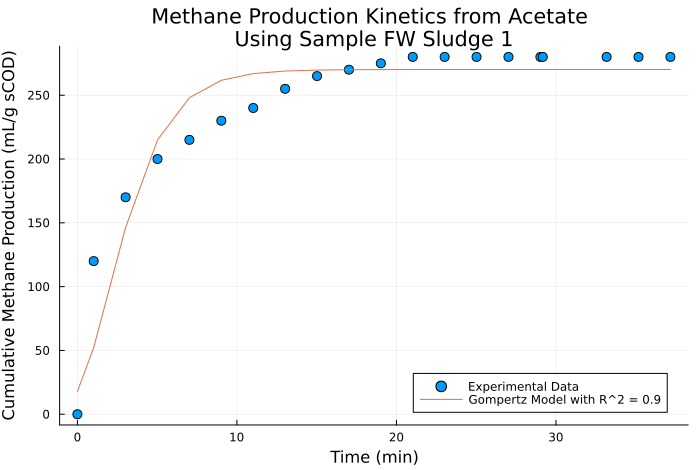
\includegraphics[width=.9\linewidth]{../plots/BMPs/Acetate/methane_kinetics_acet_test_fw_s1.png}
\end{center}

\subsection{Acetate Test 0}
\label{sec:org14c18f5}
Το section αυτό αναφέρεται στη δοκιμή με 100 μL οξικό στο δείγμα (0).

\textbf{acet\textsubscript{test}\textsubscript{0}\textsubscript{s1}}
\begin{minted}[breaklines=true,breakanywhere=true]{julia}

### Data Analysis on Sample 0 ###

<<date_saving_acetate_s1>>

inds = 34:58
exp_meth_vol = [0, 4, 12, 7.5, 4.5, 2.5, 2.5, 4, 0.5, 2, 2, 1, 1, 1, 1, 1, 0.5, 0.5, 0, 0, 0, 0, 0, 0, 0]
meth_vol_acet_0 = cumsum(exp_meth_vol)[end]
exp_name = "acet_test_0_s1"
source = "Acetate"
sample = "Sample 0"
sludge = "Sludge 1"
input_cod = 0.1
p0 = [400.0, 80.0, 1.0]

<<bmp_data_processing>>
<<bmp_curve_fitting_min>>
model_acet_0 = vcat(sample, model_params, r_squared)
<<bmp_data_plotting>>
\end{minted}

\begin{table}[htbp]
\caption{Κινητικά δεδομένα}
\centering
\begin{tabular}{lrrrr}
Timestamp & Seconds & Minutes & Methane\textsubscript{Volume} & Cumulative\textsubscript{Methane}\textsubscript{Volume}\\[0pt]
\hline
29/03\textsubscript{12}:23 & 0.0 & 0.0 & 0.0 & 0.0\\[0pt]
29/03\textsubscript{12}:23 & 13.967 & 0.2328 & 4.0 & 4.0\\[0pt]
29/03\textsubscript{12}:24 & 73.986 & 1.2331 & 12.0 & 16.0\\[0pt]
29/03\textsubscript{12}:25 & 133.981 & 2.233 & 7.5 & 23.5\\[0pt]
29/03\textsubscript{12}:26 & 193.993 & 3.2332 & 4.5 & 28.0\\[0pt]
29/03\textsubscript{12}:27 & 230.339 & 3.839 & 2.5 & 30.5\\[0pt]
29/03\textsubscript{12}:28 & 290.327 & 4.8388 & 2.5 & 33.0\\[0pt]
29/03\textsubscript{12}:29 & 350.322 & 5.8387 & 4.0 & 37.0\\[0pt]
29/03\textsubscript{12}:29 & 363.719 & 6.062 & 0.5 & 37.5\\[0pt]
29/03\textsubscript{12}:30 & 423.727 & 7.0621 & 2.0 & 39.5\\[0pt]
29/03\textsubscript{12}:31 & 483.722 & 8.062 & 2.0 & 41.5\\[0pt]
29/03\textsubscript{12}:32 & 509.669 & 8.4945 & 1.0 & 42.5\\[0pt]
29/03\textsubscript{12}:33 & 569.668 & 9.4945 & 1.0 & 43.5\\[0pt]
29/03\textsubscript{12}:34 & 629.657 & 10.4943 & 1.0 & 44.5\\[0pt]
29/03\textsubscript{12}:35 & 689.661 & 11.4944 & 1.0 & 45.5\\[0pt]
29/03\textsubscript{12}:36 & 749.66 & 12.4943 & 1.0 & 46.5\\[0pt]
29/03\textsubscript{12}:37 & 809.683 & 13.4947 & 0.5 & 47.0\\[0pt]
29/03\textsubscript{12}:38 & 869.926 & 14.4988 & 0.5 & 47.5\\[0pt]
29/03\textsubscript{12}:38 & 910.87 & 15.1812 & 0.0 & 47.5\\[0pt]
29/03\textsubscript{12}:39 & 970.864 & 16.1811 & 0.0 & 47.5\\[0pt]
29/03\textsubscript{12}:40 & 1030.875 & 17.1812 & 0.0 & 47.5\\[0pt]
29/03\textsubscript{12}:41 & 1090.872 & 18.1812 & 0.0 & 47.5\\[0pt]
29/03\textsubscript{12}:42 & 1150.882 & 19.1814 & 0.0 & 47.5\\[0pt]
29/03\textsubscript{12}:43 & 1205.994 & 20.0999 & 0.0 & 47.5\\[0pt]
29/03\textsubscript{12}:44 & 1265.223 & 21.087 & 0.0 & 47.5\\[0pt]
\end{tabular}
\end{table}

\begin{center}
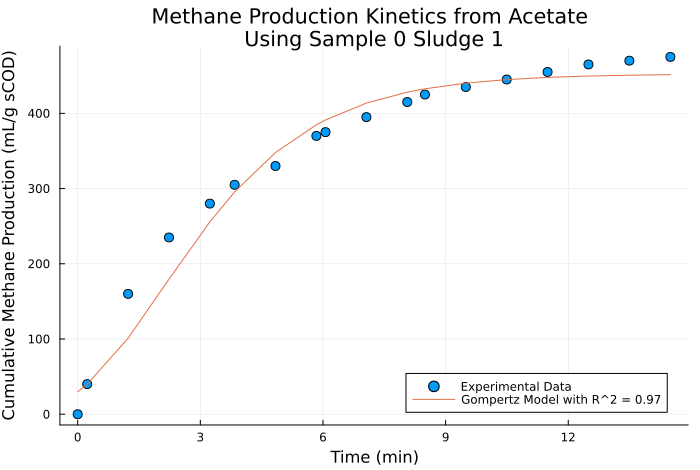
\includegraphics[width=.9\linewidth]{../plots/BMPs/Acetate/methane_kinetics_acet_test_0_s1.png}
\end{center}

\subsection{Acetate Test 1}
\label{sec:orgcbb4c78}
Το section αυτό αναφέρεται στη δοκιμή με 100 μL οξικό στο δείγμα (1). Aξίζει να αναφερθεί πως την πρώτη πειραματική ημέρα (27/03), παρήγαγε αέριο χωρίς να τροφοδοτηθεί με κάποιο υπόστρωμα. Η κινητική αυτής της παραγωγής (η οποία δεν ξέρουμε σε τι ευθύνεται) θα αναλυθεί παρακάτω. Βέβαια, μόλις τροφοδοτήθηκε με οξικό και η παραγωγή του τελείωσε, σταμάτησε και εκείνη η παραγωγή. Βέβαια, είχε την χαμηλότερη παραγωγή βιοαερίου μόλις τροφοδοτήθηκε με οξικό, οπότε ενδέχεται αυτή η μέτρηση να ήταν προβληματική.

\textbf{acet\textsubscript{test}\textsubscript{1}\textsubscript{s1}}
\begin{minted}[breaklines=true,breakanywhere=true]{julia}

### Data Analysis on Sample 1 ###

<<date_saving_acetate_s1>>

inds = 38:58
exp_meth_vol = [0, 6.5, 5, 3, 0.5, 1.5, 1.5, 0.5, 1, 0.5, 0.5, 0.3, 0.2, 0.2, 0.1, 0.05, 0.05, 0.05, 0.05, 0, 0]
meth_vol_acet_1 = cumsum(exp_meth_vol)[end]
exp_name = "acet_test_1_s1"
source = "Acetate"
sample = "Sample 1"
sludge = "Sludge 1"
input_cod = 0.1
p0 = [200.0, 40.0, 1.0]

<<bmp_data_processing>>
<<bmp_curve_fitting_min>>
model_acet_1 = vcat(sample, model_params, r_squared)
<<bmp_data_plotting>>
\end{minted}

\begin{table}[htbp]
\caption{Κινητικά δεδομένα}
\centering
\begin{tabular}{lrrrr}
Timestamp & Seconds & Minutes & Methane\textsubscript{Volume} & Cumulative\textsubscript{Methane}\textsubscript{Volume}\\[0pt]
\hline
29/03\textsubscript{12}:26 & 0.0 & 0.0 & 0.0 & 0.0\\[0pt]
29/03\textsubscript{12}:27 & 36.346 & 0.6058 & 6.5 & 6.5\\[0pt]
29/03\textsubscript{12}:28 & 96.334 & 1.6056 & 5.0 & 11.5\\[0pt]
29/03\textsubscript{12}:29 & 156.329 & 2.6055 & 3.0 & 14.5\\[0pt]
29/03\textsubscript{12}:29 & 169.726 & 2.8288 & 0.5 & 15.0\\[0pt]
29/03\textsubscript{12}:30 & 229.734 & 3.8289 & 1.5 & 16.5\\[0pt]
29/03\textsubscript{12}:31 & 289.729 & 4.8288 & 1.5 & 18.0\\[0pt]
29/03\textsubscript{12}:32 & 315.676 & 5.2613 & 0.5 & 18.5\\[0pt]
29/03\textsubscript{12}:33 & 375.675 & 6.2613 & 1.0 & 19.5\\[0pt]
29/03\textsubscript{12}:34 & 435.664 & 7.2611 & 0.5 & 20.0\\[0pt]
29/03\textsubscript{12}:35 & 495.668 & 8.2611 & 0.5 & 20.5\\[0pt]
29/03\textsubscript{12}:36 & 555.667 & 9.2611 & 0.3 & 20.8\\[0pt]
29/03\textsubscript{12}:37 & 615.69 & 10.2615 & 0.2 & 21.0\\[0pt]
29/03\textsubscript{12}:38 & 675.933 & 11.2656 & 0.2 & 21.2\\[0pt]
29/03\textsubscript{12}:38 & 716.877 & 11.948 & 0.1 & 21.3\\[0pt]
29/03\textsubscript{12}:39 & 776.871 & 12.9479 & 0.05 & 21.35\\[0pt]
29/03\textsubscript{12}:40 & 836.882 & 13.948 & 0.05 & 21.4\\[0pt]
29/03\textsubscript{12}:41 & 896.879 & 14.948 & 0.05 & 21.45\\[0pt]
29/03\textsubscript{12}:42 & 956.889 & 15.9482 & 0.05 & 21.5\\[0pt]
29/03\textsubscript{12}:43 & 1012.001 & 16.8667 & 0.0 & 21.5\\[0pt]
29/03\textsubscript{12}:44 & 1071.23 & 17.8538 & 0.0 & 21.5\\[0pt]
\end{tabular}
\end{table}

\begin{center}
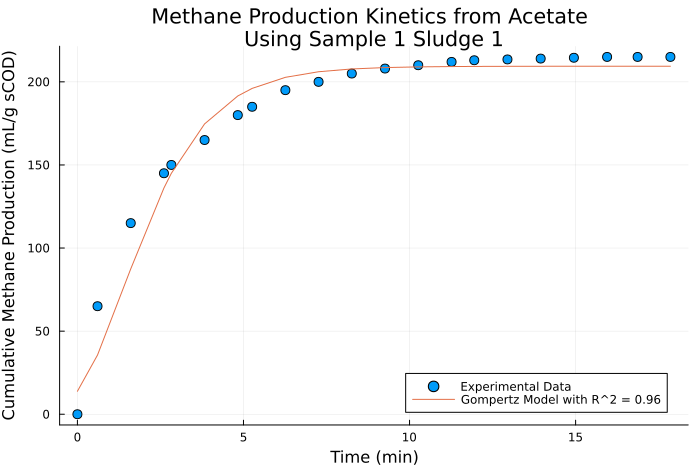
\includegraphics[width=.9\linewidth]{../plots/BMPs/Acetate/methane_kinetics_acet_test_1_s1.png}
\end{center}

\subsection{Acetate Test 2}
\label{sec:orgf22178a}
Το section αυτό αναφέρεται στη δοκιμή με 100 μL οξικό στο δείγμα (2).

\textbf{acet\textsubscript{test}\textsubscript{2}\textsubscript{s1}}
\begin{minted}[breaklines=true,breakanywhere=true]{julia}

### Data Analysis on Sample 2 ###

<<date_saving_acetate_s1>>

inds = 44:58
exp_meth_vol = [0, 4, 7, 5.5, 4.5, 2.5, 2, 1, 1, 1, 0.5, 0.5, 0.45, 0.05, 0]
meth_vol_acet_2 = cumsum(exp_meth_vol)[end]
exp_name = "acet_test_2_s1"
source = "Acetate"
sample = "Sample 2"
sludge = "Sludge 1"
input_cod = 0.1
p0 = [300.0, 60.0, 1.0]

<<bmp_data_processing>>
<<bmp_curve_fitting_min>>
model_acet_2 = vcat(sample, model_params, r_squared)
<<bmp_data_plotting>>
\end{minted}

\begin{table}[htbp]
\caption{Κινητικά Δεδομένα}
\centering
\begin{tabular}{lrrrr}
Timestamp & Seconds & Minutes & Methane\textsubscript{Volume} & Cumulative\textsubscript{Methane}\textsubscript{Volume}\\[0pt]
\hline
29/03\textsubscript{12}:31 & 0.0 & 0.0 & 0.0 & 0.0\\[0pt]
29/03\textsubscript{12}:32 & 25.947 & 0.4324 & 4.0 & 4.0\\[0pt]
29/03\textsubscript{12}:33 & 85.946 & 1.4324 & 7.0 & 11.0\\[0pt]
29/03\textsubscript{12}:34 & 145.935 & 2.4322 & 5.5 & 16.5\\[0pt]
29/03\textsubscript{12}:35 & 205.939 & 3.4323 & 4.5 & 21.0\\[0pt]
29/03\textsubscript{12}:36 & 265.938 & 4.4323 & 2.5 & 23.5\\[0pt]
29/03\textsubscript{12}:37 & 325.961 & 5.4327 & 2.0 & 25.5\\[0pt]
29/03\textsubscript{12}:38 & 386.204 & 6.4367 & 1.0 & 26.5\\[0pt]
29/03\textsubscript{12}:38 & 427.148 & 7.1191 & 1.0 & 27.5\\[0pt]
29/03\textsubscript{12}:39 & 487.142 & 8.119 & 1.0 & 28.5\\[0pt]
29/03\textsubscript{12}:40 & 547.153 & 9.1192 & 0.5 & 29.0\\[0pt]
29/03\textsubscript{12}:41 & 607.15 & 10.1192 & 0.5 & 29.5\\[0pt]
29/03\textsubscript{12}:42 & 667.16 & 11.1193 & 0.45 & 29.95\\[0pt]
29/03\textsubscript{12}:43 & 722.272 & 12.0379 & 0.05 & 30.0\\[0pt]
29/03\textsubscript{12}:44 & 781.501 & 13.025 & 0.0 & 30.0\\[0pt]
\end{tabular}
\end{table}

\begin{center}
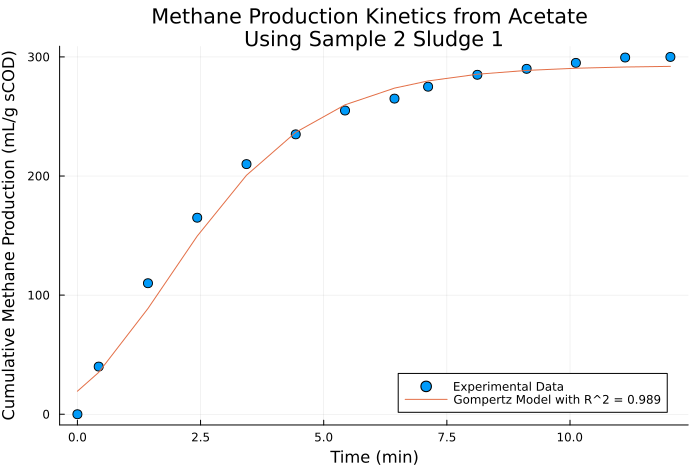
\includegraphics[width=.9\linewidth]{../plots/BMPs/Acetate/methane_kinetics_acet_test_2_s1.png}
\end{center}

\subsection{Acetate Test 4}
\label{sec:org5c5c831}
Το section αυτό αναφέρεται στη δοκιμή με 100 μL οξικό στο δείγμα (4).

\textbf{acet\textsubscript{test}\textsubscript{4}\textsubscript{s1}}
\begin{minted}[breaklines=true,breakanywhere=true]{julia}

### Data Analysis on Sample 4 ###

<<date_saving_acetate_s1>>

inds = 41:58
exp_meth_vol = [0, 4, 10, 9, 4, 5, 5, 4, 3, 3, 0, 0, 0, 0, 0, 0, 0, 0]
meth_vol_acet_4 = cumsum(exp_meth_vol)[end]
exp_name = "acet_test_4_s1"
source = "Acetate"
sample = "Sample 4"
sludge = "Sludge 1"
input_cod = 0.1
p0 = [400.0, 100.0, 1.0]

<<bmp_data_processing>>
<<bmp_curve_fitting_min>>
model_acet_4 = vcat(sample, model_params, r_squared)
<<bmp_data_plotting>>
\end{minted}

\begin{table}[htbp]
\caption{Κινητικά δεδομένα}
\centering
\begin{tabular}{lrrrr}
Timestamp & Seconds & Minutes & Methane\textsubscript{Volume} & Cumulative\textsubscript{Methane}\textsubscript{Volume}\\[0pt]
\hline
29/03\textsubscript{12}:29 & 0.0 & 0.0 & 0 & 0.0\\[0pt]
29/03\textsubscript{12}:29 & 13.397 & 0.2233 & 4 & 4.0\\[0pt]
29/03\textsubscript{12}:30 & 73.405 & 1.2234 & 10 & 14.0\\[0pt]
29/03\textsubscript{12}:31 & 133.4 & 2.2233 & 9 & 23.0\\[0pt]
29/03\textsubscript{12}:32 & 159.347 & 2.6558 & 4 & 27.0\\[0pt]
29/03\textsubscript{12}:33 & 219.346 & 3.6558 & 5 & 32.0\\[0pt]
29/03\textsubscript{12}:34 & 279.335 & 4.6556 & 5 & 37.0\\[0pt]
29/03\textsubscript{12}:35 & 339.339 & 5.6556 & 4 & 41.0\\[0pt]
29/03\textsubscript{12}:36 & 399.338 & 6.6556 & 3 & 44.0\\[0pt]
29/03\textsubscript{12}:37 & 459.361 & 7.656 & 3 & 47.0\\[0pt]
29/03\textsubscript{12}:38 & 519.604 & 8.6601 & 0 & 47.0\\[0pt]
29/03\textsubscript{12}:38 & 560.548 & 9.3425 & 0 & 47.0\\[0pt]
29/03\textsubscript{12}:39 & 620.542 & 10.3424 & 0 & 47.0\\[0pt]
29/03\textsubscript{12}:40 & 680.553 & 11.3425 & 0 & 47.0\\[0pt]
29/03\textsubscript{12}:41 & 740.55 & 12.3425 & 0 & 47.0\\[0pt]
29/03\textsubscript{12}:42 & 800.56 & 13.3427 & 0 & 47.0\\[0pt]
29/03\textsubscript{12}:43 & 855.672 & 14.2612 & 0 & 47.0\\[0pt]
29/03\textsubscript{12}:44 & 914.901 & 15.2484 & 0 & 47.0\\[0pt]
\end{tabular}
\end{table}

\begin{center}
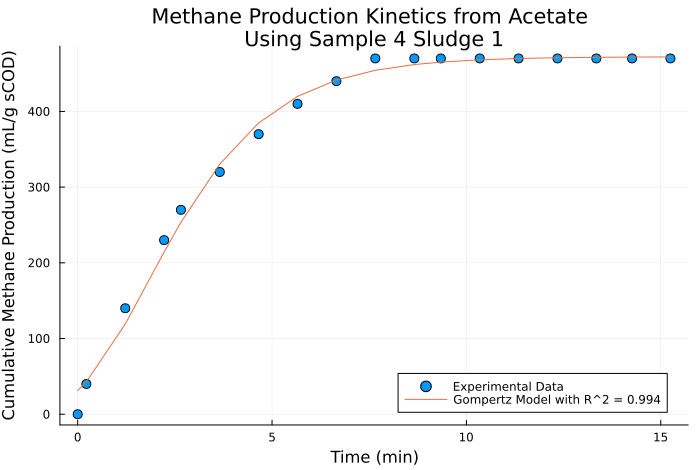
\includegraphics[width=.9\linewidth]{../plots/BMPs/Acetate/methane_kinetics_acet_test_4_s1.png}
\end{center}

\subsection{Παραγωγή μεθανίου χωρίς feed από το δείγμα Ac}
\label{sec:orgaab3c29}
Όπως προαναφέρθηκε, το δείγμα Ac παρήγαγε μεθάνιο χωρίς να τροφοδοτηθεί με κάτι για κάποιον ανεξήγητο λόγο. Καθώς έχουμε πειραματικά δεδομένα για αυτή την κατανάλωση (και μάλιστα 2 data sets), θα γίνει και μία ανάλυση για αυτό.

\textbf{no\textsubscript{feed}\textsubscript{ac}\textsubscript{1}}
\begin{minted}[breaklines=true,breakanywhere=true]{julia}

### No Feed Data Analysis ###

<<date_saving_acetate_s1>>

inds = 1:17
exp_meth_vol = [0, 9, 3, 2, 3, 3, 3, 2.5, 2.5, 2.5, 1.5, 3, 1, 1, 1.5, 0.5, 0.1]
exp_name = "no_feed_ac_1"
source = "No_Feed"
sample = "Sample Ac"
sludge = "Sludge 1"
kinetics = false

<<bmp_data_processing>>
<<bmp_data_plotting>>
\end{minted}

\textbf{no\textsubscript{feed}\textsubscript{ac}\textsubscript{2}}
\begin{minted}[breaklines=true,breakanywhere=true]{julia}

<<date_saving_acetate_s1>>

inds = 18:33
exp_meth_vol = [0, 3, 2, 2, 2, 3, 2, 2, 3, 2, 2.5, 2.5, 2, 2.5, 2.5, 2]
exp_name = "no_feed_ac_2"
source = "No_Feed"
sample = "Sample Ac"
sludge = "Sludge 1"
kinetics = false

<<bmp_data_processing>>
<<bmp_data_plotting>>
\end{minted}

\subsection{Update all helper}
\label{sec:org21a3ada}
Σε αυτό το section θα υπάρχει ένα helper code block που θα κάνει evaluate όλα τα παραπάνω. Έτσι, αν αλλάξει κάτι το οποίο επηρεάζει περισσότερα από ένα code blocks, θα μπορούν να γίνουν updated ταυτόχρονα πιο εύκολα. Επίσης, μία επιπλέον χρησιμότητα του code block αυτού είναι ότι αποθηκεύει ένα CSV που συγκεντρώνει όλα τα δεδομένα των κινητικών παραμέτρων από την προσαρμογή που έγινε παραπάνω, το οποίο είναι χρήσιμο για συγκρίσεις, παρόλο που τα συγκεκριμένα πειράματα δεν είναι τόσο σημαντικό να συγκριθούν.

\textbf{update\textsubscript{acetate}\textsubscript{tests}\textsubscript{s1}}
\begin{minted}[breaklines=true,breakanywhere=true]{julia}

<<acet_test_0_s1>>
<<acet_test_1_s1>>
<<acet_test_2_s1>>
<<acet_test_4_s1>>
<<acet_test_FW_s1>>
<<no_feed_ac_1>>
<<no_feed_ac_2>>

model_fit_table = Tables.table(vcat(reshape(model_acet_0, 1, 5), reshape(model_acet_1, 1, 5), reshape(model_acet_2, 1, 5), reshape(model_acet_4, 1, 5), reshape(model_acet_fw, 1, 5)), header = [:Sample_Name, :Methane_Production_Potential, :Methane_Production_Rate, :Lag_Time, :R_squared])
CSV.write(datadir("exp_pro", "methane_from_acetate_kinetics_s1.csv"), model_fit_table)
DataFrame(model_fit_table)

\end{minted}

\begin{table}[htbp]
\caption{Kinetic Models}
\centering
\begin{tabular}{lrrrr}
Sample\textsubscript{Name} & Production\textsubscript{Potential} & Production\textsubscript{Rate} & Lag\textsubscript{Time} & R\textsubscript{squared}\\[0pt]
\hline
Sample 0 & 466.328 & 76.639 & 0.0 & 0.971\\[0pt]
Sample 1 & 209.405 & 54.484 & 0.0 & 0.960\\[0pt]
Sample 2 & 293.893 & 62.335 & 0.0 & 0.990\\[0pt]
Sample 4 & 472.276 & 96.498 & 0.0 & 0.994\\[0pt]
Sample FW & 270.141 & 49.008 & 0.0 & 0.900\\[0pt]
\end{tabular}
\end{table}

\subsection{Γενικά σχόλια για αυτόν τον κύκλο πειραμάτων}
\label{sec:org7cfc4b6}
Ο πρώτος αυτός κύκλος πειραμάτων ήταν για την δοκιμή προσθήκης οξικού οξέος, του ιδανικού υποστρώματος της μεθανογένεσης, για να δούμε πως θα αντιδράσει σε αυτό το σύστημα. Δεν έχει τόσο συγκριτικό χαρακτήρα μεταξύ των πειραμάτων (παρόλο που ένα σχόλιο που μπορεί να γίνει είναι πως τα πειράματα τα οποία ήταν ίδια πρακτικά στην αρχή, είχαν αρκετά διαφορετική απόκριση στην προσθήκη οξικού), αλλά τον χαρακτήρα της βέλτιστης δυνατής μεθανογένεσης από κάποιο υπόστρωμα. Από την μελέτη αυτή, προέκυψαν αρκετά συμπεράσματα.

Ένα ενδιαφέρον σχόλιο είναι πως το σύστημα ανταποκρίνεται στην προσθήκη του οξικού πολύ γρήγορα (μετά από μερικά δευτερόλεπτα κιόλας βλέπουμε παραγωγή μεθανίου) και στο μοντέλο αυτό μεταφράζεται ως μηδενικό lag-phase.

Το δείγμα 4 είχε αναπάντεχα υψηλό ρυθμό παραγωγής μεθανίου, το οποίο φάνηκε από το γεγονός ότι παράχθηκε την μέγιστη ποσότητα οξικού που περιμέναμε σε περίπου 7 λεπτά ενώ τα υπόλοιπα χρειάστηκαν τουλάχιστον 15 λεπτά. Αυτό φάνηκε και στο μοντέλο, όπου το δείγμα αυτό είχε πολύ υψηλό ειδικό ρυθμό παραγωγής μεθανίου. Το δείγμα Ac ήταν αυτό που παρήγαγε αέριο χωρίς κάποιο υπόστρωμα. Μόλις προστέθηκε οξικό, αντέδρασε σε αυτό και ο ρυθμός του αυξήθηκε, αλλά επιβράδυνε πολύ γρήγορα, με αποτέλεσμα να έχει πολύ αργό ρυθμό παραγωγής μεθανίο και το χαμηλότερο δυναμικό παραγωγής μεθανίου. Μπορεί η αλλαγή αυτή να ευθύνεται σε αυτήν την απόκριση. Τα δείγματα 0 και 4 είχαν πολύ μεγαλύτερη παραγωγικότητα από τα άλλα 3, χωρίς να υπάρχει κάποια εύκολη εξήγηση για αυτό.

\pagebreak

\section{FW Hydrolysate S1\textsubscript{R1} Processing}
\label{sec:org900e8d4}
Στο section αυτό θα αναλυθούν τα αποτελεσματα του πρώτου πειράματος που χρησιμοποιήσε FW hydrolysate ως υπόστρωμα (συμβολίζεται ως S1\textsubscript{R1} επειδή είναι το πρώτο run με την πρώτη λάσπη). Σκοπός είναι να γίνει μία σύγκριση αυτού με το οξικό για κάθε δοχείο για να προκύψουν αποτελέσματα για το κάθε πείραμα. Οι 5 δοκιμές που έγιναν ήταν στα δείγματα 0, 1, 2 και 4 (τα οποία πλέον έχουν νόημα επειδή εκφράζουν την ποσότητα mix που προστέθηκε κατά την υδρόλυση) αλλά επίσης έγινε και ένα πείραμα για να μετρηθεί η απόδοση σε μεθάνιο του δείγματος μόνο με FW (ενδέχεται να υπήρξε διαρροή στο δείγμα αυτό καθώς η παραγωγή ήταν απειροελάχιστη).

\subsection{Sample 0}
\label{sec:orgbfa858d}
Το δείγμα αυτό είναι labelled ως δείγμα 0 καθώς είναι το δείγμα το οποίο τροφοδοτήθηκε με treated FW, όμως χωρίς προσθήκη του μιξ ενζύμων και μικροοργανισμών. Όπως έχουμε δεί, όλες οι αντιδράσεις που γίνονται κατά την υδρόλυση και ζύμωση μπορούν να γίνουν και χωρίς το μιξ. Όμως, γινόντουσαν πιο αποτελεσματικά με την προσθήκη αυτού. Οπότε, ελπίζουμε πως το δείγμα αυτό θα έχει χειρότερα αποτελέσματα από τα άλλα, το οποίο θα μας οδηγήσει στην υπόθεση ότι το μιξ βελτιώνει όχι μόνο τα κριτήρια υδρόλυσης και οξεογένεσης αλλά και αυτό της μεθανογένεσης.

\textbf{hydrolysate\textsubscript{0}\textsubscript{s1}\textsubscript{r1}}
\begin{minted}[breaklines=true,breakanywhere=true]{julia}

### Data Analysis on Hydrolysate with 0 ml ###

<<date_saving_fw_s1_r1>>

inds = 1:40
exp_meth_vol = [0, 1.0, 0.2, 0.02, 0.02, 0.01, 0.2, 0.2, 0.5, 0.2, 0.5, 1.5, 0.05, 0.05, 0.05, 0.05, 0.05, 0.05, 0.1, 0.1, 0.1, 0.1, 0.1, 0.1, 0.1, 0.1, 0.1, 0.1, 0.1, 0.1, 0.1, 0.05, 0.05, 0.05, 0, 0, 0, 0, 0, 0]
meth_vol_hydro_0 = cumsum(exp_meth_vol)[end]

exp_name = "hydrolysate_0_s1_r1"
source = "Hydrolyzed FW"
sample = "Sample 0"
sludge = "Sludge 1"
run_num = "Run 1"
input_cod = 0.1

<<bmp_data_processing>>

# The same model is fit either with min or hour
p0 = [50.0, 0.4, 1.0]
<<bmp_curve_fitting_min>>
model_hydro_0_min = vcat(sample, model_params, r_squared)
<<bmp_data_plotting>>

p0 = [40.0, 1.0, 1.0]
<<bmp_curve_fitting_hour>>
model_hydro_0_hour = vcat(sample, model_params, r_squared)
<<bmp_data_plotting>>
\end{minted}

\begin{verbatim}
sys:1: UserWarning: No data for colormapping provided via 'c'. Parameters 'vmin', 'vmax' will be ignored
sys:1: UserWarning: No data for colormapping provided via 'c'. Parameters 'vmin', 'vmax' will be ignored
sys:1: UserWarning: No data for colormapping provided via 'c'. Parameters 'vmin', 'vmax' will be ignored
sys:1: UserWarning: No data for colormapping provided via 'c'. Parameters 'vmin', 'vmax' will be ignored
sys:1: UserWarning: No data for colormapping provided via 'c'. Parameters 'vmin', 'vmax' will be ignored
sys:1: UserWarning: No data for colormapping provided via 'c'. Parameters 'vmin', 'vmax' will be ignored
"/home/vidianos/Documents/9o_εξάμηνο/Masters_Thesis/plots/BMPs/Hydrolyzed FW/methane_kinetics_hydrolysate_0_hour.png"
\end{verbatim}

\subsubsection{Results}
\label{sec:org31b66cd}
Παρακάτω φαίνονται τα αποτελέσματα του σχετικού πειράματος.

Παρήγαγε 6.1 ml μεθανίου, το οποίο είναι το \(12.8 \%\) του πειράματος με οξικό. Σχετικά με την προσαρμογή των δεδομένων του σε ένα μοντέλο Gompertz, υπάρχουν 2 πιθανά μοντέλα που ταιριάζουν στο πείραμα. Στο πρώτο, ο ειδικός ρυθμός ανάπτυξης είναι μεγάλος, το οποίο κάνει fit τέλεια στις μετρήσεις της πρώτης ώρας όπου η παραγωγή είναι γρήγορη. Όμως, προβλέπει την στάσιμη φάση λίγες ώρες μετά, το οποίο δεν ισχύει καθώς την 2η μέρα υπάρχει μία καλή παραγωγικότητα μεθανίου. Παρόλα αυτά, έχει καλό R\textsuperscript{2}. Αυτό το μοντέλο είναι πιο εύκολο να προβλεφθεί με x άξονα σε λεπτά, όπου δεν χρειάζεται πάρα πολύ υψηλή αρχική συνθήκη. Ο προβλεπόμενος ειδικός ρυθμός ανάπτυξης θα είναι \(0.384 \frac{ml}{g ~ sCOD \min } \text{ ή } 23.03 \frac{ml}{g ~ sCOD hour}\).

Όμως, υπάρχει και ένα δεύτερο μοντέλο με καλή προσαρμογή (μάλιστα είναι ελαφρώς καλύτερη). Αν ο ειδικός ρυθμός ανάπτυξης είναι χαμηλός, υπάρχει μοντέλο που προσαρμόζεται σχεδόν τέλεια στην 2η και 3η μέρα. Συγκεκριμένα, με ειδικό ρυθμό \(1.636 \frac{ml}{g ~ sCOD ~ hour}\) πετυχαίνεται μία πολύ καλή προσαρμογή. Όμως, αυτό είναι αρκετά λάθος για την πρώτη μέρα.

Ένα πιθανό συμπέρασμα μπορεί να είναι πως κάτι συμβαίνει στον αντιδραστήρα το οποίο επιβραδύνει σημαντικά τον μέγιστο ειδικό ρυθμό ανάπτυξης, ο οποίος μπαίνει στο μοντέλο.

\begin{center}
\begin{tabular}{lrrrr}
Timestamp & Minutes & Hours & Methane\textsubscript{Volume} & Cumulative\textsubscript{Methane}\textsubscript{Volume}\\[0pt]
\hline
01/04\textsubscript{11}:05 & 0.0 & 0.0 & 0.0 & 0.0\\[0pt]
01/04\textsubscript{11}:09 & 3.7328 & 0.0622 & 1.0 & 1.0\\[0pt]
01/04\textsubscript{11}:11 & 5.733 & 0.0956 & 0.2 & 1.2\\[0pt]
01/04\textsubscript{11}:12 & 6.7332 & 0.1122 & 0.02 & 1.22\\[0pt]
01/04\textsubscript{11}:13 & 7.5618 & 0.126 & 0.02 & 1.24\\[0pt]
01/04\textsubscript{11}:14 & 8.5617 & 0.1427 & 0.01 & 1.25\\[0pt]
01/04\textsubscript{11}:15 & 9.5618 & 0.1594 & 0.2 & 1.45\\[0pt]
01/04\textsubscript{11}:21 & 16.0005 & 0.2667 & 0.2 & 1.65\\[0pt]
01/04\textsubscript{11}:52 & 46.3266 & 0.7721 & 0.5 & 2.15\\[0pt]
01/04\textsubscript{12}:22 & 76.3266 & 1.2721 & 0.2 & 2.35\\[0pt]
01/04\textsubscript{16}:52 & 346.3272 & 5.7721 & 0.5 & 2.85\\[0pt]
02/04\textsubscript{10}:54 & 1428.1379 & 23.8023 & 1.5 & 4.35\\[0pt]
02/04\textsubscript{12}:54 & 1548.1453 & 25.8024 & 0.05 & 4.4\\[0pt]
02/04\textsubscript{13}:24 & 1578.1452 & 26.3024 & 0.05 & 4.45\\[0pt]
02/04\textsubscript{13}:54 & 1608.1455 & 26.8024 & 0.05 & 4.5\\[0pt]
02/04\textsubscript{14}:24 & 1638.1455 & 27.3024 & 0.05 & 4.55\\[0pt]
02/04\textsubscript{14}:54 & 1668.1454 & 27.8024 & 0.05 & 4.6\\[0pt]
02/04\textsubscript{15}:24 & 1698.1453 & 28.3024 & 0.05 & 4.65\\[0pt]
02/04\textsubscript{15}:54 & 1728.1453 & 28.8024 & 0.1 & 4.75\\[0pt]
02/04\textsubscript{16}:24 & 1758.1455 & 29.3024 & 0.1 & 4.85\\[0pt]
02/04\textsubscript{16}:54 & 1788.1455 & 29.8024 & 0.1 & 4.95\\[0pt]
02/04\textsubscript{17}:24 & 1818.1452 & 30.3024 & 0.1 & 5.05\\[0pt]
02/04\textsubscript{17}:54 & 1848.152 & 30.8025 & 0.1 & 5.15\\[0pt]
02/04\textsubscript{19}:54 & 1968.1526 & 32.8025 & 0.1 & 5.25\\[0pt]
02/04\textsubscript{21}:54 & 2088.1542 & 34.8026 & 0.1 & 5.35\\[0pt]
02/04\textsubscript{23}:54 & 2208.1584 & 36.8026 & 0.1 & 5.45\\[0pt]
03/04\textsubscript{01}:54 & 2328.1584 & 38.8026 & 0.1 & 5.55\\[0pt]
03/04\textsubscript{03}:54 & 2448.1582 & 40.8026 & 0.1 & 5.65\\[0pt]
03/04\textsubscript{05}:54 & 2568.1632 & 42.8027 & 0.1 & 5.75\\[0pt]
03/04\textsubscript{07}:54 & 2688.1651 & 44.8028 & 0.1 & 5.85\\[0pt]
03/04\textsubscript{09}:54 & 2808.1652 & 46.8028 & 0.1 & 5.95\\[0pt]
03/04\textsubscript{12}:54 & 2988.1741 & 49.8029 & 0.05 & 6.0\\[0pt]
03/04\textsubscript{13}:54 & 3048.1739 & 50.8029 & 0.05 & 6.05\\[0pt]
03/04\textsubscript{14}:24 & 3078.1749 & 51.3029 & 0.05 & 6.1\\[0pt]
03/04\textsubscript{14}:54 & 3108.9336 & 51.8156 & 0.0 & 6.1\\[0pt]
03/04\textsubscript{15}:26 & 3140.9794 & 52.3497 & 0.0 & 6.1\\[0pt]
03/04\textsubscript{16}:29 & 3203.2503 & 53.3875 & 0.0 & 6.1\\[0pt]
03/04\textsubscript{17}:29 & 3263.2548 & 54.3876 & 0.0 & 6.1\\[0pt]
03/04\textsubscript{18}:29 & 3323.2547 & 55.3876 & 0.0 & 6.1\\[0pt]
03/04\textsubscript{20}:29 & 3443.2548 & 57.3876 & 0.0 & 6.1\\[0pt]
\end{tabular}
\end{center}

\begin{center}
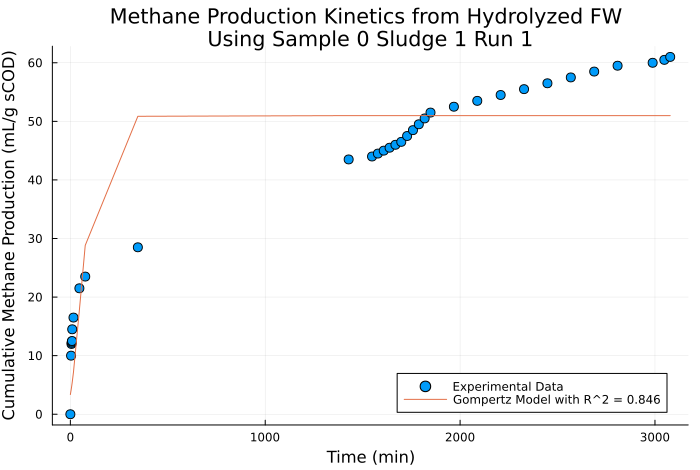
\includegraphics[width=.9\linewidth]{../plots/BMPs/Hydrolyzed FW/methane_kinetics_hydrolysate_0_s1_r1_min.png}
\end{center}

\begin{center}
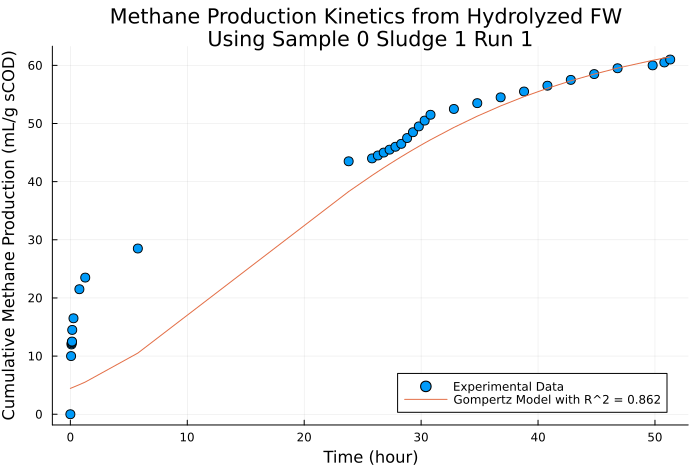
\includegraphics[width=.9\linewidth]{../plots/BMPs/Hydrolyzed FW/methane_kinetics_hydrolysate_0_s1_r1_hour.png}
\end{center}

\subsection{Sample 1}
\label{sec:org1a6b6a6}
Το δείγμα αυτό τροφοδοτήθηκε με το υδρόλυμα το οποίο είχε προσθήκη 1 ml mix. Στο αρχικό κινητικό πείραμα, το δείγμα αυτό είχε αρκετά παρόμοια συμπεριφορά με το 0 και χειρότερη αυτής του 1. Από την μέτρηση του COD του, είχε αναπάντεχα υψηλό sCOD. Αυτό σημαίνει είτε πως έγινε κάποιο λάθος στην ανάλυση ή ότι απλώς έγινε πολύ καλύτερη υδρόλυση από ότι περιμέναμε στο πείραμα αυτό. Με βάση το sCOD του, αναμένεται να έχει καλά αποτελέσματα. Με βάση την HPLC του αρχικού πειράματος, θα περιμέναμε να είναι λίγο καλύτερο από το 0.

\textbf{hydrolysate\textsubscript{1}\textsubscript{s1}\textsubscript{r1}}
\begin{minted}[breaklines=true,breakanywhere=true]{julia}

### Data Analysis on Hydrolysate with 1 ml ###

<<date_saving_fw_s1_r1>>

inds = 2:40
exp_meth_vol = [0, 2.0, 0.5, 0.5, 0.5, 0.5, 0.5, 0, 0.2, 0.5, 2.0, 0.3, 0.3, 0.3, 0.1, 0.6, 0.6, 0.5, 0.5, 0.5, 0.4, 0.6, 0.1, 0.05, 0.05, 0.05, 0.05, 0.05, 0.05, 0.05, 0.3, 0.2, 0.2, 0, 0, 0, 0, 0, 0]
meth_vol_hydro_1 = cumsum(exp_meth_vol)[end]
exp_name = "hydrolysate_1_s1_r1"
source = "Hydrolyzed FW"
sample = "Sample 1"
sludge = "Sludge 1"
run_num = "Run 1"
input_cod = 0.1

p0 = [130.0, 10.0, 1.0]
<<bmp_data_processing>>
<<bmp_curve_fitting_min>>
model_hydro_1_min = vcat(sample, model_params, r_squared)
<<bmp_data_plotting>>

p0 = [200.0, 5.0, 1.0]
<<bmp_curve_fitting_hour>>
model_hydro_1_hour = vcat(sample, model_params, r_squared)
<<bmp_data_plotting>>
\end{minted}

\begin{verbatim}
sys:1: UserWarning: No data for colormapping provided via 'c'. Parameters 'vmin', 'vmax' will be ignored
sys:1: UserWarning: No data for colormapping provided via 'c'. Parameters 'vmin', 'vmax' will be ignored
sys:1: UserWarning: No data for colormapping provided via 'c'. Parameters 'vmin', 'vmax' will be ignored
sys:1: UserWarning: No data for colormapping provided via 'c'. Parameters 'vmin', 'vmax' will be ignored
sys:1: UserWarning: No data for colormapping provided via 'c'. Parameters 'vmin', 'vmax' will be ignored
sys:1: UserWarning: No data for colormapping provided via 'c'. Parameters 'vmin', 'vmax' will be ignored
"/home/vidianos/Documents/9o_εξάμηνο/Masters_Thesis/plots/BMPs/Hydrolyzed FW/methane_kinetics_hydrolysate_1_hour.png"
\end{verbatim}

\subsubsection{Results}
\label{sec:orge13dc05}
Το πείραμα αυτό παρήγαγε 13.05 ml μεθάνιο, το οποίο είναι το \(60.7 \%\) του πειράματος με οξικό καθώς εκείνο το πείραμα είχε μία σχετικά χαμηλή παραγωγικότητα για οξικό. Υπάρχει η σκέψη ότι μπορεί λόγω της διεργασίας που συνέβαινε αρχικά στο δείγμα αυτό (παραγωγή μεθανίου χωρίς τροφή) να επηρεάστηκε η παραγωγικότητα του και αυτό το ποσοστό να μην είναι τόσο έμπιστο.

Από άποψη προσαρμογής, το πείραμα αυτό έχει το πρόβλημα πως μεταξύ της 2ης και 3ης μέρας όχι μόνο επιβραδύνθηκε αρκετά το πείραμα (όπως στο 0 ml) αλλά σχεδόν σταμάτησε. Όμως, το πρωί της τρίτης μέρας, λίγο πριν σταματήσουμε το πείραμα, η παραγωγή αυξήθηκε σχετικά σημαντικά. Οπότε, η προσαρμογή του είναι λίγο πιο δύσκολη. Υπάρχει πάλι το φαινόμενο των 2 ρυθμών (ενός γρήγορου για τα δείγματα της 1ης μέρας και ενός αργού για μετά), όμως, ο γρήγορος είναι σημαντικά χειρότερος εδώ (R\textsuperscript{2} 0.689 αντί για 0.815), προβλέπει με λιγότερη ακρίβεια ακόμη και την πρώτη μέρα και η στάσιμη φάση του είναι πολύ χαμηλά. Ο αργός ρυθμός είναι και αυτός σχετικά λάθος επειδή δεν μπορεί να προβλέψει την δημιουργία στάσιμης φάσης και μετά επανεκίννησης της χώνευσης (κάτι που δεν νομίζω να προβλέπεται από οποιοδήποτε μοντέλο). Οπότε, κάνει underestimate το σημείο που ακόμη παράγει και overestimate όταν έχει αρχίσει η στάσιμη φάση. Βέβαια, για τόσα πειραματικά σημεία (τα οποία έχουν και κάποια προβλήματα που δεν μπορούν να εξηγηθούν εύκολα), η προσαρμογή με R\textsuperscript{2} = 0.815 είναι σχετικά καλή.

Το μοντέλο με τον γρήγορο ρυθμό έχει ειδικό ρυθμό ανάπτυξης \(0.841 \frac{ml}{g ~ sCOD min } \text{ ή } 50.43 \frac{ml}{g ~ sCOD hour}\) ενώ το αργό έχει ρυθμό \(3.175 \frac{ml}{g ~ sCOD hour}\).

\begin{center}
\begin{tabular}{lrrrr}
Timestamp & Minutes & Hours & Methane\textsubscript{Volume} & Cumulative\textsubscript{Methane}\textsubscript{Volume}\\[0pt]
\hline
01/04\textsubscript{11}:09 & 0.0 & 0.0 & 0.0 & 0.0\\[0pt]
01/04\textsubscript{11}:11 & 2.0003 & 0.0333 & 2.0 & 2.0\\[0pt]
01/04\textsubscript{11}:12 & 3.0004 & 0.05 & 0.5 & 2.5\\[0pt]
01/04\textsubscript{11}:13 & 3.829 & 0.0638 & 0.5 & 3.0\\[0pt]
01/04\textsubscript{11}:14 & 4.8289 & 0.0805 & 0.5 & 3.5\\[0pt]
01/04\textsubscript{11}:15 & 5.8291 & 0.0972 & 0.5 & 4.0\\[0pt]
01/04\textsubscript{11}:21 & 12.2677 & 0.2045 & 0.5 & 4.5\\[0pt]
01/04\textsubscript{11}:52 & 42.5938 & 0.7099 & 0.0 & 4.5\\[0pt]
01/04\textsubscript{12}:22 & 72.5938 & 1.2099 & 0.2 & 4.7\\[0pt]
01/04\textsubscript{16}:52 & 342.5944 & 5.7099 & 0.5 & 5.2\\[0pt]
02/04\textsubscript{10}:54 & 1424.4052 & 23.7401 & 2.0 & 7.2\\[0pt]
02/04\textsubscript{12}:54 & 1544.4126 & 25.7402 & 0.3 & 7.5\\[0pt]
02/04\textsubscript{13}:24 & 1574.4125 & 26.2402 & 0.3 & 7.8\\[0pt]
02/04\textsubscript{13}:54 & 1604.4127 & 26.7402 & 0.3 & 8.1\\[0pt]
02/04\textsubscript{14}:24 & 1634.4127 & 27.2402 & 0.1 & 8.2\\[0pt]
02/04\textsubscript{14}:54 & 1664.4126 & 27.7402 & 0.6 & 8.8\\[0pt]
02/04\textsubscript{15}:24 & 1694.4125 & 28.2402 & 0.6 & 9.4\\[0pt]
02/04\textsubscript{15}:54 & 1724.4125 & 28.7402 & 0.5 & 9.9\\[0pt]
02/04\textsubscript{16}:24 & 1754.4128 & 29.2402 & 0.5 & 10.4\\[0pt]
02/04\textsubscript{16}:54 & 1784.4128 & 29.7402 & 0.5 & 10.9\\[0pt]
02/04\textsubscript{17}:24 & 1814.4125 & 30.2402 & 0.4 & 11.3\\[0pt]
02/04\textsubscript{17}:54 & 1844.4193 & 30.7403 & 0.6 & 11.9\\[0pt]
02/04\textsubscript{19}:54 & 1964.4198 & 32.7403 & 0.1 & 12.0\\[0pt]
02/04\textsubscript{21}:54 & 2084.4214 & 34.7404 & 0.05 & 12.05\\[0pt]
02/04\textsubscript{23}:54 & 2204.4256 & 36.7404 & 0.05 & 12.1\\[0pt]
03/04\textsubscript{01}:54 & 2324.4257 & 38.7404 & 0.05 & 12.15\\[0pt]
03/04\textsubscript{03}:54 & 2444.4255 & 40.7404 & 0.05 & 12.2\\[0pt]
03/04\textsubscript{05}:54 & 2564.4305 & 42.7405 & 0.05 & 12.25\\[0pt]
03/04\textsubscript{07}:54 & 2684.4324 & 44.7405 & 0.05 & 12.3\\[0pt]
03/04\textsubscript{09}:54 & 2804.4325 & 46.7405 & 0.05 & 12.35\\[0pt]
03/04\textsubscript{12}:54 & 2984.4414 & 49.7407 & 0.3 & 12.65\\[0pt]
03/04\textsubscript{13}:54 & 3044.4412 & 50.7407 & 0.2 & 12.85\\[0pt]
03/04\textsubscript{14}:24 & 3074.4422 & 51.2407 & 0.2 & 13.05\\[0pt]
03/04\textsubscript{14}:54 & 3105.2008 & 51.7533 & 0.0 & 13.05\\[0pt]
03/04\textsubscript{15}:26 & 3137.2466 & 52.2874 & 0.0 & 13.05\\[0pt]
03/04\textsubscript{16}:29 & 3199.5175 & 53.3253 & 0.0 & 13.05\\[0pt]
03/04\textsubscript{17}:29 & 3259.522 & 54.3254 & 0.0 & 13.05\\[0pt]
03/04\textsubscript{18}:29 & 3319.522 & 55.3254 & 0.0 & 13.05\\[0pt]
03/04\textsubscript{20}:29 & 3439.522 & 57.3254 & 0.0 & 13.05\\[0pt]
\end{tabular}
\end{center}

\begin{center}
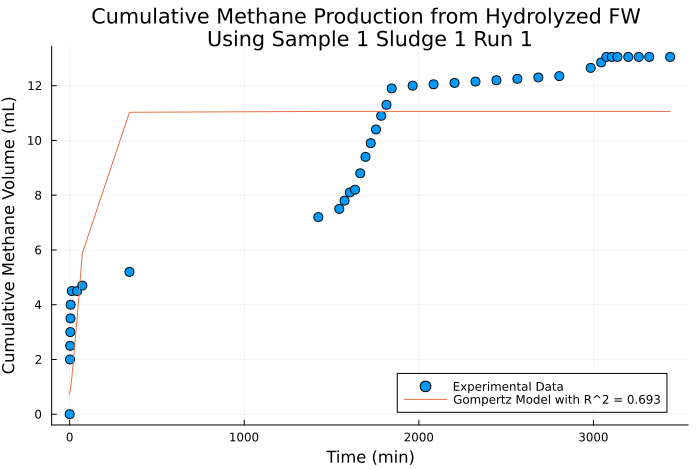
\includegraphics[width=.9\linewidth]{../plots/BMPs/Hydrolyzed FW/methane_kinetics_hydrolysate_1_s1_r1_min.png}
\end{center}

\begin{center}
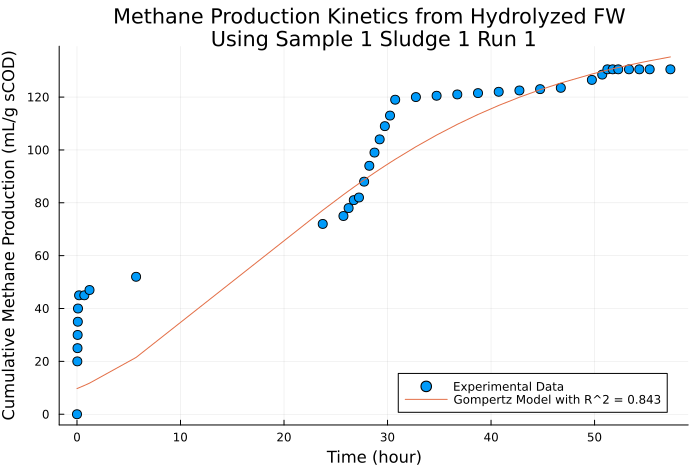
\includegraphics[width=.9\linewidth]{../plots/BMPs/Hydrolyzed FW/methane_kinetics_hydrolysate_1_s1_r1_hour.png}
\end{center}

\subsection{Sample 2}
\label{sec:org82e2b27}
Το δείγμα το οποίο στην υδρόλυση είχε 2 ml από το μιξ. Με βάση το αρχικό πείραμα υδρόλυσης, αυτό και το 4 ml είχαν το καλύτερο performance και ελάχιστη διαφορά μεταξύ τους (κατά βάση στην συγκέντρωση γαλακτικού οξέος) οπότε θα αναμέναμε εδώ να παρατηρηθεί η καλύτερη μεθανογένεση.

\textbf{hydrolysate\textsubscript{2}\textsubscript{s1}\textsubscript{r1}}
\begin{minted}[breaklines=true,breakanywhere=true]{julia}

### Data Analysis on Hydrolysate with 2 ml ###

<<date_saving_fw_s1_r1>>

inds = 7:40
exp_meth_vol = [0, 6, 0.5, 0.1, 0.5, 1.5, 0.2, 0.1, 0.1, 0.1, 0.1, 0.1, 0.1, 0.1, 0.1, 0.1, 0.1, 0.1, 0.1, 0.1, 0.1, 0.1, 0.1, 0.1, 0.1, 0.1, 0.2, 0.2, 0, 0, 0, 0, 0, 0]
meth_vol_hydro_2 = cumsum(exp_meth_vol)[end]
exp_name = "hydrolysate_2_s1_r1"
source = "Hydrolyzed FW"
sample = "Sample 2"
sludge = "Sludge 1"
run_num = "Run 1"
input_cod = 0.1

<<bmp_data_processing>>

p0 = [100.0, 15.0, 1.0]
<<bmp_curve_fitting_min>>
model_hydro_2_min = vcat(sample, model_params, r_squared)
<<bmp_data_plotting>>

p0 = [100.0, 1.0, 0.03]
<<bmp_curve_fitting_hour>>
model_hydro_2_hour = vcat(sample, model_params, r_squared)
<<bmp_data_plotting>>
\end{minted}

\begin{verbatim}
"/home/vidianos/Documents/9o_εξάμηνο/Masters_Thesis/plots/BMPs/Hydrolyzed FW/methane_kinetics_hydrolysate_2_hour.png"
\end{verbatim}

\subsubsection{Results}
\label{sec:org39a0e3d}
Το παραγώμενο μεθάνιο είναι 11.1 ml, δηλαδή \(37 \%\) του προβλεπόμενου μεθανίου με βάση το οξικό.

Ένα πολύ βασικό πρόβλημα του πειράματος αυτού είναι πως έχουμε μία μεγάλη παραγωγικότητα μεθανίου στην πρώτη φωτογραφία, όμως αυτή ήταν 6.5 λεπτά μετά την αρχή. Οπότε, δύνανται να υπάρχουν πάρα πολλά κινητικά μοντέλα τα οποία είναι αποδεχτά. Αξίζει να σημειωθεί πως το καλύτερο R\textsuperscript{2} είναι 0.724, το οποίο δείχνει πως κανένα από τα μοντέλα δεν είναι ιδιαίτερα αξιόπιστο. Το πρόβλημα της δειγματοληψίας αυτής είναι πιθανόν να φταίει.

Τα τέσσερα δυνατά μοντέλα διακρίνονται ως εξής: Μπορεί ο ρυθμός να είναι αρκετά χαμηλός ώστε να προσωμοιώνει το τέλος της χώνευσης, το οποίο είναι αργό. Ο ρυθμός αυτός είναι \(0.031 \frac{ml}{g ~ sCOD \min } \text{ ή } 1.88 \frac{ml}{g ~ sCOD \min }\), ο οποίος είναι παρόμοιας τάξης μεγέθους με τον αργό ρυθμό των άλλων δειγμάτων. Όπως και στο sample 1 όμως, το αποτέλεσμα αυτό δεν έχει καλό R\textsuperscript{2} και μάλλον δεν θεωρείται έμπιστο. Το άλλο μοντέλο που ακολουθεί την λογική των παραπάνω είναι το χειρότερο δυνατό μοντέλο (R\textsuperscript{2} = 0.639) το οποίο έχει ειδικό ρυθμό ανάπτυξης \(1.192 \frac{ml}{g ~ sCOD \min }\) (ο οποίος είναι παρόμοιας τάξης μεγέθους με τους άλλους 2, αλλά λίγο μεγαλύτερος) και την λογική ότι στα πρώτα 6 λεπτά παράχθηκε το περισσότερο μεθάνιο. Το καλύτερο δυνατό μοντέλο έχει παρόμοια λογική πολύ γρήγορου ειδικού ρυθμού ανάπτυξης \(\left( 15.483 \frac{ml}{g ~ sCOD \min } \right)\), αλλά ένα lag phase 2.42 λεπτών. Η λογική που μπορούν να ισχύουν και τα δύο είναι ότι βλέπουμε αποτέλεσμα σε 6.5 λεπτά περίπου, οπότε, μπορεί να υπήρχε ένα lag time στην αρχή και μετά να εξελίχθηκε πιο γρήγορα το φαινόμενο. Επίσης, ένα μοντέλο με ακόμη μεγαλύτερο lag time αλλά και ειδικό ρυθμό ανάπτυξης προέκυψε και είχε σχεδόν identical R\textsuperscript{2} με το παραπάνω. Καθώς κανένα άλλο μοντέλο δεν έχει παρουσιάσει lag time, το πιο εύλογο θα ήταν να ισχύει ένα από τα 2 πρώτα μοντέλα. Όμως, απουσία άλλων δεδομένων, το καλύτερο μοντέλο είναι αυτό με το μικρό lag phase.

\begin{center}
\begin{tabular}{lrrrr}
Timestamp & Minutes & Hours & Methane\textsubscript{Volume} & Cumulative\textsubscript{Methane}\textsubscript{Volume}\\[0pt]
\hline
01/04\textsubscript{11}:15 & 0.0 & 0.0 & 0.0 & 0.0\\[0pt]
01/04\textsubscript{11}:21 & 6.4386 & 0.1073 & 6.0 & 6.0\\[0pt]
01/04\textsubscript{11}:52 & 36.7648 & 0.6127 & 0.5 & 6.5\\[0pt]
01/04\textsubscript{12}:22 & 66.7647 & 1.1127 & 0.1 & 6.6\\[0pt]
01/04\textsubscript{16}:52 & 336.7653 & 5.6128 & 0.5 & 7.1\\[0pt]
02/04\textsubscript{10}:54 & 1418.5761 & 23.6429 & 1.5 & 8.6\\[0pt]
02/04\textsubscript{12}:54 & 1538.5835 & 25.6431 & 0.2 & 8.8\\[0pt]
02/04\textsubscript{13}:24 & 1568.5834 & 26.1431 & 0.1 & 8.9\\[0pt]
02/04\textsubscript{13}:54 & 1598.5836 & 26.6431 & 0.1 & 9.0\\[0pt]
02/04\textsubscript{14}:24 & 1628.5836 & 27.1431 & 0.1 & 9.1\\[0pt]
02/04\textsubscript{14}:54 & 1658.5836 & 27.6431 & 0.1 & 9.2\\[0pt]
02/04\textsubscript{15}:24 & 1688.5834 & 28.1431 & 0.1 & 9.3\\[0pt]
02/04\textsubscript{15}:54 & 1718.5834 & 28.6431 & 0.1 & 9.4\\[0pt]
02/04\textsubscript{16}:24 & 1748.5837 & 29.1431 & 0.1 & 9.5\\[0pt]
02/04\textsubscript{16}:54 & 1778.5837 & 29.6431 & 0.1 & 9.6\\[0pt]
02/04\textsubscript{17}:24 & 1808.5834 & 30.1431 & 0.1 & 9.7\\[0pt]
02/04\textsubscript{17}:54 & 1838.5902 & 30.6432 & 0.1 & 9.8\\[0pt]
02/04\textsubscript{19}:54 & 1958.5907 & 32.6432 & 0.1 & 9.9\\[0pt]
02/04\textsubscript{21}:54 & 2078.5923 & 34.6432 & 0.1 & 10.0\\[0pt]
02/04\textsubscript{23}:54 & 2198.5966 & 36.6433 & 0.1 & 10.1\\[0pt]
03/04\textsubscript{01}:54 & 2318.5966 & 38.6433 & 0.1 & 10.2\\[0pt]
03/04\textsubscript{03}:54 & 2438.5964 & 40.6433 & 0.1 & 10.3\\[0pt]
03/04\textsubscript{05}:54 & 2558.6014 & 42.6434 & 0.1 & 10.4\\[0pt]
03/04\textsubscript{07}:54 & 2678.6033 & 44.6434 & 0.1 & 10.5\\[0pt]
03/04\textsubscript{09}:54 & 2798.6034 & 46.6434 & 0.1 & 10.6\\[0pt]
03/04\textsubscript{12}:54 & 2978.6123 & 49.6435 & 0.1 & 10.7\\[0pt]
03/04\textsubscript{13}:54 & 3038.6121 & 50.6435 & 0.2 & 10.9\\[0pt]
03/04\textsubscript{14}:24 & 3068.6131 & 51.1436 & 0.2 & 11.1\\[0pt]
03/04\textsubscript{14}:54 & 3099.3717 & 51.6562 & 0.0 & 11.1\\[0pt]
03/04\textsubscript{15}:26 & 3131.4176 & 52.1903 & 0.0 & 11.1\\[0pt]
03/04\textsubscript{16}:29 & 3193.6884 & 53.2281 & 0.0 & 11.1\\[0pt]
03/04\textsubscript{17}:29 & 3253.6929 & 54.2282 & 0.0 & 11.1\\[0pt]
03/04\textsubscript{18}:29 & 3313.6929 & 55.2282 & 0.0 & 11.1\\[0pt]
03/04\textsubscript{20}:29 & 3433.6929 & 57.2282 & 0.0 & 11.1\\[0pt]
\end{tabular}
\end{center}


\begin{center}
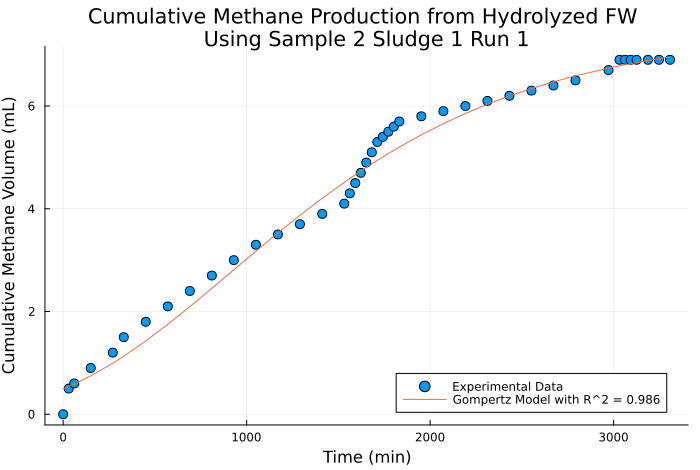
\includegraphics[width=.9\linewidth]{../plots/BMPs/Hydrolyzed FW/methane_kinetics_hydrolysate_2_s1_r1_min.png}
\end{center}

\begin{center}
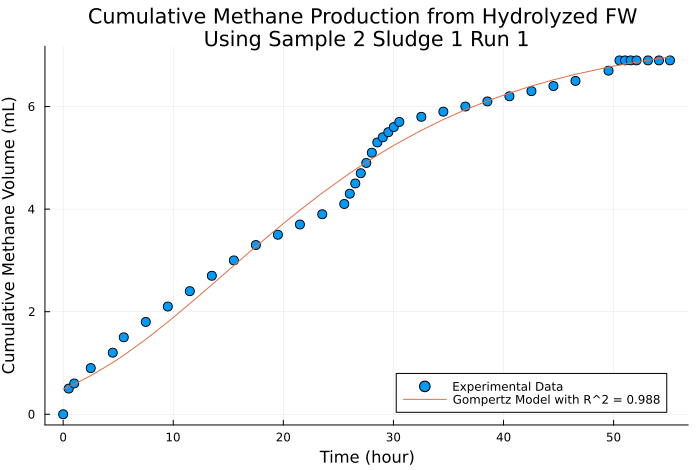
\includegraphics[width=.9\linewidth]{../plots/BMPs/Hydrolyzed FW/methane_kinetics_hydrolysate_2_s1_r1_hour.png}
\end{center}

\subsection{Sample 4}
\label{sec:org954e793}
Το δείγμα 4 ήταν αυτό με τα 4 ml mix στην υδρόλυση. Είναι η μέγιστη ποσότητα που χρησιμοποιήθηκε για τα πειράματα χώνευσης καθώς το 8 ml δεν είχε ιδιαίτερα μεγάλη διαφορά και είναι πολύ πιο ακριβό. Όπως προαναφέρθηκε, αναμένουμε να έχει παρόμοια ποιότητα με το 2 ml καθώς με εξαίρεση μίας ποσότητας γαλακτικού είναι σχεδόν ίδια.

\textbf{hydrolysate\textsubscript{4}\textsubscript{s1}\textsubscript{r1}}
\begin{minted}[breaklines=true,breakanywhere=true]{julia}

### Data Analysis on Hydrolysate with 4 ml ###

<<date_saving_fw_s1_r1>>

inds = 5:40
exp_meth_vol = [0, 13, 0.1, 0.2, 0.1, 0.2, 0.5, 1, 0.4, 0.1, 0.3, 0.1, 0.1, 0.1, 0.0, 0.0, 0.0, 0.05, 0.05, 0.05, 0.05, 0.05, 0.05, 0.05, 0.05, 0.05, 0.2, 0.2, 0.2, 0.1, 0, 0, 0, 0, 0, 0]
meth_vol_hydro_4 = cumsum(exp_meth_vol)[end]
exp_name = "hydrolysate_4_s1_r1"
source = "Hydrolyzed FW"
sample = "Sample 4"
sludge = "Sludge 1"
run_num = "Run 1"

input_cod = 0.1

<<bmp_data_processing>>

p0 = [170.0, 150.0, 1.0]
<<bmp_curve_fitting_min>>
model_hydro_4_min = vcat(sample, model_params, r_squared)
<<bmp_data_plotting>>

p0 = [170.0, 1000.0, 0.1]
<<bmp_curve_fitting_hour>>
model_hydro_4_hour = vcat(sample, model_params, r_squared)
<<bmp_data_plotting>>
\end{minted}

\begin{verbatim}
sys:1: UserWarning: No data for colormapping provided via 'c'. Parameters 'vmin', 'vmax' will be ignored
sys:1: UserWarning: No data for colormapping provided via 'c'. Parameters 'vmin', 'vmax' will be ignored
sys:1: UserWarning: No data for colormapping provided via 'c'. Parameters 'vmin', 'vmax' will be ignored
sys:1: UserWarning: No data for colormapping provided via 'c'. Parameters 'vmin', 'vmax' will be ignored
sys:1: UserWarning: No data for colormapping provided via 'c'. Parameters 'vmin', 'vmax' will be ignored
sys:1: UserWarning: No data for colormapping provided via 'c'. Parameters 'vmin', 'vmax' will be ignored
"/home/vidianos/Documents/9o_εξάμηνο/Masters_Thesis/plots/BMPs/Hydrolyzed FW/methane_kinetics_hydrolysate_4_hour.png"
\end{verbatim}

\subsubsection{Results}
\label{sec:org452e8ec}
Το δείγμα αυτό είχε την ιδιαιτερότητα της μεγαλύτερης παραγωγής μεθανίου από όλα τα δείγματα σε αρκετά γρήγορο ρυθμό, κάτι που προβλέπεται καθώς ήταν και η συμπεριφορά της λάσπης του. Η παραγωγή 17.35 ml μεθανίου είναι το \(36.9 \%\) αυτής του οξικού οξέος. Το γεγονός ότι είναι το ίδιο ποσοστό με αυτό του 2 ml είναι αρκετά καλό.

Επίσης, η παραγωγή είναι περίεργη καθώς παράγονται 13 ml μέσα σε ένα λεπτό και μετά το σύστημα μπαίνει σε μία σχεδόν στάσιμη φάση όπου η παραγωγή μεθανίου έχει επιβραδυνθεί σημαντικά, αλλά συνεχίζει να παράγει κάποια μικρή ποσότητα μέχρι και τις 51 ώρες όπου σταμάτησε το πείραμα. Οπότε, το γεγονός ότι το μοντέλο που προβλέπεται είναι ένα με πάρα πολύ υψηλό ειδικό ρυθμό ανάπτυξης το οποίο φτάνει σε στάσιμη φάση στα πρώτα λεπτά είναι αναμενόμενο.

Όμως, σε αντίθεση με τα άλλα πειράματα, αυτό είναι σχεδόν ολόσωστο σαν ιδέα καθώς 51 ώρες δεν παρήγαγαν ούτε το μισό του πρώτου λεπτού, οπότε παρόλο που θα αναμέναμε λίγο περισσότερη καμπύλη και όχι την μορφη που προκύπτει (η οποία είναι ουσιαστικά μία κατακόρυφη και μία οριζόντια γραμμή), η εξίσωση αυτή προβλέπει σχετικά καλά την πραγματικότητα και το R\textsuperscript{2} είναι 0.865, το οποίο είναι η καλύτερη προσαρμογή που έχουμε δεί σε ένα από αυτά τα πειράματα. Ο ειδικός ρυθμός ανάπτυξης που έχει προβλεφθεί είναι \(162.84 \frac{ml}{g ~ sCOD \min } \text{ ή } 9732.61 \frac{ml}{g ~ sCOD ~ hour}\) το οποίο είναι τεράστια διαφορά σε σχέση με τα άλλα πειράματα, ακόμη και αν χρησιμοποιηθεί το μοντέλο τους με τον γρήγορο ρυθμό.

Όπως αναφέρθηκε όμως, η συμπεριφορά αυτή είναι αναμενόμενη καθώς η λάσπη στο δοχείο αυτό είχε αυτή την ιδιαιτερότητα από την τροφοδοσία με το οξικό (παρόλο που εδώ φάνηκε πολύ πιο έντονα). Βέβαια, αξίζει να αναφερθεί πως παρότι ο ρυθμός αναμένεται να είναι μεγάλος, η τιμή αυτή είναι σχεδόν διπλάσια από τον αντίστοιχο ειδικό ρυθμό ανάπτυξης για τροφοδοσία με οξικό, το οποίο είναι αρκετά περίεργο.

\begin{center}
\begin{tabular}{lrrrr}
Timestamp & Minutes & Hours & Methane\textsubscript{Volume} & Cumulative\textsubscript{Methane}\textsubscript{Volume}\\[0pt]
\hline
01/04\textsubscript{11}:13 & 0.0 & 0.0 & 0.0 & 0.0\\[0pt]
01/04\textsubscript{11}:14 & 0.9999 & 0.0167 & 13.0 & 13.0\\[0pt]
01/04\textsubscript{11}:15 & 2.0001 & 0.0333 & 0.1 & 13.1\\[0pt]
01/04\textsubscript{11}:21 & 8.4387 & 0.1406 & 0.2 & 13.3\\[0pt]
01/04\textsubscript{11}:52 & 38.7648 & 0.6461 & 0.1 & 13.4\\[0pt]
01/04\textsubscript{12}:22 & 68.7648 & 1.1461 & 0.2 & 13.6\\[0pt]
01/04\textsubscript{16}:52 & 338.7654 & 5.6461 & 0.5 & 14.1\\[0pt]
02/04\textsubscript{10}:54 & 1420.5761 & 23.6763 & 1.0 & 15.1\\[0pt]
02/04\textsubscript{12}:54 & 1540.5835 & 25.6764 & 0.4 & 15.5\\[0pt]
02/04\textsubscript{13}:24 & 1570.5834 & 26.1764 & 0.1 & 15.6\\[0pt]
02/04\textsubscript{13}:54 & 1600.5837 & 26.6764 & 0.3 & 15.9\\[0pt]
02/04\textsubscript{14}:24 & 1630.5837 & 27.1764 & 0.1 & 16.0\\[0pt]
02/04\textsubscript{14}:54 & 1660.5836 & 27.6764 & 0.1 & 16.1\\[0pt]
02/04\textsubscript{15}:24 & 1690.5835 & 28.1764 & 0.1 & 16.2\\[0pt]
02/04\textsubscript{15}:54 & 1720.5835 & 28.6764 & 0.0 & 16.2\\[0pt]
02/04\textsubscript{16}:24 & 1750.5837 & 29.1764 & 0.0 & 16.2\\[0pt]
02/04\textsubscript{16}:54 & 1780.5838 & 29.6764 & 0.0 & 16.2\\[0pt]
02/04\textsubscript{17}:24 & 1810.5835 & 30.1764 & 0.05 & 16.25\\[0pt]
02/04\textsubscript{17}:54 & 1840.5902 & 30.6765 & 0.05 & 16.3\\[0pt]
02/04\textsubscript{19}:54 & 1960.5908 & 32.6765 & 0.05 & 16.35\\[0pt]
02/04\textsubscript{21}:54 & 2080.5924 & 34.6765 & 0.05 & 16.4\\[0pt]
02/04\textsubscript{23}:54 & 2200.5966 & 36.6766 & 0.05 & 16.45\\[0pt]
03/04\textsubscript{01}:54 & 2320.5967 & 38.6766 & 0.05 & 16.5\\[0pt]
03/04\textsubscript{03}:54 & 2440.5965 & 40.6766 & 0.05 & 16.55\\[0pt]
03/04\textsubscript{05}:54 & 2560.6014 & 42.6767 & 0.05 & 16.6\\[0pt]
03/04\textsubscript{07}:54 & 2680.6034 & 44.6767 & 0.05 & 16.65\\[0pt]
03/04\textsubscript{09}:54 & 2800.6034 & 46.6767 & 0.2 & 16.85\\[0pt]
03/04\textsubscript{12}:54 & 2980.6123 & 49.6769 & 0.2 & 17.05\\[0pt]
03/04\textsubscript{13}:54 & 3040.6122 & 50.6769 & 0.2 & 17.25\\[0pt]
03/04\textsubscript{14}:24 & 3070.6131 & 51.1769 & 0.1 & 17.35\\[0pt]
03/04\textsubscript{14}:54 & 3101.3718 & 51.6895 & 0.0 & 17.35\\[0pt]
03/04\textsubscript{15}:26 & 3133.4176 & 52.2236 & 0.0 & 17.35\\[0pt]
03/04\textsubscript{16}:29 & 3195.6885 & 53.2615 & 0.0 & 17.35\\[0pt]
03/04\textsubscript{17}:29 & 3255.693 & 54.2615 & 0.0 & 17.35\\[0pt]
03/04\textsubscript{18}:29 & 3315.6929 & 55.2615 & 0.0 & 17.35\\[0pt]
03/04\textsubscript{20}:29 & 3435.693 & 57.2615 & 0.0 & 17.35\\[0pt]
\end{tabular}
\end{center}

\begin{center}
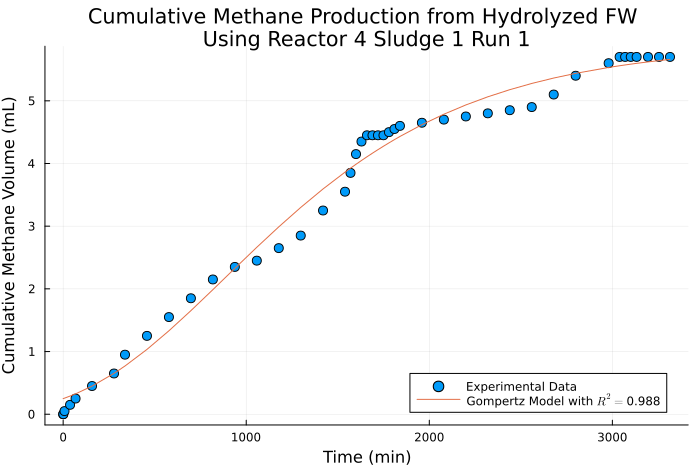
\includegraphics[width=.9\linewidth]{../plots/BMPs/Hydrolyzed FW/methane_kinetics_hydrolysate_4_s1_r1_min.png}
\end{center}

\begin{center}
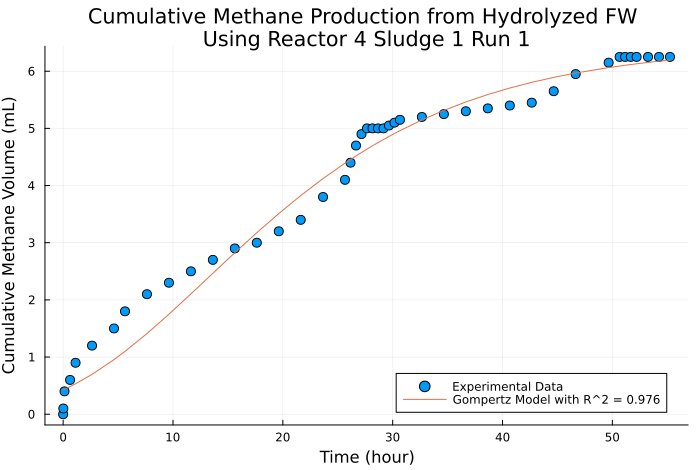
\includegraphics[width=.9\linewidth]{../plots/BMPs/Hydrolyzed FW/methane_kinetics_hydrolysate_4_s1_r1_hour.png}
\end{center}

\subsection{Untreated FW}
\label{sec:orgb0c4b60}
Εκτός από τα παραπάνω, σε ένα από τα δοχεία προστέθηκε ανεπεξέργαστο FW. Αυτό έχει διαφορά από το δείγμα 0, καθώς εκείνο υπέστει ζύμωση κατά τις 72 ώρες που ήταν στους 40 \(^oC\) ακόμη και χωρίς να προσθέσουμε κάποιο εμβόλιο, ενώ το δείγμα αυτό αναφέρεται σε food waste το οποίο δεν έχει υποστεί καμία επεξεργασία. Θα θέλαμε το δείγμα αυτό να έχει το χειρότερο performance (είτε πολύ αργή παραγωγή, ή μικρή τελική παραγωγή), το οποίο θα μας επιδείκνυε πως η επεξεργασία που έγινε βοηθάει πραγματικά στην χώνευση. Βέβαια, αξίζει να αναφερθεί πως το δοχείο αυτό είχε κάποιο προβλήματα με διαρροή στα αρχικά στάδια του πειράματος, οπότε ενδέχεται τα αποτελέσματα που θα προκύψουν να μην είναι έγκυρα. Παρακάτω φαίνεται ο κώδικας επεξεργασίας των αποτελεσμάτων του.

\textbf{untreated\textsubscript{fw}\textsubscript{s1}\textsubscript{r1}}
\begin{minted}[breaklines=true,breakanywhere=true]{julia}

### Data Analysis on Untreated FW ###

<<date_saving_fw_s1_r1>>

inds = 12:40
exp_meth_vol = [0, 0.2, 0, 0.1, 0.1, 0, 0, 0, 0.1, 0.1, 0, 0.1, 0.2, 0.1, 0.1, 0.1, 0.0, 0.1, 0.2, 0.1, 0.2, 0.1, 0.1, 0, 0, 0, 0, 0, 0]
meth_vol_hydro_fw = cumsum(exp_meth_vol)[end]
exp_name = "untreated_fw_s1_r1"
source = "Untreated FW"
sample = "FW 1"
sludge = "Sludge 1"
run_num = "Run 1"

input_cod = 0.1

<<bmp_data_processing>>

p0 = [20.0, 0.01, 1.0]
<<bmp_curve_fitting_min>>
model_hydro_fw_min = vcat(sample, model_params, r_squared)
<<bmp_data_plotting>>

p0 = [20.0, 1.0, 0.1]
<<bmp_curve_fitting_hour>>
model_hydro_fw_hour = vcat(sample, model_params, r_squared)
<<bmp_data_plotting>>
\end{minted}

\begin{verbatim}
"/home/vidianos/Documents/9o_εξάμηνο/Masters_Thesis/plots/BMPs/Untreated FW/methane_kinetics_untreated_fw_1_hour.png"
\end{verbatim}

\subsubsection{Results}
\label{sec:orgc2f7152}
Το δείγμα αυτό παρήγαγε μόνο το \(7.1 \%\) του μεθανίου που είχε παράξει από οξικό και το έκανε αυτό σε έναν αργό σχετικά ρυθμό. Κρίνεται πιθανό να μην επιλύθηκαν τα προβλήματα διαρροής που είχε και η παραγωγή του αερίου να ήταν στην πραγματικότητα μεγαλύτερη. Όμως όπως και στο δείγμα με 0 ml ένζυμα το οποίο όμως υπέστει 3 μέρες υδρόλυση και ζύμωση, μας "βολεύει" τα ποσοστά αυτά να είναι πολύ χαμηλά επειδή σημαίνει πως η επεξεργασία που κάναμε όντως συνείσφερε στην παραγωγή μεθανίου.

Από άποψη προσαρμογής, το μοντέλο Gompertz μπορεί να προσαρμοστεί πολύ καλά σε τέτοια δεδομένα όπου η παραγωγή μεθανίου γίνεται σε παρόμοιο ρυθμό για όλη την διεργασία. Το μοντέλο που θα αντιστοιχήσει θα είναι ένα μοντέλο χαμηλού ρυθμού (με βάση την παραπάνω διάκριση), το οποίο όμως είναι το μόνο που μπορεί να ισχύει καθώς στην αρχή δεν υπάρχει μία απότομη παραγωγή αερίου ταχύτατα για να μπορεί να προσαρμοστεί κάτι διαφορετικό. Τα μοντέλα σε λεπτά και ώρες δεν προσαρμόζονται με τον ακριβώς ίδιο τρόπο, αλλά οι διαφορές τους είναι μικρές. Ο ειδικός ρυθμός ανάπτυξης είναι της τάξης του \(0.0137 \frac{ml}{g ~ sCOD \min} \text{ ή } 0.823 \frac{ml}{g ~ sCOD ~ hour}\). Τα άλλα μοντέλα που προσαρμόστηκαν με αργό ρυθμό ανάπτυξης είχαν κινητικές της τάξης του 0.03-0.05 \(\frac{ml}{g ~ sCOD \min }\) οπότε αυτό είναι πιο αργό αλλά συγκρίσιμο με εκείνα.

\begin{center}
\begin{tabular}{lrrrr}
Timestamp & Minutes & Hours & Methane\textsubscript{Volume} & Cumulative\textsubscript{Methane}\textsubscript{Volume}\\[0pt]
\hline
02/04\textsubscript{10}:54 & 0.0 & 0.0 & 0.0 & 0.0\\[0pt]
02/04\textsubscript{12}:54 & 120.0074 & 2.0001 & 0.2 & 0.2\\[0pt]
02/04\textsubscript{13}:24 & 150.0073 & 2.5001 & 0.0 & 0.2\\[0pt]
02/04\textsubscript{13}:54 & 180.0076 & 3.0001 & 0.1 & 0.3\\[0pt]
02/04\textsubscript{14}:24 & 210.0076 & 3.5001 & 0.1 & 0.4\\[0pt]
02/04\textsubscript{14}:54 & 240.0075 & 4.0001 & 0.0 & 0.4\\[0pt]
02/04\textsubscript{15}:24 & 270.0074 & 4.5001 & 0.0 & 0.4\\[0pt]
02/04\textsubscript{15}:54 & 300.0073 & 5.0001 & 0.0 & 0.4\\[0pt]
02/04\textsubscript{16}:24 & 330.0076 & 5.5001 & 0.1 & 0.5\\[0pt]
02/04\textsubscript{16}:54 & 360.0076 & 6.0001 & 0.1 & 0.6\\[0pt]
02/04\textsubscript{17}:24 & 390.0073 & 6.5001 & 0.0 & 0.6\\[0pt]
02/04\textsubscript{17}:54 & 420.0141 & 7.0002 & 0.1 & 0.7\\[0pt]
02/04\textsubscript{19}:54 & 540.0146 & 9.0002 & 0.2 & 0.9\\[0pt]
02/04\textsubscript{21}:54 & 660.0162 & 11.0003 & 0.1 & 1.0\\[0pt]
02/04\textsubscript{23}:54 & 780.0205 & 13.0003 & 0.1 & 1.1\\[0pt]
03/04\textsubscript{01}:54 & 900.0205 & 15.0003 & 0.1 & 1.2\\[0pt]
03/04\textsubscript{03}:54 & 1020.0203 & 17.0003 & 0.0 & 1.2\\[0pt]
03/04\textsubscript{05}:54 & 1140.0253 & 19.0004 & 0.1 & 1.3\\[0pt]
03/04\textsubscript{07}:54 & 1260.0272 & 21.0005 & 0.2 & 1.5\\[0pt]
03/04\textsubscript{09}:54 & 1380.0273 & 23.0005 & 0.1 & 1.6\\[0pt]
03/04\textsubscript{12}:54 & 1560.0362 & 26.0006 & 0.2 & 1.8\\[0pt]
03/04\textsubscript{13}:54 & 1620.036 & 27.0006 & 0.1 & 1.9\\[0pt]
03/04\textsubscript{14}:24 & 1650.037 & 27.5006 & 0.1 & 2.0\\[0pt]
03/04\textsubscript{14}:54 & 1680.7956 & 28.0133 & 0.0 & 2.0\\[0pt]
03/04\textsubscript{15}:26 & 1712.8415 & 28.5474 & 0.0 & 2.0\\[0pt]
03/04\textsubscript{16}:29 & 1775.1124 & 29.5852 & 0.0 & 2.0\\[0pt]
03/04\textsubscript{17}:29 & 1835.1168 & 30.5853 & 0.0 & 2.0\\[0pt]
03/04\textsubscript{18}:29 & 1895.1168 & 31.5853 & 0.0 & 2.0\\[0pt]
03/04\textsubscript{20}:29 & 2015.1168 & 33.5853 & 0.0 & 2.0\\[0pt]
\end{tabular}
\end{center}

\begin{center}
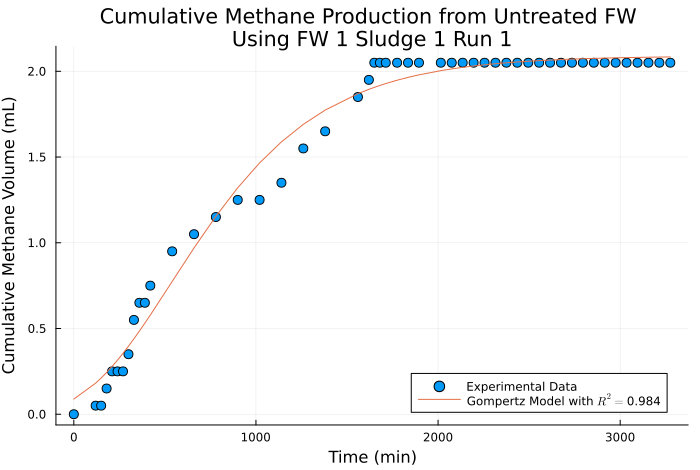
\includegraphics[width=.9\linewidth]{../plots/BMPs/Untreated FW/methane_kinetics_untreated_fw_s1_r1_min.png}
\end{center}

\begin{center}
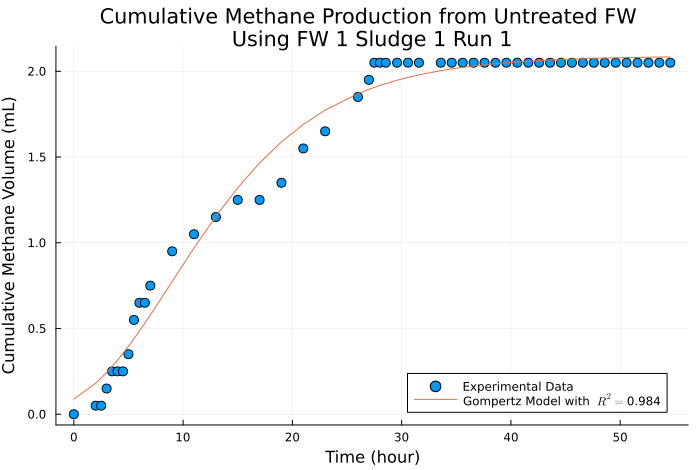
\includegraphics[width=.9\linewidth]{../plots/BMPs/Untreated FW/methane_kinetics_untreated_fw_s1_r1_hour.png}
\end{center}


\subsection{Update all}
\label{sec:orgba86b9a}
Όπως και παραπάνω για τα πειράματα στο οξικό, θα υπάρχει και ένα code block το οποίο θα κάνει update όλα τα code blocks, θα τα κάνει tangle σε ένα script file και θα αποθηκεύει ένα CSV με όλα τα κινητικά αποτελέσματα.

\textbf{update\textsubscript{hydrolysate}\textsubscript{tests}\textsubscript{s1}\textsubscript{r1}}
\begin{minted}[breaklines=true,breakanywhere=true]{julia}

<<hydrolysate_0_s1_r1>>
<<hydrolysate_1_s1_r1>>
<<hydrolysate_2_s1_r1>>
<<hydrolysate_4_s1_r1>>
<<untreated_fw_s1_r1>>

model_fit_table_min = Tables.table(vcat(reshape(model_hydro_0_min, 1, 5), reshape(model_hydro_1_min, 1, 5), reshape(model_hydro_2_min, 1, 5), reshape(model_hydro_4_min, 1, 5), reshape(model_hydro_fw_min, 1, 5)), header = [:Sample_Name, :Methane_Production_Potential, :Methane_Production_Rate, :Lag_Time, :R_squared])
CSV.write(datadir("exp_pro", "methane_from_hydrolysate_kinetics_min_s1_r1.csv"), model_fit_table_min)

model_fit_table_hour = Tables.table(vcat(reshape(model_hydro_0_hour, 1, 5), reshape(model_hydro_1_hour, 1, 5), reshape(model_hydro_2_hour, 1, 5), reshape(model_hydro_4_hour, 1, 5), reshape(model_hydro_fw_hour, 1, 5)), header = [:Sample_Name, :Methane_Production_Potential, :Methane_Production_Rate, :Lag_Time, :R_squared])
CSV.write(datadir("exp_pro", "methane_from_hydrolysate_kinetics_hour_s1_r1.csv"), model_fit_table_hour)
\end{minted}

Στα παρακάτω tables φαίνοντια οι κινητικές που προέκυψαν. Όπως έχει αναφερθεί και παραπάνω, έχουν προσαρμοστεί δύο μοντέλα στα περισσότερα, ένα αργό (το οποίο προσαρμόζει καλά την 2η και 3η μέρα) και ένα γρήγορο (το οποίο προσαρμόζει καλά στην αρχή του πειράματος). Το αργό μοντέλο φαίνεται στο timescale ωρών (ήταν πιο εύκολο να προσαρμοστεί εδώ επειδή για να βγεί στα λεπτά ήθελε initial condition ρυθμού σχεδόν 0) ενώ το γρήγορο φαίνεται στο timescale λεπτών. Αξίζει να σημειωθεί πως το δείγμα 4 δεν έχει καλή προσαρμογή σε αργό μοντέλο και το δείγμα FW δεν έχει καλή προσαρμογή σε γρήγορο. 

\begin{table}[htbp]
\caption{Kinetics with timescale in hours}
\centering
\begin{tabular}{lrrrr}
Sample\textsubscript{Name} & Production\textsubscript{Potential} & Production\textsubscript{Rate} & Lag\textsubscript{Time} & R\textsubscript{squared}\\[0pt]
Sample 0 & 65.137 & 1.666 & 0.0 & 0.884\\[0pt]
Sample 1 & 147.0709 & 3.279 & 0.0 & 0.843\\[0pt]
Sample 2 & 886.767 & 1.684 & 0.0 & 0.687\\[0pt]
Sample 4 & 161.139 & 9333.985 & 0.00164 & 0.839\\[0pt]
FW 1 & 22.964 & 0.812 & 0.0 & 0.984\\[0pt]
\end{tabular}
\end{table}

\begin{table}[htbp]
\caption{Kinetics with timescale in minutes}
\centering
\begin{tabular}{lrrrr}
Sample\textsubscript{Name} & Production\textsubscript{Potential} & Production\textsubscript{Rate} & Lag\textsubscript{Time} & R\textsubscript{squared}\\[0pt]
\hline
Sample 0 & 52.998 & 0.375 & 0.0 & 0.837\\[0pt]
Sample 1 & 110.589 & 0.817 & 0.0 & 0.693\\[0pt]
Sample 2 & 97.625 & 15.351 & 2.415 & 0.677\\[0pt]
Sample 4 & 161.135 & 156.195 & 0.0995 & 0.839\\[0pt]
FW 1 & 23.688 & 0.0128 & 0.0 & 0.982\\[0pt]
\end{tabular}
\end{table}


\subsection{Plotting Methane Potential}
\label{sec:org4ec2369}
Σε αυτό το section θα γίνει ένα plot το οποίο θα συγκρίνει μέγιστο μεθάνιο (παραγωγή από οξικό) με αυτό που παράχθηκε από το FW. Το plotting θα γίνει μέσω του \texttt{CairoMakie.jl} το οποίο είναι αρκετά featureful. Η διαδικασία είναι πως βάζουμε όλους τους όγκους παραγόμενου μεθανίου σε ένα vector και εκτός από την απόλυτη τιμή, υπολογίζουμε και το ποσοστό του μέγιστου που πετυχαίνει το υδρόλυμα. Όπως έχουν αποθηκευτεί, αυτό είναι διαίρεση του στοιχείου i+5 με το i. Έπειτα φτιάχνουμε ένα string των ποσοστών αυτών μαζί με τα labels που τους αντιστοιχούν. Αυτό θα προστεθεί στο plot που φτιάχνουμε.

Έχοντας κάνει το preprocessing αυτό, ξεκινάμε την δημιουργία διαγραμμάτων. Φτιάχνουμε ένα figure και έναν άξονα πάνω σε αυτό όπου θα κάνουμε τα bar plots που θέλουμε. Οι μεταβλητές \texttt{xdata} και \texttt{grp} είναι απαραίτητες για να φτιαχτεί το plot. Το xdata λέει σε ποιό σημείο του άξονα x θα πάει κάθε δεδομένο (όπως τα έχουμε ορίσει θα είναι από το 1 εώς το 5 δύο φορές) ενώ το grp λέει σε ποιό group θα ανήκει το κάθε πείραμα. Τα 5 πρώτα είναι στο group 1 (οξικό) ενώ τα άλλα στο 2 (υδρόλυμα). Ορίζουμε και το legend και το plot αυτό είναι έτοιμο. Από κάτω, κάνουμε insert το string με τα ποσοστά που υπολογίστηκε παραπάνω σε ένα text plot του Makie. Έπειτα, κάνουμε save το plot αυτό.

\begin{minted}[breaklines=true,breakanywhere=true]{julia}

using CairoMakie
colors = Makie.wong_colors()

meth_vol = [meth_vol_acet_0, meth_vol_acet_1, meth_vol_acet_2, meth_vol_acet_4, meth_vol_acet_fw, meth_vol_hydro_0, meth_vol_hydro_1, meth_vol_hydro_2, meth_vol_hydro_4, meth_vol_hydro_fw]

percent_bmp = [meth_vol[i+5]/meth_vol[i] for i in 1:5]
string_bmp = vcat(string.(round.(percent_bmp.*100, digits = 2)).*" %", ["0 ml", "1 ml", "2 ml", "4 ml", "Untreated \nFW"])

fig = Figure(size = (600, 400))
ax = Axis(fig[1,1], xticks = (1:5, ["0 ml", "1 ml", "2 ml", "4 ml", "Untreated FW"]),
          title = "Acetate vs Hydrolysate BMP")

xdata = [1, 2, 3, 4, 5, 1, 2, 3, 4, 5]
grp = [1, 1, 1, 1, 1, 2, 2, 2, 2, 2]

barplot!(ax, xdata, meth_vol,
        dodge = grp,
        color = colors[grp])

# Legend
labels = ["Acetate", "FW Hydrolysate"]
elements = [PolyElement(polycolor = colors[i]) for i in 1:length(labels)]
title = "Source"
Legend(fig[1,2], elements, labels, title)

ax2 = Axis(fig[2, 1], xticks = (1:5, ["0 ml", "1 ml", "2 ml", "4 ml", "Untreated FW"]), yticks = ([1, 2], ["", ""]), title = "% of Acetate BMP in Hydrolysates")
hidespines!(ax2)
hidedecorations!(ax2)
text!(xdata, repeat(1:1, 10), text = string_bmp, align = [(:left, :top), (:left, :top), (:center, :top), (:right, :top), (:right, :top), (:left, :bottom), (:left, :bottom), (:center, :bottom), (:right, :bottom), (:right, :bottom)])

save(plotsdir("BMPs", "Hydrolyzed FW", "acet_vs_hydro_bmp_"*comp_name*".png"), fig)
\end{minted}

Για να τρέξουμε αυτό το code block χωρίς προβλήματα, πρέπει να δώσουμε τιμή στο \texttt{comp\_name} και να κάνουμε update τα tests ώστε να έχουμε τα σωστά.
\begin{minted}[breaklines=true,breakanywhere=true]{julia}

<<update_acetate_tests_s1>>
<<update_hydrolysate_tests_s1_r1>>

comp_name = "s1_r1"
<<BMP_plotting>>
\end{minted}

\begin{center}
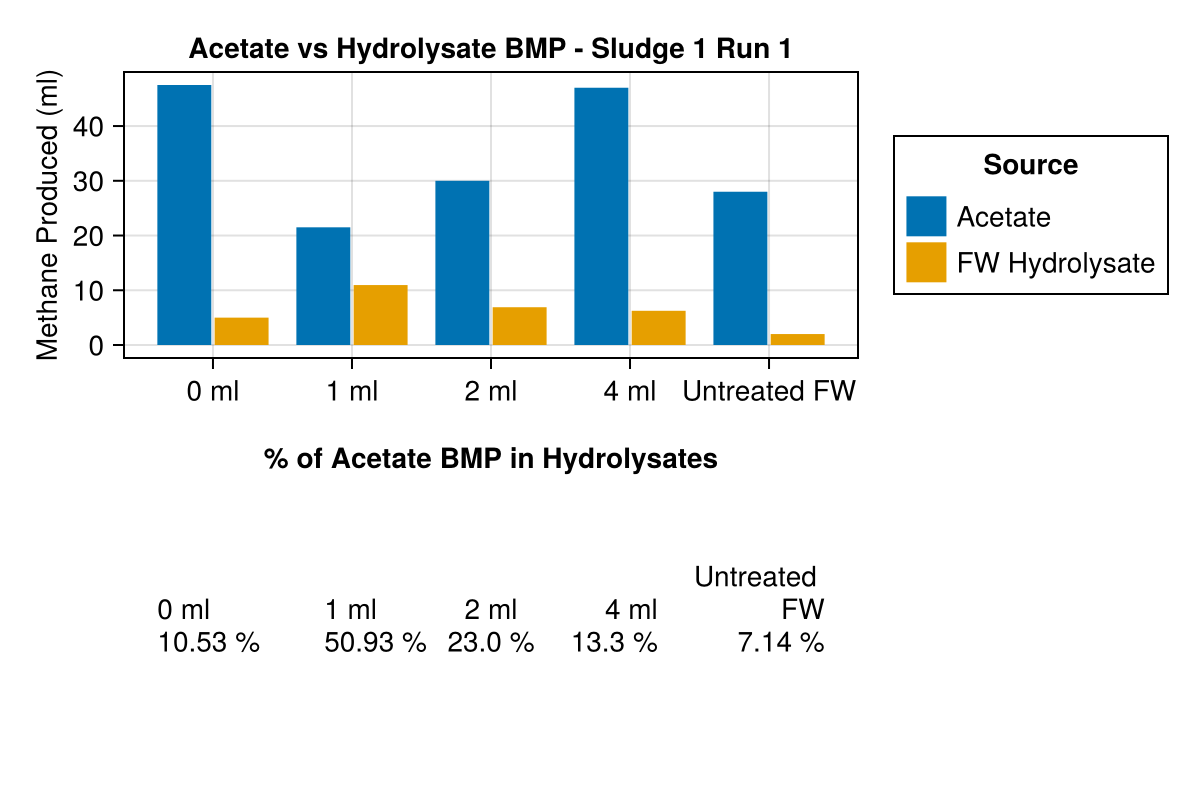
\includegraphics[width=.9\linewidth]{../plots/BMPs/Hydrolyzed FW/acet_vs_hydro_bmp_s1_r1.png}
\end{center}

\subsection{Συμπεράσματα του πειραματικού κύκλου αυτού}
\label{sec:orgbfd302b}
Το πείραμα αυτό ήταν το πρώτο πείραμα όπου τροφοδοτήσαμε με υδρολύματα από FW για να δούμε την απόκριση του συστήματος σε αυτά.

Η σημαντικότερη παρατήρηση που μπορεί να γίνει είναι η ανομοιογένεια στον ρυθμό. Τα πρώτα λεπτά μετά την προσθήκη του υποστρώματος υπήρξε ταχεία παραγωγή αερίου ενώ μετά ο ρυθμός επιβράδυνε σημαντικά και για τις επόμενες 2 ημέρες παραγόταν αέριο. Έτσι, υπήρχε το φαινόμενο όπου από διαφορετικές αρχικές συνθήκες, μπορούσαμε να προσαρμώσουμε 2 μοντέλα Gompertz στο σύστημα. Το ένα έχει έναν γρήγορο ρυθμό ανάπτυξης και ταιριάζει τέλεια στην αρχή του πειράματος ενώ το άλλο έχει πολύ αργό ρυθμό και ταιριάζει στο τελείωμα της αντίδρασης όπου ο ρυθμός είναι αργός. Αυτό δημιουργεί την υπόνοια ότι κάτι συμβαίνει στο σύστημα και αλλάζει ο μηχανισμός της αντίδρασης. Περισσότερα πάνω σε αυτή την υπόθεση θα αναφερθούν παρακάτω.

Εκτός από τους ρυθμούς αυτούς, αξίζει να σημειωθεί πως κανένα από τα μοντέλα δεν είχε σημαντικό lag time. Αυτό είχε παρατηρηθεί και στα πειράματα με το οξικό. Γενικά, το lag time είναι μία φυσική παράμετρος του συστήματος που εκφράζει πόσο γρήγορα αντιδρά το σύστημα με μία αλλαγή στο περιβάλλον του. Για την προσθήκη οξικού είναι λογικό το μηδενικό lag time καθώς είναι το ιδανικό υπόστρωμα του συστήματος. Για το υδρόλυμα, αυτό δεν αναμένεται.

Ως προς το biomethane potential (BMP) του συστήματος, όπως θα αναμενόταν τα υδρολύματα παρήγαγαν λιγότερο μεθάνιο από το οξικό. Το δείγμα με 0 ml παρήγαγε το λιγότερο μεθάνιο αναλογικά με το πείραμα οξικού στο δοχείο αυτό. Ακολουθήθηκε από το 2 και 4 ml τα οποία είχαν το ίδιο ποσοστό μεθανίου αναλογικά με το οξικό τους ενώ το μέγιστο ποσοστό ήταν από το 1 ml \(( 60.7 \% )\). Στις μετρήσεις COD, το δείγμα αυτό είχε πολύ μεγάλο sCOD, το οποίο μπορεί να σημαίνει πως είχε πολύ καλή διαλυτοποίηση το οποίο να οδήγησε σε καλύτερη παραγωγή μεθανίου. Για το ανεπεξέργαστο FW, υπάρχει η σκέψη πως υπήρχε διαρροή, καθώς δεν είχε το φαινόμενο του γρήγορου ρυθμού στην αρχή και η συνολική παραγωγικότητα ήταν πολύ χαμηλή.

Λόγω των προβλημάτων που παρουσιάστηκαν και για να επιβεβαιώσουμε αν είναι επαναλήψιμα αυτά, έγινε και ένα δεύτερο πείραμα με τις ίδιες συνθήκες για να δούμε τα αποτελέσματα του.

\section{FW Hydrolysate S1\textsubscript{R2} Processing}
\label{sec:org8c73206}
Στο section αυτό θα αναλυθούν τα αποτελεσματα του δεύτερου πειράματος που χρησιμοποιήσε FW hydrolysate ως υπόστρωμα (S1\textsubscript{R2} επειδή είναι το δεύτερο run με την πρώτη λάσπη). Βρίσκεται σε πλήρη αντιστοιχία με το προηγούμενο πείραμα και έγινε για επαναληψιμότητα. Οπότε, σκοπός είναι να εξετάσουμε αν είναι παρόμοιο με το προηγούμενο ή αν διαφέρει σημαντικά και στην περίπτωση του 2ου, να κρίνουμε ποιά από τις δύο περιπτώσεις είναι πραγματικά ο outlier. Τα σχόλια για το τι είναι κάθε δείγμα θα μείνουν ίδια με παραπάνω για υπενθύμιση.

\subsection{Sample 0}
\label{sec:org9749823}
Το δείγμα αυτό είναι labelled ως δείγμα 0 καθώς είναι το δείγμα το οποίο τροφοδοτήθηκε με treated FW, όμως χωρίς προσθήκη του μιξ ενζύμων και μικροοργανισμών. Όπως έχουμε δεί, όλες οι αντιδράσεις που γίνονται κατά την υδρόλυση και ζύμωση μπορούν να γίνουν και χωρίς το μιξ. Όμως, γινόντουσαν πιο αποτελεσματικά με την προσθήκη αυτού. Οπότε, ελπίζουμε πως το δείγμα αυτό θα έχει χειρότερα αποτελέσματα από τα άλλα, το οποίο θα μας οδηγήσει στην υπόθεση ότι το μιξ βελτιώνει όχι μόνο τα κριτήρια υδρόλυσης και οξεογένεσης αλλά και αυτό της μεθανογένεσης.

\textbf{hydrolysate\textsubscript{0}\textsubscript{s1}\textsubscript{r2}}
\begin{minted}[breaklines=true,breakanywhere=true]{julia}

### Data Analysis on Hydrolysate with 0 ml ###

<<date_saving_fw_s1_r2>>

inds = 1:69
exp_meth_vol = [0, 0, 0, 0, 0, 0, 0, 0.1, 0.1, 0.1, 0.05, 0.1, 0.1, 0.05, 0.1, 0.1, 0.1, 0.1, 0.1, 0.05, 0.1, 0.1, 0.1, 0.1, 0.1, 0.1, 0, 0, 0, 0, 0, 0, 0, 0, 0.1, 0.1, 0.1, 0.1, 0.05, 0.05, 0.1, 0.05, 0, 0, 0.05, 0.05, 0.05, 0.1, 0.05, 0.05, 0.05, 0.05, 0.1, 0.1, 0.1, 0.05, 0.05, 0.05, 0.05, 0, 0.05, 0, 0.02, 0.02, 0.01, 0, 0, 0, 0]
meth_vol_hydro_0 = cumsum(exp_meth_vol)[end]

exp_name = "hydrolysate_0_s1_r2"
source = "Hydrolyzed FW"
sample = "Sample 0"
sludge = "Sludge 1"
run_num = "Run 2"
input_cod = 0.1

<<bmp_data_processing>>

# The same model is fit either with min or hour
p0 = [50.0, 0.4, 1.0]
<<bmp_curve_fitting_min>>
model_hydro_0_min = vcat(sample, model_params, r_squared)
<<bmp_data_plotting>>

p0 = [40.0, 1.0, 1.0]
<<bmp_curve_fitting_hour>>
model_hydro_0_hour = vcat(sample, model_params, r_squared)
<<bmp_data_plotting>>
\end{minted}

\subsubsection{Results}
\label{sec:orgb2aed18}
Παρακάτω φαίνονται τα αποτελέσματα του σχετικού πειράματος.

\begin{center}
\begin{tabular}{lrrrr}
Timestamp & Minutes & Hours & Methane\textsubscript{Volume} & Cumulative\textsubscript{Methane}\textsubscript{Volume}\\[0pt]
\hline
03/04\textsubscript{14}:37 & 0.0 & 0.0 & 0.0 & 0.0\\[0pt]
03/04\textsubscript{14}:45 & 8.4249 & 0.1404 & 0.0 & 0.0\\[0pt]
03/04\textsubscript{14}:51 & 14.5619 & 0.2427 & 0.0 & 0.0\\[0pt]
03/04\textsubscript{14}:56 & 19.6074 & 0.3268 & 0.0 & 0.0\\[0pt]
03/04\textsubscript{15}:29 & 51.8783 & 0.8646 & 0.0 & 0.0\\[0pt]
03/04\textsubscript{16}:29 & 111.8786 & 1.8646 & 0.0 & 0.0\\[0pt]
03/04\textsubscript{17}:29 & 171.8831 & 2.8647 & 0.0 & 0.0\\[0pt]
03/04\textsubscript{18}:29 & 231.883 & 3.8647 & 0.1 & 0.1\\[0pt]
03/04\textsubscript{20}:29 & 351.8831 & 5.8647 & 0.1 & 0.2\\[0pt]
03/04\textsubscript{22}:29 & 471.8831 & 7.8647 & 0.1 & 0.3\\[0pt]
04/04\textsubscript{00}:29 & 591.8898 & 9.8648 & 0.05 & 0.35\\[0pt]
04/04\textsubscript{02}:29 & 711.8898 & 11.8648 & 0.1 & 0.45\\[0pt]
04/04\textsubscript{04}:29 & 831.8898 & 13.8648 & 0.1 & 0.55\\[0pt]
04/04\textsubscript{06}:29 & 951.8898 & 15.8648 & 0.05 & 0.6\\[0pt]
04/04\textsubscript{08}:29 & 1071.8939 & 17.8649 & 0.1 & 0.7\\[0pt]
04/04\textsubscript{10}:29 & 1191.8998 & 19.865 & 0.1 & 0.8\\[0pt]
04/04\textsubscript{12}:29 & 1311.9002 & 21.865 & 0.1 & 0.9\\[0pt]
04/04\textsubscript{14}:29 & 1431.9003 & 23.865 & 0.1 & 1.0\\[0pt]
04/04\textsubscript{16}:29 & 1551.9002 & 25.865 & 0.1 & 1.1\\[0pt]
04/04\textsubscript{18}:29 & 1671.9187 & 27.8653 & 0.05 & 1.15\\[0pt]
04/04\textsubscript{20}:29 & 1791.9215 & 29.8654 & 0.1 & 1.25\\[0pt]
04/04\textsubscript{22}:29 & 1911.9228 & 31.8654 & 0.1 & 1.35\\[0pt]
05/04\textsubscript{00}:29 & 2031.9178 & 33.8653 & 0.1 & 1.45\\[0pt]
05/04\textsubscript{02}:29 & 2151.9188 & 35.8653 & 0.1 & 1.55\\[0pt]
05/04\textsubscript{04}:29 & 2271.9218 & 37.8654 & 0.1 & 1.65\\[0pt]
05/04\textsubscript{06}:29 & 2391.9224 & 39.8654 & 0.1 & 1.75\\[0pt]
05/04\textsubscript{08}:29 & 2511.9224 & 41.8654 & 0.0 & 1.75\\[0pt]
05/04\textsubscript{09}:29 & 2571.9221 & 42.8654 & 0.0 & 1.75\\[0pt]
05/04\textsubscript{10}:37 & 2640.1985 & 44.0033 & 0.0 & 1.75\\[0pt]
05/04\textsubscript{10}:38 & 2641.1985 & 44.02 & 0.0 & 1.75\\[0pt]
05/04\textsubscript{10}:39 & 2642.1984 & 44.0366 & 0.0 & 1.75\\[0pt]
05/04\textsubscript{10}:40 & 2643.1753 & 44.0529 & 0.0 & 1.75\\[0pt]
05/04\textsubscript{11}:40 & 2703.3506 & 45.0558 & 0.0 & 1.75\\[0pt]
05/04\textsubscript{12}:40 & 2763.3564 & 46.0559 & 0.0 & 1.75\\[0pt]
05/04\textsubscript{14}:40 & 2883.3563 & 48.0559 & 0.1 & 1.85\\[0pt]
05/04\textsubscript{16}:40 & 3003.3568 & 50.0559 & 0.1 & 1.95\\[0pt]
05/04\textsubscript{18}:40 & 3123.3627 & 52.056 & 0.1 & 2.05\\[0pt]
05/04\textsubscript{20}:40 & 3243.3636 & 54.0561 & 0.1 & 2.15\\[0pt]
05/04\textsubscript{22}:40 & 3363.3662 & 56.0561 & 0.05 & 2.2\\[0pt]
06/04\textsubscript{00}:40 & 3483.3698 & 58.0562 & 0.05 & 2.25\\[0pt]
06/04\textsubscript{02}:40 & 3603.3701 & 60.0562 & 0.1 & 2.35\\[0pt]
06/04\textsubscript{04}:40 & 3723.37 & 62.0562 & 0.05 & 2.4\\[0pt]
06/04\textsubscript{06}:40 & 3843.3753 & 64.0563 & 0.0 & 2.4\\[0pt]
06/04\textsubscript{08}:40 & 3963.3773 & 66.0563 & 0.0 & 2.4\\[0pt]
06/04\textsubscript{10}:40 & 4083.3773 & 68.0563 & 0.05 & 2.45\\[0pt]
06/04\textsubscript{12}:40 & 4203.3853 & 70.0564 & 0.05 & 2.5\\[0pt]
06/04\textsubscript{14}:40 & 4323.3855 & 72.0564 & 0.05 & 2.55\\[0pt]
06/04\textsubscript{16}:40 & 4443.3882 & 74.0565 & 0.1 & 2.65\\[0pt]
06/04\textsubscript{18}:40 & 4563.3888 & 76.0565 & 0.05 & 2.7\\[0pt]
06/04\textsubscript{20}:40 & 4683.3889 & 78.0565 & 0.05 & 2.75\\[0pt]
06/04\textsubscript{22}:40 & 4803.389 & 80.0565 & 0.05 & 2.8\\[0pt]
07/04\textsubscript{00}:40 & 4923.3992 & 82.0567 & 0.05 & 2.85\\[0pt]
07/04\textsubscript{02}:40 & 5043.3998 & 84.0567 & 0.1 & 2.95\\[0pt]
07/04\textsubscript{04}:40 & 5163.3999 & 86.0567 & 0.1 & 3.05\\[0pt]
07/04\textsubscript{06}:40 & 5283.3998 & 88.0567 & 0.1 & 3.15\\[0pt]
07/04\textsubscript{08}:40 & 5403.4018 & 90.0567 & 0.05 & 3.2\\[0pt]
07/04\textsubscript{10}:40 & 5523.4112 & 92.0569 & 0.05 & 3.25\\[0pt]
07/04\textsubscript{12}:40 & 5643.4132 & 94.0569 & 0.05 & 3.3\\[0pt]
07/04\textsubscript{14}:40 & 5763.4147 & 96.0569 & 0.05 & 3.35\\[0pt]
07/04\textsubscript{16}:40 & 5883.416 & 98.0569 & 0.0 & 3.35\\[0pt]
07/04\textsubscript{18}:40 & 6003.4222 & 100.057 & 0.05 & 3.4\\[0pt]
07/04\textsubscript{20}:40 & 6123.4235 & 102.0571 & 0.0 & 3.4\\[0pt]
07/04\textsubscript{22}:40 & 6243.4246 & 104.0571 & 0.02 & 3.42\\[0pt]
08/04\textsubscript{00}:40 & 6363.4417 & 106.0574 & 0.02 & 3.44\\[0pt]
08/04\textsubscript{02}:40 & 6483.4429 & 108.0574 & 0.01 & 3.45\\[0pt]
08/04\textsubscript{04}:40 & 6603.434 & 110.0572 & 0.0 & 3.45\\[0pt]
08/04\textsubscript{06}:40 & 6723.4333 & 112.0572 & 0.0 & 3.45\\[0pt]
08/04\textsubscript{08}:40 & 6843.4332 & 114.0572 & 0.0 & 3.45\\[0pt]
08/04\textsubscript{10}:40 & 6963.4332 & 116.0572 & 0.0 & 3.45\\[0pt]
\end{tabular}
\end{center}


\begin{center}
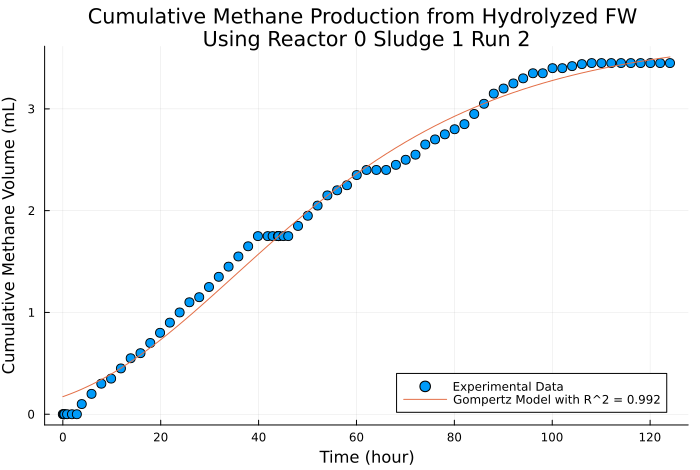
\includegraphics[width=.9\linewidth]{../plots/BMPs/Hydrolyzed FW/methane_kinetics_hydrolysate_0_s1_r2_hour.png}
\end{center}

\subsection{Sample 1}
\label{sec:org3f4b3ad}
Το δείγμα αυτό τροφοδοτήθηκε με το υδρόλυμα το οποίο είχε προσθήκη 1 ml mix. Στο αρχικό κινητικό πείραμα, το δείγμα αυτό είχε αρκετά παρόμοια συμπεριφορά με το 0 και χειρότερη αυτής του 1. Από την μέτρηση του COD του, είχε αναπάντεχα υψηλό sCOD. Αυτό σημαίνει είτε πως έγινε κάποιο λάθος στην ανάλυση ή ότι απλώς έγινε πολύ καλύτερη υδρόλυση από ότι περιμέναμε στο πείραμα αυτό. Με βάση το sCOD του, αναμένεται να έχει καλά αποτελέσματα. Με βάση την HPLC του αρχικού πειράματος, θα περιμέναμε να είναι λίγο καλύτερο από το 0.

\textbf{hydrolysate\textsubscript{1}\textsubscript{s1}\textsubscript{r2}}
\begin{minted}[breaklines=true,breakanywhere=true]{julia}

### Data Analysis on Hydrolysate with 1 ml ###

<<date_saving_fw_s1_r2>>

inds = 2:69
exp_meth_vol = [0, 0, 0, 0, 0, 0.2, 0.2, 0.2, 0.2, 0.2, 0.2, 0.2, 0.2, 0.2, 0.2, 0.2, 0.2, 0.2, 0.2, 0.2, 0.2, 0.05, 0.1, 0.2, 0.2, 0.2, 0.2, 0.1, 0.05, 0.1, 0, 0, 0, 0.1, 0.1, 0.2, 0.4, 0.5, 0.2, 0.1, 0.1, 0.2, 0, 0.1, 0.2, 0.2, 0.1, 0.3, 0.1, 0.1, 0, 0.1, 0.2, 0.2, 0.1, 0.2, 0.2, 0.1, 0.1, 0, 0.1, 0.2, 0, 0.1, 0.1, 0.2, 0.2, 0.1]
meth_vol_hydro_1 = cumsum(exp_meth_vol)[end]
exp_name = "hydrolysate_1_s1_r2"
source = "Hydrolyzed FW"
sample = "Sample 1"
sludge = "Sludge 1"
run_num = "Run 2"
input_cod = 0.1

p0 = [130.0, 10.0, 1.0]
<<bmp_data_processing>>
<<bmp_curve_fitting_min>>
model_hydro_1_min = vcat(sample, model_params, r_squared)
<<bmp_data_plotting>>

p0 = [200.0, 5.0, 1.0]
<<bmp_curve_fitting_hour>>
model_hydro_1_hour = vcat(sample, model_params, r_squared)
<<bmp_data_plotting>>
\end{minted}

\subsubsection{Results}
\label{sec:org5763445}
\begin{center}
\begin{tabular}{lrrrr}
Timestamp & Minutes & Hours & Methane\textsubscript{Volume} & Cumulative\textsubscript{Methane}\textsubscript{Volume}\\[0pt]
\hline
03/04\textsubscript{14}:45 & 0.0 & 0.0 & 0.0 & 0.0\\[0pt]
03/04\textsubscript{14}:51 & 6.137 & 0.1023 & 0.0 & 0.0\\[0pt]
03/04\textsubscript{14}:56 & 11.1825 & 0.1864 & 0.0 & 0.0\\[0pt]
03/04\textsubscript{15}:29 & 43.4534 & 0.7242 & 0.0 & 0.0\\[0pt]
03/04\textsubscript{16}:29 & 103.4538 & 1.7242 & 0.0 & 0.0\\[0pt]
03/04\textsubscript{17}:29 & 163.4582 & 2.7243 & 0.2 & 0.2\\[0pt]
03/04\textsubscript{18}:29 & 223.4582 & 3.7243 & 0.2 & 0.4\\[0pt]
03/04\textsubscript{20}:29 & 343.4582 & 5.7243 & 0.2 & 0.6\\[0pt]
03/04\textsubscript{22}:29 & 463.4582 & 7.7243 & 0.2 & 0.8\\[0pt]
04/04\textsubscript{00}:29 & 583.4649 & 9.7244 & 0.2 & 1.0\\[0pt]
04/04\textsubscript{02}:29 & 703.4649 & 11.7244 & 0.2 & 1.2\\[0pt]
04/04\textsubscript{04}:29 & 823.465 & 13.7244 & 0.2 & 1.4\\[0pt]
04/04\textsubscript{06}:29 & 943.4649 & 15.7244 & 0.2 & 1.6\\[0pt]
04/04\textsubscript{08}:29 & 1063.469 & 17.7245 & 0.2 & 1.8\\[0pt]
04/04\textsubscript{10}:29 & 1183.4749 & 19.7246 & 0.2 & 2.0\\[0pt]
04/04\textsubscript{12}:29 & 1303.4754 & 21.7246 & 0.2 & 2.2\\[0pt]
04/04\textsubscript{14}:29 & 1423.4755 & 23.7246 & 0.2 & 2.4\\[0pt]
04/04\textsubscript{16}:29 & 1543.4754 & 25.7246 & 0.2 & 2.6\\[0pt]
04/04\textsubscript{18}:29 & 1663.4938 & 27.7249 & 0.2 & 2.8\\[0pt]
04/04\textsubscript{20}:29 & 1783.4966 & 29.7249 & 0.2 & 3.0\\[0pt]
04/04\textsubscript{22}:29 & 1903.4979 & 31.725 & 0.2 & 3.2\\[0pt]
05/04\textsubscript{00}:29 & 2023.493 & 33.7249 & 0.05 & 3.25\\[0pt]
05/04\textsubscript{02}:29 & 2143.4939 & 35.7249 & 0.1 & 3.35\\[0pt]
05/04\textsubscript{04}:29 & 2263.4969 & 37.7249 & 0.2 & 3.55\\[0pt]
05/04\textsubscript{06}:29 & 2383.4976 & 39.725 & 0.2 & 3.75\\[0pt]
05/04\textsubscript{08}:29 & 2503.4975 & 41.725 & 0.2 & 3.95\\[0pt]
05/04\textsubscript{09}:29 & 2563.4972 & 42.725 & 0.2 & 4.15\\[0pt]
05/04\textsubscript{10}:37 & 2631.7736 & 43.8629 & 0.1 & 4.25\\[0pt]
05/04\textsubscript{10}:38 & 2632.7736 & 43.8796 & 0.05 & 4.3\\[0pt]
05/04\textsubscript{10}:39 & 2633.7736 & 43.8962 & 0.1 & 4.4\\[0pt]
05/04\textsubscript{10}:40 & 2634.7504 & 43.9125 & 0.0 & 4.4\\[0pt]
05/04\textsubscript{11}:40 & 2694.9257 & 44.9154 & 0.0 & 4.4\\[0pt]
05/04\textsubscript{12}:40 & 2754.9315 & 45.9155 & 0.0 & 4.4\\[0pt]
05/04\textsubscript{14}:40 & 2874.9314 & 47.9155 & 0.1 & 4.5\\[0pt]
05/04\textsubscript{16}:40 & 2994.9319 & 49.9155 & 0.1 & 4.6\\[0pt]
05/04\textsubscript{18}:40 & 3114.9378 & 51.9156 & 0.2 & 4.8\\[0pt]
05/04\textsubscript{20}:40 & 3234.9387 & 53.9156 & 0.4 & 5.2\\[0pt]
05/04\textsubscript{22}:40 & 3354.9413 & 55.9157 & 0.5 & 5.7\\[0pt]
06/04\textsubscript{00}:40 & 3474.945 & 57.9157 & 0.2 & 5.9\\[0pt]
06/04\textsubscript{02}:40 & 3594.9452 & 59.9158 & 0.1 & 6.0\\[0pt]
06/04\textsubscript{04}:40 & 3714.9451 & 61.9158 & 0.1 & 6.1\\[0pt]
06/04\textsubscript{06}:40 & 3834.9504 & 63.9158 & 0.2 & 6.3\\[0pt]
06/04\textsubscript{08}:40 & 3954.9524 & 65.9159 & 0.0 & 6.3\\[0pt]
06/04\textsubscript{10}:40 & 4074.9524 & 67.9159 & 0.1 & 6.4\\[0pt]
06/04\textsubscript{12}:40 & 4194.9604 & 69.916 & 0.2 & 6.6\\[0pt]
06/04\textsubscript{14}:40 & 4314.9606 & 71.916 & 0.2 & 6.8\\[0pt]
06/04\textsubscript{16}:40 & 4434.9633 & 73.9161 & 0.1 & 6.9\\[0pt]
06/04\textsubscript{18}:40 & 4554.964 & 75.9161 & 0.3 & 7.2\\[0pt]
06/04\textsubscript{20}:40 & 4674.9641 & 77.9161 & 0.1 & 7.3\\[0pt]
06/04\textsubscript{22}:40 & 4794.9641 & 79.9161 & 0.1 & 7.4\\[0pt]
07/04\textsubscript{00}:40 & 4914.9743 & 81.9162 & 0.0 & 7.4\\[0pt]
07/04\textsubscript{02}:40 & 5034.9749 & 83.9162 & 0.1 & 7.5\\[0pt]
07/04\textsubscript{04}:40 & 5154.975 & 85.9163 & 0.2 & 7.7\\[0pt]
07/04\textsubscript{06}:40 & 5274.9749 & 87.9162 & 0.2 & 7.9\\[0pt]
07/04\textsubscript{08}:40 & 5394.9769 & 89.9163 & 0.1 & 8.0\\[0pt]
07/04\textsubscript{10}:40 & 5514.9863 & 91.9164 & 0.2 & 8.2\\[0pt]
07/04\textsubscript{12}:40 & 5634.9883 & 93.9165 & 0.2 & 8.4\\[0pt]
07/04\textsubscript{14}:40 & 5754.9898 & 95.9165 & 0.1 & 8.5\\[0pt]
07/04\textsubscript{16}:40 & 5874.9911 & 97.9165 & 0.1 & 8.6\\[0pt]
07/04\textsubscript{18}:40 & 5994.9974 & 99.9166 & 0.0 & 8.6\\[0pt]
07/04\textsubscript{20}:40 & 6114.9986 & 101.9166 & 0.1 & 8.7\\[0pt]
07/04\textsubscript{22}:40 & 6234.9998 & 103.9167 & 0.2 & 8.9\\[0pt]
08/04\textsubscript{00}:40 & 6355.0168 & 105.9169 & 0.0 & 8.9\\[0pt]
08/04\textsubscript{02}:40 & 6475.018 & 107.917 & 0.1 & 9.0\\[0pt]
08/04\textsubscript{04}:40 & 6595.0092 & 109.9168 & 0.1 & 9.1\\[0pt]
08/04\textsubscript{06}:40 & 6715.0084 & 111.9168 & 0.2 & 9.3\\[0pt]
08/04\textsubscript{08}:40 & 6835.0084 & 113.9168 & 0.2 & 9.5\\[0pt]
08/04\textsubscript{10}:40 & 6955.0083 & 115.9168 & 0.1 & 9.6\\[0pt]
\end{tabular}
\end{center}


\begin{center}
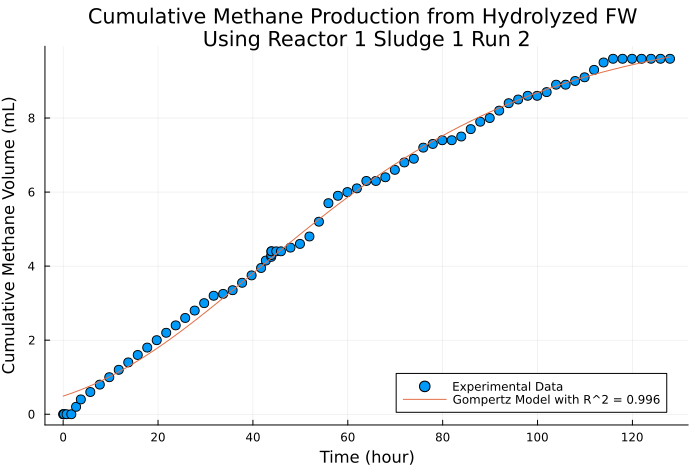
\includegraphics[width=.9\linewidth]{../plots/BMPs/Hydrolyzed FW/methane_kinetics_hydrolysate_1_s1_r2_hour.png}
\end{center}

\subsection{Sample 2}
\label{sec:org539a107}
Το δείγμα το οποίο στην υδρόλυση είχε 2 ml από το μιξ. Με βάση το αρχικό πείραμα υδρόλυσης, αυτό και το 4 ml είχαν το καλύτερο performance και ελάχιστη διαφορά μεταξύ τους (κατά βάση στην συγκέντρωση γαλακτικού οξέος) οπότε θα αναμέναμε εδώ να παρατηρηθεί η καλύτερη μεθανογένεση.

\textbf{hydrolysate\textsubscript{2}\textsubscript{s1}\textsubscript{r2}}
\begin{minted}[breaklines=true,breakanywhere=true]{julia}

### Data Analysis on Hydrolysate with 2 ml ###

<<date_saving_fw_s1_r2>>

inds = 4:69
exp_meth_vol = [0, 0.1, 0.1, 1.3, 0, 0.2, 0.1, 0.4, 0.5, 0.2, 0.1, 0.5, 0, 0.1, 0.2, 0.2, 0.2, 0.1, 0.05, 0.05, 0.05, 0, 0.1, 0.1, 0, 0, 0, 0.1, 0.1, 0.2, 0.05, 0, 0.1, 0.1, 0.1, 0.1, 0.1, 0.1, 0.2, 0.2, 0.2, 0.2, 0.1, 0.05, 0.05, 0, 0.05, 0.1, 0.1, 0, 0.05, 0.1, 0.1, 0.2, 0.2, 0, 0.1, 0.1, 0, 0, 0, 0, 0, 0, 0.05, 0.05]
meth_vol_hydro_2 = cumsum(exp_meth_vol)[end]
exp_name = "hydrolysate_2_s1_r2"
source = "Hydrolyzed FW"
sample = "Sample 2"
sludge = "Sludge 1"
run_num = "Run 2"
input_cod = 0.1

<<bmp_data_processing>>

p0 = [100.0, 15.0, 1.0]
<<bmp_curve_fitting_min>>
model_hydro_2_min = vcat(sample, model_params, r_squared)
<<bmp_data_plotting>>

p0 = [100.0, 1.0, 0.03]
<<bmp_curve_fitting_hour>>
model_hydro_2_hour = vcat(sample, model_params, r_squared)
<<bmp_data_plotting>>
\end{minted}

\subsubsection{Results}
\label{sec:org0dae073}
\begin{center}
\begin{tabular}{lrrrr}
Timestamp & Minutes & Hours & Methane\textsubscript{Volume} & Cumulative\textsubscript{Methane}\textsubscript{Volume}\\[0pt]
\hline
03/04\textsubscript{14}:56 & 0.0 & 0.0 & 0.0 & 0.0\\[0pt]
03/04\textsubscript{15}:29 & 32.2709 & 0.5378 & 0.1 & 0.1\\[0pt]
03/04\textsubscript{16}:29 & 92.2712 & 1.5379 & 0.1 & 0.2\\[0pt]
03/04\textsubscript{17}:29 & 152.2757 & 2.5379 & 1.3 & 1.5\\[0pt]
03/04\textsubscript{18}:29 & 212.2757 & 3.5379 & 0.0 & 1.5\\[0pt]
03/04\textsubscript{20}:29 & 332.2757 & 5.5379 & 0.2 & 1.7\\[0pt]
03/04\textsubscript{22}:29 & 452.2757 & 7.5379 & 0.1 & 1.8\\[0pt]
04/04\textsubscript{00}:29 & 572.2824 & 9.538 & 0.4 & 2.2\\[0pt]
04/04\textsubscript{02}:29 & 692.2824 & 11.538 & 0.5 & 2.7\\[0pt]
04/04\textsubscript{04}:29 & 812.2825 & 13.538 & 0.2 & 2.9\\[0pt]
04/04\textsubscript{06}:29 & 932.2824 & 15.538 & 0.1 & 3.0\\[0pt]
04/04\textsubscript{08}:29 & 1052.2865 & 17.5381 & 0.5 & 3.5\\[0pt]
04/04\textsubscript{10}:29 & 1172.2924 & 19.5382 & 0.0 & 3.5\\[0pt]
04/04\textsubscript{12}:29 & 1292.2929 & 21.5382 & 0.1 & 3.6\\[0pt]
04/04\textsubscript{14}:29 & 1412.293 & 23.5382 & 0.2 & 3.8\\[0pt]
04/04\textsubscript{16}:29 & 1532.2929 & 25.5382 & 0.2 & 4.0\\[0pt]
04/04\textsubscript{18}:29 & 1652.3113 & 27.5385 & 0.2 & 4.2\\[0pt]
04/04\textsubscript{20}:29 & 1772.3141 & 29.5386 & 0.1 & 4.3\\[0pt]
04/04\textsubscript{22}:29 & 1892.3154 & 31.5386 & 0.05 & 4.35\\[0pt]
05/04\textsubscript{00}:29 & 2012.3105 & 33.5385 & 0.05 & 4.4\\[0pt]
05/04\textsubscript{02}:29 & 2132.3114 & 35.5385 & 0.05 & 4.45\\[0pt]
05/04\textsubscript{04}:29 & 2252.3144 & 37.5386 & 0.0 & 4.45\\[0pt]
05/04\textsubscript{06}:29 & 2372.3151 & 39.5386 & 0.1 & 4.55\\[0pt]
05/04\textsubscript{08}:29 & 2492.315 & 41.5386 & 0.1 & 4.65\\[0pt]
05/04\textsubscript{09}:29 & 2552.3147 & 42.5386 & 0.0 & 4.65\\[0pt]
05/04\textsubscript{10}:37 & 2620.5911 & 43.6765 & 0.0 & 4.65\\[0pt]
05/04\textsubscript{10}:38 & 2621.5911 & 43.6932 & 0.0 & 4.65\\[0pt]
05/04\textsubscript{10}:39 & 2622.5911 & 43.7099 & 0.1 & 4.75\\[0pt]
05/04\textsubscript{10}:40 & 2623.568 & 43.7261 & 0.1 & 4.85\\[0pt]
05/04\textsubscript{11}:40 & 2683.7432 & 44.7291 & 0.2 & 5.05\\[0pt]
05/04\textsubscript{12}:40 & 2743.749 & 45.7292 & 0.05 & 5.1\\[0pt]
05/04\textsubscript{14}:40 & 2863.749 & 47.7291 & 0.0 & 5.1\\[0pt]
05/04\textsubscript{16}:40 & 2983.7494 & 49.7292 & 0.1 & 5.2\\[0pt]
05/04\textsubscript{18}:40 & 3103.7554 & 51.7293 & 0.1 & 5.3\\[0pt]
05/04\textsubscript{20}:40 & 3223.7562 & 53.7293 & 0.1 & 5.4\\[0pt]
05/04\textsubscript{22}:40 & 3343.7588 & 55.7293 & 0.1 & 5.5\\[0pt]
06/04\textsubscript{00}:40 & 3463.7624 & 57.7294 & 0.1 & 5.6\\[0pt]
06/04\textsubscript{02}:40 & 3583.7627 & 59.7294 & 0.1 & 5.7\\[0pt]
06/04\textsubscript{04}:40 & 3703.7626 & 61.7294 & 0.2 & 5.9\\[0pt]
06/04\textsubscript{06}:40 & 3823.768 & 63.7295 & 0.2 & 6.1\\[0pt]
06/04\textsubscript{08}:40 & 3943.77 & 65.7295 & 0.2 & 6.3\\[0pt]
06/04\textsubscript{10}:40 & 4063.7699 & 67.7295 & 0.2 & 6.5\\[0pt]
06/04\textsubscript{12}:40 & 4183.7779 & 69.7296 & 0.1 & 6.6\\[0pt]
06/04\textsubscript{14}:40 & 4303.7782 & 71.7296 & 0.05 & 6.65\\[0pt]
06/04\textsubscript{16}:40 & 4423.7808 & 73.7297 & 0.05 & 6.7\\[0pt]
06/04\textsubscript{18}:40 & 4543.7815 & 75.7297 & 0.0 & 6.7\\[0pt]
06/04\textsubscript{20}:40 & 4663.7816 & 77.7297 & 0.05 & 6.75\\[0pt]
06/04\textsubscript{22}:40 & 4783.7816 & 79.7297 & 0.1 & 6.85\\[0pt]
07/04\textsubscript{00}:40 & 4903.7918 & 81.7299 & 0.1 & 6.95\\[0pt]
07/04\textsubscript{02}:40 & 5023.7924 & 83.7299 & 0.0 & 6.95\\[0pt]
07/04\textsubscript{04}:40 & 5143.7925 & 85.7299 & 0.05 & 7.0\\[0pt]
07/04\textsubscript{06}:40 & 5263.7924 & 87.7299 & 0.1 & 7.1\\[0pt]
07/04\textsubscript{08}:40 & 5383.7944 & 89.7299 & 0.1 & 7.2\\[0pt]
07/04\textsubscript{10}:40 & 5503.8038 & 91.7301 & 0.2 & 7.4\\[0pt]
07/04\textsubscript{12}:40 & 5623.8058 & 93.7301 & 0.2 & 7.6\\[0pt]
07/04\textsubscript{14}:40 & 5743.8073 & 95.7301 & 0.0 & 7.6\\[0pt]
07/04\textsubscript{16}:40 & 5863.8086 & 97.7301 & 0.1 & 7.7\\[0pt]
07/04\textsubscript{18}:40 & 5983.8149 & 99.7302 & 0.1 & 7.8\\[0pt]
07/04\textsubscript{20}:40 & 6103.8161 & 101.7303 & 0.0 & 7.8\\[0pt]
07/04\textsubscript{22}:40 & 6223.8172 & 103.7303 & 0.0 & 7.8\\[0pt]
08/04\textsubscript{00}:40 & 6343.8343 & 105.7306 & 0.0 & 7.8\\[0pt]
08/04\textsubscript{02}:40 & 6463.8355 & 107.7306 & 0.0 & 7.8\\[0pt]
08/04\textsubscript{04}:40 & 6583.8267 & 109.7304 & 0.0 & 7.8\\[0pt]
08/04\textsubscript{06}:40 & 6703.826 & 111.7304 & 0.0 & 7.8\\[0pt]
08/04\textsubscript{08}:40 & 6823.8259 & 113.7304 & 0.05 & 7.85\\[0pt]
08/04\textsubscript{10}:40 & 6943.8258 & 115.7304 & 0.05 & 7.9\\[0pt]
\end{tabular}
\end{center}


\begin{center}
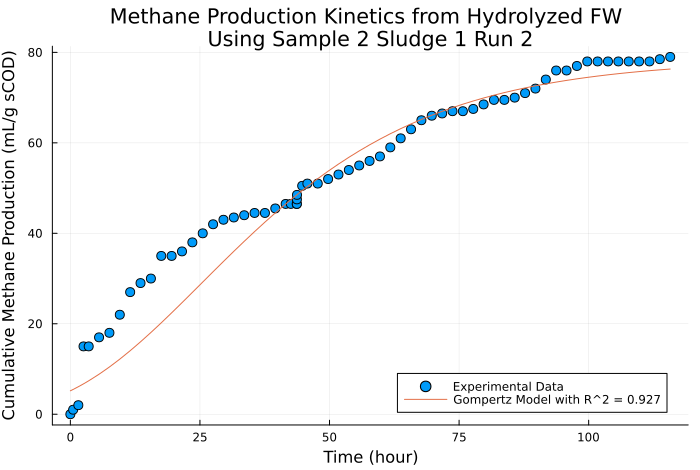
\includegraphics[width=.9\linewidth]{../plots/BMPs/Hydrolyzed FW/methane_kinetics_hydrolysate_2_s1_r2_hour.png}
\end{center}

\subsection{Sample 4}
\label{sec:org690957a}
Το δείγμα 4 ήταν αυτό με τα 4 ml mix στην υδρόλυση. Είναι η μέγιστη ποσότητα που χρησιμοποιήθηκε για τα πειράματα χώνευσης καθώς το 8 ml δεν είχε ιδιαίτερα μεγάλη διαφορά και είναι πολύ πιο ακριβό. Όπως προαναφέρθηκε, αναμένουμε να έχει παρόμοια ποιότητα με το 2 ml καθώς με εξαίρεση μίας ποσότητας γαλακτικού είναι σχεδόν ίδια.

\textbf{hydrolysate\textsubscript{4}\textsubscript{s1}\textsubscript{r2}}
\begin{minted}[breaklines=true,breakanywhere=true]{julia}

### Data Analysis on Hydrolysate with 4 ml ###

<<date_saving_fw_s1_r2>>

inds = 3:69
exp_meth_vol = [0, 0, 0, 0, 0.05, 0.1, 0.1, 0.3, 0.3, 0.3, 0.3, 0.3, 0.1, 0.2, 0.1, 0.1, 0.2, 0.1, 0.1, 0.05, 0.1, 0.2, 0.2, 0.1, 0.05, 0.1, 0.1, 0, 0, 0, 0, 0.1, 0.1, 0.2, 0.1, 0.1, 0.1, 0.1, 0.1, 0.1, 0.2, 0.1, 0.1, 0.2, 0.1, 0.2, 0.1, 0.1, 0.1, 0.1, 0.1, 0.2, 0.1, 0.1, 0.1, 0.1, 0.1, 0.2, 0.2, 0.1, 0, 0, 0.05, 0.05, 0, 0.05, 0.1]
meth_vol_hydro_4 = cumsum(exp_meth_vol)[end]
exp_name = "hydrolysate_4_s1_r2"
source = "Hydrolyzed FW"
sample = "Sample 4"
sludge = "Sludge 1"
run_num = "Run 2"

input_cod = 0.1

<<bmp_data_processing>>

p0 = [170.0, 150.0, 1.0]
<<bmp_curve_fitting_min>>
model_hydro_4_min = vcat(sample, model_params, r_squared)
<<bmp_data_plotting>>

p0 = [170.0, 1000.0, 0.1]
<<bmp_curve_fitting_hour>>
model_hydro_4_hour = vcat(sample, model_params, r_squared)
<<bmp_data_plotting>>
\end{minted}

\subsubsection{Results}
\label{sec:orgc090943}

\begin{center}
\begin{tabular}{lrrrr}
Timestamp & Minutes & Hours & Methane\textsubscript{Volume} & Cumulative\textsubscript{Methane}\textsubscript{Volume}\\[0pt]
\hline
03/04\textsubscript{14}:51 & 0.0 & 0.0 & 0.0 & 0.0\\[0pt]
03/04\textsubscript{14}:56 & 5.0455 & 0.0841 & 0.0 & 0.0\\[0pt]
03/04\textsubscript{15}:29 & 37.3164 & 0.6219 & 0.0 & 0.0\\[0pt]
03/04\textsubscript{16}:29 & 97.3168 & 1.6219 & 0.0 & 0.0\\[0pt]
03/04\textsubscript{17}:29 & 157.3212 & 2.622 & 0.05 & 0.05\\[0pt]
03/04\textsubscript{18}:29 & 217.3212 & 3.622 & 0.1 & 0.15\\[0pt]
03/04\textsubscript{20}:29 & 337.3212 & 5.622 & 0.1 & 0.25\\[0pt]
03/04\textsubscript{22}:29 & 457.3212 & 7.622 & 0.3 & 0.55\\[0pt]
04/04\textsubscript{00}:29 & 577.3279 & 9.6221 & 0.3 & 0.85\\[0pt]
04/04\textsubscript{02}:29 & 697.3279 & 11.6221 & 0.3 & 1.15\\[0pt]
04/04\textsubscript{04}:29 & 817.328 & 13.6221 & 0.3 & 1.45\\[0pt]
04/04\textsubscript{06}:29 & 937.3279 & 15.6221 & 0.3 & 1.75\\[0pt]
04/04\textsubscript{08}:29 & 1057.332 & 17.6222 & 0.1 & 1.85\\[0pt]
04/04\textsubscript{10}:29 & 1177.3379 & 19.6223 & 0.2 & 2.05\\[0pt]
04/04\textsubscript{12}:29 & 1297.3384 & 21.6223 & 0.1 & 2.15\\[0pt]
04/04\textsubscript{14}:29 & 1417.3385 & 23.6223 & 0.1 & 2.25\\[0pt]
04/04\textsubscript{16}:29 & 1537.3384 & 25.6223 & 0.2 & 2.45\\[0pt]
04/04\textsubscript{18}:29 & 1657.3568 & 27.6226 & 0.1 & 2.55\\[0pt]
04/04\textsubscript{20}:29 & 1777.3596 & 29.6227 & 0.1 & 2.65\\[0pt]
04/04\textsubscript{22}:29 & 1897.3609 & 31.6227 & 0.05 & 2.7\\[0pt]
05/04\textsubscript{00}:29 & 2017.356 & 33.6226 & 0.1 & 2.8\\[0pt]
05/04\textsubscript{02}:29 & 2137.3569 & 35.6226 & 0.2 & 3.0\\[0pt]
05/04\textsubscript{04}:29 & 2257.3599 & 37.6227 & 0.2 & 3.2\\[0pt]
05/04\textsubscript{06}:29 & 2377.3606 & 39.6227 & 0.1 & 3.3\\[0pt]
05/04\textsubscript{08}:29 & 2497.3605 & 41.6227 & 0.05 & 3.35\\[0pt]
05/04\textsubscript{09}:29 & 2557.3602 & 42.6227 & 0.1 & 3.45\\[0pt]
05/04\textsubscript{10}:37 & 2625.6366 & 43.7606 & 0.1 & 3.55\\[0pt]
05/04\textsubscript{10}:38 & 2626.6366 & 43.7773 & 0.0 & 3.55\\[0pt]
05/04\textsubscript{10}:39 & 2627.6366 & 43.7939 & 0.0 & 3.55\\[0pt]
05/04\textsubscript{10}:40 & 2628.6134 & 43.8102 & 0.0 & 3.55\\[0pt]
05/04\textsubscript{11}:40 & 2688.7887 & 44.8131 & 0.0 & 3.55\\[0pt]
05/04\textsubscript{12}:40 & 2748.7945 & 45.8132 & 0.1 & 3.65\\[0pt]
05/04\textsubscript{14}:40 & 2868.7944 & 47.8132 & 0.1 & 3.75\\[0pt]
05/04\textsubscript{16}:40 & 2988.7949 & 49.8132 & 0.2 & 3.95\\[0pt]
05/04\textsubscript{18}:40 & 3108.8008 & 51.8133 & 0.1 & 4.05\\[0pt]
05/04\textsubscript{20}:40 & 3228.8017 & 53.8134 & 0.1 & 4.15\\[0pt]
05/04\textsubscript{22}:40 & 3348.8043 & 55.8134 & 0.1 & 4.25\\[0pt]
06/04\textsubscript{00}:40 & 3468.808 & 57.8135 & 0.1 & 4.35\\[0pt]
06/04\textsubscript{02}:40 & 3588.8082 & 59.8135 & 0.1 & 4.45\\[0pt]
06/04\textsubscript{04}:40 & 3708.8081 & 61.8135 & 0.1 & 4.55\\[0pt]
06/04\textsubscript{06}:40 & 3828.8134 & 63.8136 & 0.2 & 4.75\\[0pt]
06/04\textsubscript{08}:40 & 3948.8154 & 65.8136 & 0.1 & 4.85\\[0pt]
06/04\textsubscript{10}:40 & 4068.8154 & 67.8136 & 0.1 & 4.95\\[0pt]
06/04\textsubscript{12}:40 & 4188.8234 & 69.8137 & 0.2 & 5.15\\[0pt]
06/04\textsubscript{14}:40 & 4308.8236 & 71.8137 & 0.1 & 5.25\\[0pt]
06/04\textsubscript{16}:40 & 4428.8263 & 73.8138 & 0.2 & 5.45\\[0pt]
06/04\textsubscript{18}:40 & 4548.827 & 75.8138 & 0.1 & 5.55\\[0pt]
06/04\textsubscript{20}:40 & 4668.8271 & 77.8138 & 0.1 & 5.65\\[0pt]
06/04\textsubscript{22}:40 & 4788.8271 & 79.8138 & 0.1 & 5.75\\[0pt]
07/04\textsubscript{00}:40 & 4908.8373 & 81.814 & 0.1 & 5.85\\[0pt]
07/04\textsubscript{02}:40 & 5028.8379 & 83.814 & 0.1 & 5.95\\[0pt]
07/04\textsubscript{04}:40 & 5148.838 & 85.814 & 0.2 & 6.15\\[0pt]
07/04\textsubscript{06}:40 & 5268.8379 & 87.814 & 0.1 & 6.25\\[0pt]
07/04\textsubscript{08}:40 & 5388.8399 & 89.814 & 0.1 & 6.35\\[0pt]
07/04\textsubscript{10}:40 & 5508.8493 & 91.8142 & 0.1 & 6.45\\[0pt]
07/04\textsubscript{12}:40 & 5628.8513 & 93.8142 & 0.1 & 6.55\\[0pt]
07/04\textsubscript{14}:40 & 5748.8528 & 95.8142 & 0.1 & 6.65\\[0pt]
07/04\textsubscript{16}:40 & 5868.8541 & 97.8142 & 0.2 & 6.85\\[0pt]
07/04\textsubscript{18}:40 & 5988.8604 & 99.8143 & 0.2 & 7.05\\[0pt]
07/04\textsubscript{20}:40 & 6108.8616 & 101.8144 & 0.1 & 7.15\\[0pt]
07/04\textsubscript{22}:40 & 6228.8628 & 103.8144 & 0.0 & 7.15\\[0pt]
08/04\textsubscript{00}:40 & 6348.8798 & 105.8147 & 0.0 & 7.15\\[0pt]
08/04\textsubscript{02}:40 & 6468.881 & 107.8147 & 0.05 & 7.2\\[0pt]
08/04\textsubscript{04}:40 & 6588.8722 & 109.8145 & 0.05 & 7.25\\[0pt]
08/04\textsubscript{06}:40 & 6708.8714 & 111.8145 & 0.0 & 7.25\\[0pt]
08/04\textsubscript{08}:40 & 6828.8714 & 113.8145 & 0.05 & 7.3\\[0pt]
08/04\textsubscript{10}:40 & 6948.8713 & 115.8145 & 0.1 & 7.4\\[0pt]
\end{tabular}
\end{center}


\begin{center}
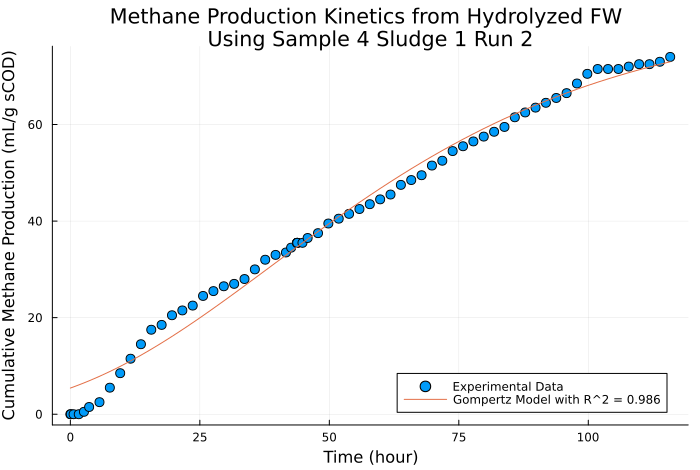
\includegraphics[width=.9\linewidth]{../plots/BMPs/Hydrolyzed FW/methane_kinetics_hydrolysate_4_s1_r2_hour.png}
\end{center}

\subsection{Untreated FW}
\label{sec:org497eacc}
Εκτός από τα παραπάνω, σε ένα από τα δοχεία προστέθηκε ανεπεξέργαστο FW. Αυτό έχει διαφορά από το δείγμα 0, καθώς εκείνο υπέστει ζύμωση κατά τις 72 ώρες που ήταν στους 40 \(^oC\) ακόμη και χωρίς να προσθέσουμε κάποιο εμβόλιο, ενώ το δείγμα αυτό αναφέρεται σε food waste το οποίο δεν έχει υποστεί καμία επεξεργασία. Θα θέλαμε το δείγμα αυτό να έχει το χειρότερο performance (είτε πολύ αργή παραγωγή, ή μικρή τελική παραγωγή), το οποίο θα μας επιδείκνυε πως η επεξεργασία που έγινε βοηθάει πραγματικά στην χώνευση. Βέβαια, αξίζει να αναφερθεί πως το δοχείο αυτό είχε κάποιο προβλήματα με διαρροή στα αρχικά στάδια του πειράματος, οπότε ενδέχεται τα αποτελέσματα που θα προκύψουν να μην είναι έγκυρα. Παρακάτω φαίνεται ο κώδικας επεξεργασίας των αποτελεσμάτων του.

\textbf{untreated\textsubscript{fw}\textsubscript{s1}\textsubscript{r2}}
\begin{minted}[breaklines=true,breakanywhere=true]{julia}

### Data Analysis on Untreated FW ###

<<date_saving_fw_s1_r2>>

inds = 29:62
exp_meth_vol = [0, 0, 5, 1, 0, 0.1, 0.2, 0.2, 0.1, 0.1, 0.1, 0.1, 0.1, 0.05, 0.05, 0, 0, 0.2, 0.2, 0.1, 0.1, 0.1, 0, 0.1, 0.1, 0.1, 0.1, 0, 0.1, 0.05, 0, 0, 0, 0]
meth_vol_hydro_fw = cumsum(exp_meth_vol)[end]
exp_name = "untreated_fw_s1_r2"
source = "Untreated FW"
sample = ""
sludge = "Sludge 1"
run_num = "Run 2"

input_cod = 0.1

<<bmp_data_processing>>

p0 = [75.0, 100.0, 1.0]
<<bmp_curve_fitting_min>>
model_hydro_fw_min = vcat(sample, model_params, r_squared)
<<bmp_data_plotting>>

p0 = [75.0, 1.0, 0.1]
<<bmp_curve_fitting_hour>>
model_hydro_fw_hour = vcat(sample, model_params, r_squared)
<<bmp_data_plotting>>
\end{minted}

\subsubsection{Results}
\label{sec:org22be743}

\begin{center}
\begin{tabular}{lrrrr}
Timestamp & Minutes & Hours & Methane\textsubscript{Volume} & Cumulative\textsubscript{Methane}\textsubscript{Volume}\\[0pt]
\hline
05/04\textsubscript{10}:37 & 0.0 & 0.0 & 0.0 & 0.0\\[0pt]
05/04\textsubscript{10}:38 & 1.0 & 0.0167 & 0.0 & 0.0\\[0pt]
05/04\textsubscript{10}:39 & 1.9999 & 0.0333 & 5.0 & 5.0\\[0pt]
05/04\textsubscript{10}:40 & 2.9768 & 0.0496 & 1.0 & 6.0\\[0pt]
05/04\textsubscript{11}:40 & 63.1521 & 1.0525 & 0.0 & 6.0\\[0pt]
05/04\textsubscript{12}:40 & 123.1579 & 2.0526 & 0.1 & 6.1\\[0pt]
05/04\textsubscript{14}:40 & 243.1578 & 4.0526 & 0.2 & 6.3\\[0pt]
05/04\textsubscript{16}:40 & 363.1583 & 6.0526 & 0.2 & 6.5\\[0pt]
05/04\textsubscript{18}:40 & 483.1642 & 8.0527 & 0.1 & 6.6\\[0pt]
05/04\textsubscript{20}:40 & 603.1651 & 10.0528 & 0.1 & 6.7\\[0pt]
05/04\textsubscript{22}:40 & 723.1677 & 12.0528 & 0.1 & 6.8\\[0pt]
06/04\textsubscript{00}:40 & 843.1713 & 14.0529 & 0.1 & 6.9\\[0pt]
06/04\textsubscript{02}:40 & 963.1716 & 16.0529 & 0.1 & 7.0\\[0pt]
06/04\textsubscript{04}:40 & 1083.1714 & 18.0529 & 0.05 & 7.05\\[0pt]
06/04\textsubscript{06}:40 & 1203.1768 & 20.0529 & 0.05 & 7.1\\[0pt]
06/04\textsubscript{08}:40 & 1323.1788 & 22.053 & 0.0 & 7.1\\[0pt]
06/04\textsubscript{10}:40 & 1443.1788 & 24.053 & 0.0 & 7.1\\[0pt]
06/04\textsubscript{12}:40 & 1563.1868 & 26.0531 & 0.2 & 7.3\\[0pt]
06/04\textsubscript{14}:40 & 1683.187 & 28.0531 & 0.2 & 7.5\\[0pt]
06/04\textsubscript{16}:40 & 1803.1897 & 30.0532 & 0.1 & 7.6\\[0pt]
06/04\textsubscript{18}:40 & 1923.1903 & 32.0532 & 0.1 & 7.7\\[0pt]
06/04\textsubscript{20}:40 & 2043.1904 & 34.0532 & 0.1 & 7.8\\[0pt]
06/04\textsubscript{22}:40 & 2163.1905 & 36.0532 & 0.0 & 7.8\\[0pt]
07/04\textsubscript{00}:40 & 2283.2007 & 38.0533 & 0.1 & 7.9\\[0pt]
07/04\textsubscript{02}:40 & 2403.2013 & 40.0534 & 0.1 & 8.0\\[0pt]
07/04\textsubscript{04}:40 & 2523.2014 & 42.0534 & 0.1 & 8.1\\[0pt]
07/04\textsubscript{06}:40 & 2643.2013 & 44.0534 & 0.1 & 8.2\\[0pt]
07/04\textsubscript{08}:40 & 2763.2033 & 46.0534 & 0.0 & 8.2\\[0pt]
07/04\textsubscript{10}:40 & 2883.2126 & 48.0535 & 0.1 & 8.3\\[0pt]
07/04\textsubscript{12}:40 & 3003.2147 & 50.0536 & 0.05 & 8.35\\[0pt]
07/04\textsubscript{14}:40 & 3123.2162 & 52.0536 & 0.0 & 8.35\\[0pt]
07/04\textsubscript{16}:40 & 3243.2175 & 54.0536 & 0.0 & 8.35\\[0pt]
07/04\textsubscript{18}:40 & 3363.2237 & 56.0537 & 0.0 & 8.35\\[0pt]
07/04\textsubscript{20}:40 & 3483.225 & 58.0538 & 0.0 & 8.35\\[0pt]
\end{tabular}
\end{center}


\begin{center}
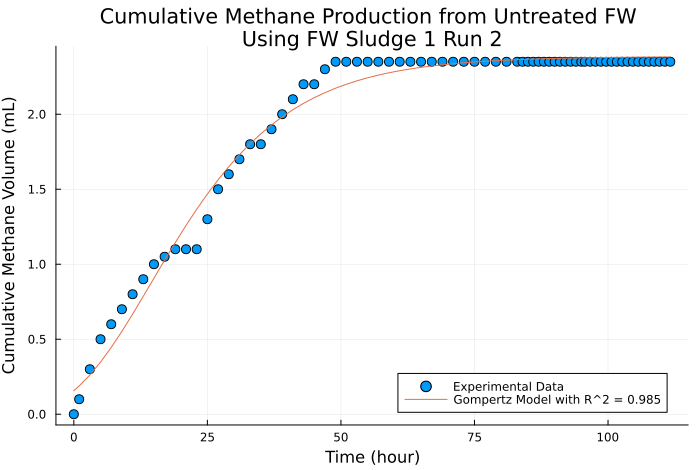
\includegraphics[width=.9\linewidth]{../plots/BMPs/Untreated FW/methane_kinetics_untreated_fw_s1_r2_hour.png}
\end{center}

\subsection{Untreated FW Correction}
\label{sec:org0d17f56}
Στο δείγμα αυτό, το σημείο 3 το οποίο είναι 5 ml ενδέχεται να μην είναι αέριο που παράγεται αλλά να έχει προκληθεί από διαφορά πίεσης μόλις προστέθηκε δείγμα. Η ύπαρξη του είναι γενικά προβληματική, οπότε θέλουμε να δούμε τι γίνεται αν αυτό αγνοηθεί.

\textbf{untreated\textsubscript{fw}\textsubscript{s1}\textsubscript{r2}\textsubscript{corr}}
\begin{minted}[breaklines=true,breakanywhere=true]{julia}

### Data Analysis on Untreated FW ###

<<date_saving_fw_s1_r2>>

inds = 33:62
exp_meth_vol = [0, 0.1, 0.2, 0.2, 0.1, 0.1, 0.1, 0.1, 0.1, 0.05, 0.05, 0, 0, 0.2, 0.2, 0.1, 0.1, 0.1, 0, 0.1, 0.1, 0.1, 0.1, 0, 0.1, 0.05, 0, 0, 0, 0]
meth_vol_hydro_fw_corr = cumsum(exp_meth_vol)[end]
exp_name = "untreated_fw_s1_r2_corr"
source = "Untreated FW"
sample = ""
sludge = "Sludge 1"
run_num = "Run 2"

input_cod = 0.1

<<bmp_data_processing>>

p0 = [75.0, 1.0, 1.0]
<<bmp_curve_fitting_min>>
model_hydro_fw_corr_min = vcat(sample, model_params, r_squared)
<<bmp_data_plotting>>

p0 = [75.0, 1.2, 0.1]
<<bmp_curve_fitting_hour>>
model_hydro_fw_corr_hour = vcat(sample, model_params, r_squared)
<<bmp_data_plotting>>
\end{minted}

\begin{center}
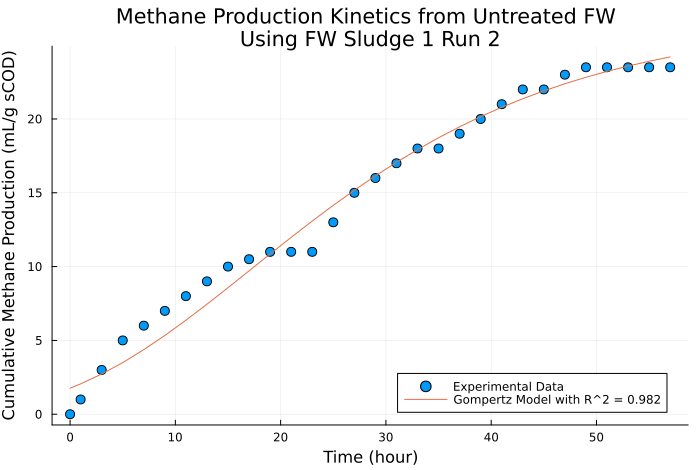
\includegraphics[width=.9\linewidth]{../plots/BMPs/Untreated FW/methane_kinetics_untreated_fw_s1_r2_corr_hour.png}
\end{center}

Αφαιρώντας την περίεργη αυτή αρχή του πειράματος, για την οποία μπορεί να μην ευθύνεται το μεθάνιο, βλέπουμε πως η καμπύλη έχει μία τέλεια προσαρμογή στα πειραματικά δεδομένα με R\textsuperscript{2} = 0.982.

\subsection{Update all}
\label{sec:orga64507c}
Όπως και για τα προηγούμενα, θα υπάρχει και ένα code block το οποίο θα κάνει update όλα τα code blocks, θα τα κάνει tangle σε ένα script file και θα αποθηκεύει ένα CSV με όλα τα κινητικά αποτελέσματα.

\textbf{update\textsubscript{hydrolysate}\textsubscript{tests}\textsubscript{s1}\textsubscript{r2}}
\begin{minted}[breaklines=true,breakanywhere=true]{julia}

<<hydrolysate_0_s1_r2>>
<<hydrolysate_1_s1_r2>>
<<hydrolysate_2_s1_r2>>
<<hydrolysate_4_s1_r2>>
<<untreated_fw_s1_r2>>
<<untreated_fw_s1_r2_corr>>

model_fit_table_min = Tables.table(vcat(reshape(model_hydro_0_min, 1, 5), reshape(model_hydro_1_min, 1, 5), reshape(model_hydro_2_min, 1, 5), reshape(model_hydro_4_min, 1, 5), reshape(model_hydro_fw_min, 1, 5), reshape(model_hydro_fw_corr_min, 1, 5)), header = [:Sample_Name, :Methane_Production_Potential, :Methane_Production_Rate, :Lag_Time, :R_squared])
CSV.write(datadir("exp_pro", "methane_from_hydrolysate_kinetics_min_s1_r2.csv"), model_fit_table_min)

model_fit_table_hour = Tables.table(vcat(reshape(model_hydro_0_hour, 1, 5), reshape(model_hydro_1_hour, 1, 5), reshape(model_hydro_2_hour, 1, 5), reshape(model_hydro_4_hour, 1, 5), reshape(model_hydro_fw_hour, 1, 5), reshape(model_hydro_fw_corr_hour, 1, 5)), header = [:Sample_Name, :Methane_Production_Potential, :Methane_Production_Rate, :Lag_Time, :R_squared])
CSV.write(datadir("exp_pro", "methane_from_hydrolysate_kinetics_hour_s1_r2.csv"), model_fit_table_hour)
\end{minted}

\begin{table}[htbp]
\caption{Kinetics with timescale in hours}
\centering
\begin{tabular}{lrrrr}
Sample\textsubscript{Name} & Production\textsubscript{Potential} & Production\textsubscript{Rate} & Lag\textsubscript{Time} & R\textsubscript{squared}\\[0pt]
\hline
Sample 0 & 37.583 & 0.434 & 3.763 & 0.991\\[0pt]
Sample 1 & 104.279 & 1.075 & 4.507 & 0.995\\[0pt]
Sample 2 & 78.458 & 1.144 & 0.0 & 0.927\\[0pt]
Sample 4 & 83.674 & 0.796 & 0.265 & 0.986\\[0pt]
FW & 767.403 & 1.167 & 0.0 & 0.464\\[0pt]
FW\textsubscript{corrected} & 26.719 & 0.571 & 0.0 & 0.982\\[0pt]
\end{tabular}
\end{table}

\begin{table}[htbp]
\caption{Kinetics with timescale in minutes}
\centering
\begin{tabular}{lrrrr}
Sample\textsubscript{Name} & Production\textsubscript{Potential} & Production\textsubscript{Rate} & Lag\textsubscript{Time} & R\textsubscript{squared}\\[0pt]
\hline
Sample 0 & 37.583 & 0.00722 & 225.800 & 0.991\\[0pt]
Sample 1 & 104.279 & 0.0179 & 270.399 & 0.995\\[0pt]
Sample 2 & 76.957 & 0.0205 & 0.0 & 0.933\\[0pt]
Sample 4 & 83.675 & 0.0132 & 15.910 & 0.986\\[0pt]
FW & 74.291 & 49.128 & 1.041 & 0.863\\[0pt]
FW\textsubscript{corrected} & 26.910 & 0.00938 & 0.0 & 0.982\\[0pt]
\end{tabular}
\end{table}

\subsection{Plotting Methane Potential}
\label{sec:orgf537cf2}
Σε αυτό το section θα γίνει ένα plot το οποίο θα συγκρίνει μέγιστο μεθάνιο (παραγωγή από οξικό) με αυτό που παράχθηκε από το FW. Το plotting θα γίνει μέσω του \texttt{CairoMakie.jl} το οποίο είναι αρκετά featureful. Αρχικά όμως πρέπει να κάνουμε κάποιο data collection για να γίνει το plotting. Τρέχουμε τα 2 code blocks που κάνουν update όλα τα πειράματα με βασικό σκοπό να αποθηκεύσουμε τον τελικό όγκο σε κάθε πείραμα. Έπειτα βάζουμε όλα αυτά σε ένα vector και εκτός από την απόλυτη τιμή, υπολογίζουμε και το ποσοστό του μέγιστου που πετυχαίνει το υδρόλυμα. Όπως έχουν αποθηκευτεί, αυτό είναι διαίρεση του στοιχείου i+5 με το i. Έπειτα φτιάχνουμε ένα string των ποσοστών αυτών μαζί με τα labels που τους αντιστοιχούν. Αυτό θα προστεθεί στο plot που φτιάχνουμε.

\begin{minted}[breaklines=true,breakanywhere=true]{julia}

<<update_acetate_tests_s1>>
<<update_hydrolysate_tests_s1_r2>>

comp_name = "s1_r2"
\end{minted}

Έχοντας κάνει το preprocessing αυτό, ξεκινάμε την δημιουργία διαγραμμάτων. Φτιάχνουμε ένα figure και έναν άξονα πάνω σε αυτό όπου θα κάνουμε τα bar plots που θέλουμε. Οι μεταβλητές \texttt{xdata} και \texttt{grp} είναι απαραίτητες για να φτιαχτεί το plot. Το xdata λέει σε ποιό σημείο του άξονα x θα πάει κάθε δεδομένο (όπως τα έχουμε ορίσει θα είναι από το 1 εώς το 5 δύο φορές) ενώ το grp λέει σε ποιό group θα ανήκει το κάθε πείραμα. Τα 5 πρώτα είναι στο group 1 (οξικό) ενώ τα άλλα στο 2 (υδρόλυμα). Ορίζουμε και το legend και το plot αυτό είναι έτοιμο. Από κάτω, κάνουμε insert το string με τα ποσοστά που υπολογίστηκε παραπάνω σε ένα text plot του Makie. Έπειτα, κάνουμε save το plot αυτό.

\begin{minted}[breaklines=true,breakanywhere=true]{julia}

using CairoMakie
colors = Makie.wong_colors()

meth_vol = [meth_vol_acet_0, meth_vol_acet_1, meth_vol_acet_2, meth_vol_acet_4, meth_vol_acet_fw, meth_vol_hydro_0, meth_vol_hydro_1, meth_vol_hydro_2, meth_vol_hydro_4, meth_vol_hydro_fw, meth_vol_hydro_fw_corr]

percent_bmp = vcat([meth_vol[i+5]/meth_vol[i] for i in 1:5], meth_vol[11]/meth_vol[5])
string_bmp = vcat(string.(round.(percent_bmp.*100, digits = 2)).*" %", ["0 ml", "1 ml", "2 ml", "4 ml", "Untreated \nFW", "Untreated FW \nCorrected"])

fig = Figure(size = (600, 400))
ax = Axis(fig[1,1], xticks = (1:5, ["0 ml", "1 ml", "2 ml", "4 ml", "Untreated FW"]),
          title = "Acetate vs Hydrolysate BMP")

xdata = [1, 2, 3, 4, 5, 1, 2, 3, 4, 5, 5]
grp = [1, 1, 1, 1, 1, 2, 2, 2, 2, 2, 3]

barplot!(ax, xdata, meth_vol,
        dodge = grp,
        color = colors[grp])

# Legend
labels = ["Acetate", "FW", "FW Corrected"]
elements = [PolyElement(polycolor = colors[i]) for i in 1:length(labels)]
title = "Source"
Legend(fig[1,2], elements, labels, title)

xdata_2 = [1, 2, 3, 4, 5, 6, 1, 2, 3, 4, 5, 6]
ax2 = Axis(fig[2, 1:2], xticks = (1:6, ["0 ml", "1 ml", "2 ml", "4 ml", "Untreated FW", "Untreated FW Corrected"]), yticks = ([1, 2], ["", ""]), title = "% of Acetate BMP in Hydrolysates")
hidespines!(ax2)
hidedecorations!(ax2)
text!(xdata_2, repeat(1:1, 12), text = string_bmp, align = [(:left, :top), (:left, :top), (:center, :top), (:center, :top), (:right, :top), (:right, :top), (:left, :bottom), (:left, :bottom), (:center, :bottom), (:center, :bottom), (:right, :bottom), (:right, :bottom)])

save(plotsdir("BMPs", "Hydrolyzed FW", "acet_vs_hydro_bmp_"*comp_name*".png"), fig)
\end{minted}

\begin{center}
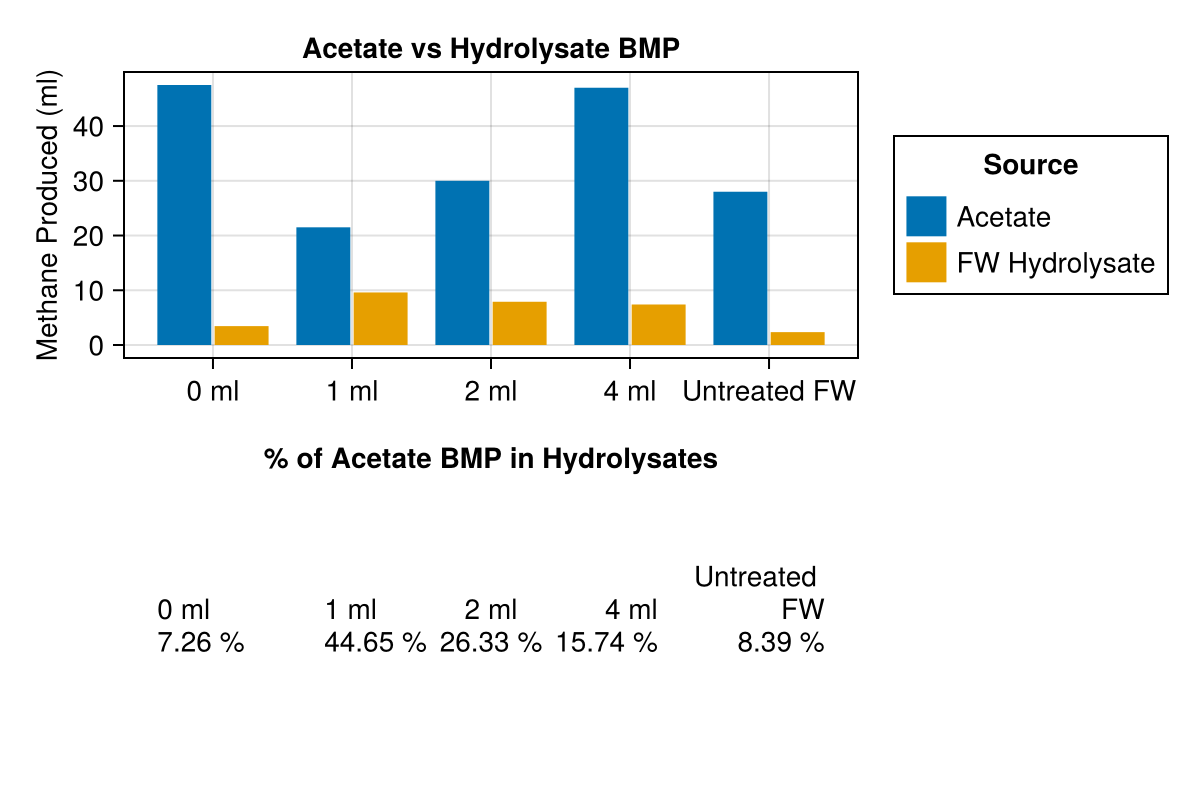
\includegraphics[width=.9\linewidth]{../plots/BMPs/Hydrolyzed FW/acet_vs_hydro_bmp_s1_r2.png}
\end{center}

\subsection{Συμπεράσματα από τον κύκλο πειραμάτων αυτών}
\label{sec:orgc9bcd79}
Το πιο εύκολο συμπέρασμα που βγαίνει από τον κύκλο αυτόν είναι πως τα "περίεργα" αποτελέσματα του πρώτου κύκλου δεν είναι επαναλήψιμα. Με εξαίρεση το δείγμα του ανεπεξέργαστου FW, τα άλλα 4 είχαν έναν σχετικά αργό ρυθμό, ο οποίος ήταν της ίδιας τάξης με τον "αργό" ρυθμό του προηγούμενου πειράματος. Η παραγωγή μεθανίου είναι χαμηλότερη από αυτή του προηγούμενου πειράματος. Τα πειράματα αυτά είχαν επίσης lag time, το οποίο ήταν παραπάνω από μερικά λεπτά (με εξαίρεση του 2 ml, το οποίο δεν φάνηκε να έχει αυτό το πρόβλημα). Ακόμη, τα αποτελέσματα αυτά οδηγούν σε μοντέλα με πάρα πολύ καλό συντελεστή R\textsuperscript{2} (από 0.93 εώς και 0.99).

Όλα αυτά οδηγούν στην υπόθεση ότι αυτό το πείραμα έχει τα "σωστά" αποτελέσματα και η αρχή των προηγούμενων πειραμάτων είχε κάποιο πρόβλημα. Μία πιθανή εξήγηση που μπορεί να δωθεί για τους πολύ γρήγορους ρυθμούς και παραγωγή μεγάλης ποσότητας μεθανίου με μηδενικό lag time είναι ότι εφόσον το πείραμα αυτό έγινε αμέσως μετά το οξικό, οι μικροοργανισμοί είχαν κρατήσει κάποια ποσότητα οξικού και την μεταβόλισαν μόλις δημιουργήθηκε ερέθισμα (προσθήκη νέου υποστρώματος), το οποίο οδήγησε σε πολύ γρήγορο ρυθμό στην αρχή και πολύ μεγάλη επιβράδυνση μετά από μερικές ώρες όταν καταναλώθηκε η ποσότητα οξικού που υπήρχε. Ως αποτέλεσμα, είχε πολύ χειρότερη προσαρμογή, το φαινόμενο των 2 ρυθμών και τις άλλες ιδιορυθμίες που δεν υπήρξαν στην επανάληψη.

Βέβαια, αξίζει να αναφερθεί πως τα ίδια ακριβώς φαινόμενα παρατηρήθηκαν σε αυτό το πείραμα στο ακατέργαστο FW. Λύθηκε το πρόβλημα της διαρροής του δοχείου και είχε μία σημαντική παραγωγή μεθανίου, αλλά αυτή ακολούθησε εκείνες τις ιδιορυθμίες, με συμπέρασμα ότι μάλλον δεν υπάρχει κάποιο πείραμα με ακατέργαστο FW το οποίο να έχει ιδιαίτερα έγκυρα αποτελέσματα.

Από την άποψη των BMPs, χωρίς το untreated FW (το οποίο ενδέχεται να έχει παραπάνω παραγωγή από ότι πρέπει λόγω των παραπάνω παρατηρήσεων), η σειρά είναι 0 > 4 > 2 > 1. Το 0 είναι πάλι το χαμηλότερο, το οποίο κάνει ξανά validate ότι η προσθήκη του μιξ βοηθάει στην προεπεξεργασία και κάνει το υδρόλυμα πιο αποτελεσματικό για την παραγωγή μεθανίου. Το δείγμα 1 έχει και πάλι την περισσότερη ποσότητα μεθανίου. Αυτό δεν μπορεί να αιτιολογηθεί από τα αποτελέσματα του αρχικού πειράματος υδρόλυσης σε αυτές τις συνθήκες, αλλά η αναπάντεχα μεγάλη συγκέντρωση sCOD του, οδηγεί στο συμπέρασμα της καλύτερης διαλυτοποίησης σε αυτό το πείραμα και πιθανόν αυτό να ευθύνεται για την αυξημένη παραγωγή μεθανίου.

\section{Πίνακας με κινητικά δεδομένα}
\label{sec:orgbc641cc}
Για την ευκολότερη σύγκριση των πειραμάτων δημιουργήθηκαν τα πινακάκια αυτά τα οποία δείχνουν συγκριτικά το methane production potential και τον μέγιστο ειδικό ρυθμό ανάπτυξης μεταξύ του πειράματος οξικού και με υδρόλυμα FW. 

\begin{center}
\begin{tabular}{rrrr}
Reactor & K\textsubscript{max}\textsubscript{hydro} (ml/g sCOD min) & K\textsubscript{max}\textsubscript{acet} (ml/g sCOD min) & K\textsubscript{max} hydro/acet (\%)\\[0pt]
\hline
Run 1 & Fast Kinetics &  & \\[0pt]
\hline
0 & 0.384 & 80.388 & 0.478\\[0pt]
1 & 0.840 & 55.028 & 1.526\\[0pt]
2 & 15.483 & 61.914 & 25.007\\[0pt]
4 & 162.838 & 97.778 & 166.538\\[0pt]
\hline
Run 1 & Slow Kinetics &  & \\[0pt]
\hline
0 & 0.0273 & 80.388 & 0.034\\[0pt]
1 & 0.0529 & 55.028 & 0.096\\[0pt]
2 & 0.0313 & 61.914 & 0.051\\[0pt]
FW & 0.823 & 97.778 & 0.842\\[0pt]
\hline
Run 2 &  &  & \\[0pt]
\hline
0 & 0.00722 & 80.388 & 0.009\\[0pt]
1 & 0.0179 & 55.028 & 0.033\\[0pt]
2 & 0.0205 & 61.914 & 0.033\\[0pt]
4 & 0.0132 & 97.778 & 0.013\\[0pt]
FW & 49.128 & 55.941 & 87.821\\[0pt]
\hline
\end{tabular}
\end{center}

\begin{center}
\begin{tabular}{rrrr}
Reactor & CH4\textsubscript{acet} (mL) & CH4\textsubscript{hydro} (mL) & ml CH4 hydro/acet (\%)\\[0pt]
\hline
Run 1 &  &  & \\[0pt]
\hline
0 & 47.5 & 6.1 & 12.842\\[0pt]
1 & 21.5 & 13.05 & 60.698\\[0pt]
2 & 30.0 & 11.1 & 37.000\\[0pt]
4 & 47.0 & 17.35 & 36.915\\[0pt]
FW & 28.0 & 2.0 & 7.143\\[0pt]
\hline
Run 2 &  &  & \\[0pt]
\hline
0 & 47.5 & 3.45 & 7.263\\[0pt]
1 & 21.5 & 9.6 & 44.651\\[0pt]
2 & 30.0 & 7.9 & 26.333\\[0pt]
4 & 47.0 & 7.4 & 15.745\\[0pt]
FW & 28.0 & 8.35 & 29.821\\[0pt]
\hline
\end{tabular}
\end{center}
\end{document}
